\documentclass[]{book}
\usepackage{lmodern}
\usepackage{amssymb,amsmath}
\usepackage{ifxetex,ifluatex}
\usepackage{fixltx2e} % provides \textsubscript
\ifnum 0\ifxetex 1\fi\ifluatex 1\fi=0 % if pdftex
  \usepackage[T1]{fontenc}
  \usepackage[utf8]{inputenc}
\else % if luatex or xelatex
  \ifxetex
    \usepackage{mathspec}
  \else
    \usepackage{fontspec}
  \fi
  \defaultfontfeatures{Ligatures=TeX,Scale=MatchLowercase}
\fi
% use upquote if available, for straight quotes in verbatim environments
\IfFileExists{upquote.sty}{\usepackage{upquote}}{}
% use microtype if available
\IfFileExists{microtype.sty}{%
\usepackage{microtype}
\UseMicrotypeSet[protrusion]{basicmath} % disable protrusion for tt fonts
}{}
\usepackage{hyperref}
\hypersetup{unicode=true,
            pdftitle={A Minimal rTorch Tutorial},
            pdfauthor={Alfonso R. Reyes},
            pdfborder={0 0 0},
            breaklinks=true}
\urlstyle{same}  % don't use monospace font for urls
\usepackage{natbib}
\bibliographystyle{apalike}
\usepackage{color}
\usepackage{fancyvrb}
\newcommand{\VerbBar}{|}
\newcommand{\VERB}{\Verb[commandchars=\\\{\}]}
\DefineVerbatimEnvironment{Highlighting}{Verbatim}{commandchars=\\\{\}}
% Add ',fontsize=\small' for more characters per line
\usepackage{framed}
\definecolor{shadecolor}{RGB}{248,248,248}
\newenvironment{Shaded}{\begin{snugshade}}{\end{snugshade}}
\newcommand{\AlertTok}[1]{\textcolor[rgb]{0.94,0.16,0.16}{#1}}
\newcommand{\AnnotationTok}[1]{\textcolor[rgb]{0.56,0.35,0.01}{\textbf{\textit{#1}}}}
\newcommand{\AttributeTok}[1]{\textcolor[rgb]{0.77,0.63,0.00}{#1}}
\newcommand{\BaseNTok}[1]{\textcolor[rgb]{0.00,0.00,0.81}{#1}}
\newcommand{\BuiltInTok}[1]{#1}
\newcommand{\CharTok}[1]{\textcolor[rgb]{0.31,0.60,0.02}{#1}}
\newcommand{\CommentTok}[1]{\textcolor[rgb]{0.56,0.35,0.01}{\textit{#1}}}
\newcommand{\CommentVarTok}[1]{\textcolor[rgb]{0.56,0.35,0.01}{\textbf{\textit{#1}}}}
\newcommand{\ConstantTok}[1]{\textcolor[rgb]{0.00,0.00,0.00}{#1}}
\newcommand{\ControlFlowTok}[1]{\textcolor[rgb]{0.13,0.29,0.53}{\textbf{#1}}}
\newcommand{\DataTypeTok}[1]{\textcolor[rgb]{0.13,0.29,0.53}{#1}}
\newcommand{\DecValTok}[1]{\textcolor[rgb]{0.00,0.00,0.81}{#1}}
\newcommand{\DocumentationTok}[1]{\textcolor[rgb]{0.56,0.35,0.01}{\textbf{\textit{#1}}}}
\newcommand{\ErrorTok}[1]{\textcolor[rgb]{0.64,0.00,0.00}{\textbf{#1}}}
\newcommand{\ExtensionTok}[1]{#1}
\newcommand{\FloatTok}[1]{\textcolor[rgb]{0.00,0.00,0.81}{#1}}
\newcommand{\FunctionTok}[1]{\textcolor[rgb]{0.00,0.00,0.00}{#1}}
\newcommand{\ImportTok}[1]{#1}
\newcommand{\InformationTok}[1]{\textcolor[rgb]{0.56,0.35,0.01}{\textbf{\textit{#1}}}}
\newcommand{\KeywordTok}[1]{\textcolor[rgb]{0.13,0.29,0.53}{\textbf{#1}}}
\newcommand{\NormalTok}[1]{#1}
\newcommand{\OperatorTok}[1]{\textcolor[rgb]{0.81,0.36,0.00}{\textbf{#1}}}
\newcommand{\OtherTok}[1]{\textcolor[rgb]{0.56,0.35,0.01}{#1}}
\newcommand{\PreprocessorTok}[1]{\textcolor[rgb]{0.56,0.35,0.01}{\textit{#1}}}
\newcommand{\RegionMarkerTok}[1]{#1}
\newcommand{\SpecialCharTok}[1]{\textcolor[rgb]{0.00,0.00,0.00}{#1}}
\newcommand{\SpecialStringTok}[1]{\textcolor[rgb]{0.31,0.60,0.02}{#1}}
\newcommand{\StringTok}[1]{\textcolor[rgb]{0.31,0.60,0.02}{#1}}
\newcommand{\VariableTok}[1]{\textcolor[rgb]{0.00,0.00,0.00}{#1}}
\newcommand{\VerbatimStringTok}[1]{\textcolor[rgb]{0.31,0.60,0.02}{#1}}
\newcommand{\WarningTok}[1]{\textcolor[rgb]{0.56,0.35,0.01}{\textbf{\textit{#1}}}}
\usepackage{longtable,booktabs}
\usepackage{graphicx,grffile}
\makeatletter
\def\maxwidth{\ifdim\Gin@nat@width>\linewidth\linewidth\else\Gin@nat@width\fi}
\def\maxheight{\ifdim\Gin@nat@height>\textheight\textheight\else\Gin@nat@height\fi}
\makeatother
% Scale images if necessary, so that they will not overflow the page
% margins by default, and it is still possible to overwrite the defaults
% using explicit options in \includegraphics[width, height, ...]{}
\setkeys{Gin}{width=\maxwidth,height=\maxheight,keepaspectratio}
\IfFileExists{parskip.sty}{%
\usepackage{parskip}
}{% else
\setlength{\parindent}{0pt}
\setlength{\parskip}{6pt plus 2pt minus 1pt}
}
\setlength{\emergencystretch}{3em}  % prevent overfull lines
\providecommand{\tightlist}{%
  \setlength{\itemsep}{0pt}\setlength{\parskip}{0pt}}
\setcounter{secnumdepth}{5}
% Redefines (sub)paragraphs to behave more like sections
\ifx\paragraph\undefined\else
\let\oldparagraph\paragraph
\renewcommand{\paragraph}[1]{\oldparagraph{#1}\mbox{}}
\fi
\ifx\subparagraph\undefined\else
\let\oldsubparagraph\subparagraph
\renewcommand{\subparagraph}[1]{\oldsubparagraph{#1}\mbox{}}
\fi

%%% Use protect on footnotes to avoid problems with footnotes in titles
\let\rmarkdownfootnote\footnote%
\def\footnote{\protect\rmarkdownfootnote}

%%% Change title format to be more compact
\usepackage{titling}

% Create subtitle command for use in maketitle
\providecommand{\subtitle}[1]{
  \posttitle{
    \begin{center}\large#1\end{center}
    }
}

\setlength{\droptitle}{-2em}

  \title{A Minimal rTorch Tutorial}
    \pretitle{\vspace{\droptitle}\centering\huge}
  \posttitle{\par}
    \author{Alfonso R. Reyes}
    \preauthor{\centering\large\emph}
  \postauthor{\par}
      \predate{\centering\large\emph}
  \postdate{\par}
    \date{2019-09-20}

\usepackage{booktabs}

\begin{document}
\maketitle

{
\setcounter{tocdepth}{1}
\tableofcontents
}
\hypertarget{prerequisites}{%
\chapter*{Prerequisites}\label{prerequisites}}
\addcontentsline{toc}{chapter}{Prerequisites}

You need two things to get \texttt{rTorch} working:

\begin{enumerate}
\def\labelenumi{\arabic{enumi}.}
\item
  Install Python \href{}{Anaconda}. Preferrably, for 64-bits, and above Python 3.6+.
\item
  Install \href{}{R}, \href{}{Rtools} and \href{}{RStudio}.
\item
  Install \texttt{rTorch} from CRAN or GitHub.
\end{enumerate}

\begin{quote}
Note. It is not mandatory to have a previously created \texttt{Python} environment with \texttt{Anaconda}, where \texttt{PyTorch} and \texttt{TorchVision} have already been installed. This step is optional. You could also get it installed directly from the \texttt{R} console, in very similar fashion as in \href{}{R-TensorFlow} using the function \texttt{install\_pytorch}.
\end{quote}

This book is available online via \href{}{GitHub Pages}, or you can also build it from source from its \href{}{repository}.

\hypertarget{installation}{%
\section*{Installation}\label{installation}}
\addcontentsline{toc}{section}{Installation}

\texttt{rTorch} is available via CRAN or GitHub.

The \textbf{rTorch} package can be installed from CRAN or Github.

From CRAN:

\begin{Shaded}
\begin{Highlighting}[]
\KeywordTok{install.packages}\NormalTok{(}\StringTok{"rTorch"}\NormalTok{)}
\end{Highlighting}
\end{Shaded}

From GitHub, install \texttt{rTorch} with:

\begin{Shaded}
\begin{Highlighting}[]
\NormalTok{devtools}\OperatorTok{::}\KeywordTok{install_github}\NormalTok{(}\StringTok{"f0nzie/rTorch"}\NormalTok{)}
\end{Highlighting}
\end{Shaded}

\hypertarget{python-anaconda}{%
\section*{Python Anaconda}\label{python-anaconda}}
\addcontentsline{toc}{section}{Python Anaconda}

Before start running \texttt{rTorch}, install a Python Anaconda environment first.

\hypertarget{example}{%
\subsection*{Example}\label{example}}
\addcontentsline{toc}{subsection}{Example}

\begin{enumerate}
\def\labelenumi{\arabic{enumi}.}
\item
  Create a \texttt{conda} environment from the terminal with \texttt{conda\ create\ -n\ myenv\ python=3.7}
\item
  Activate the new environment with \texttt{conda\ activate\ myenv}
\item
  Install the \texttt{PyTorch} related packages with:
\end{enumerate}

\texttt{conda\ install\ python=3.6.6\ pytorch-cpu\ torchvision-cpu\ matplotlib\ pandas\ -c\ pytorch}

The last part \texttt{-c\ pytorch} specifies the conda channel to download the PyTorch packages. Your installation may not work if you don't indicate the channel.

Now, you can load \texttt{rTorch} in R or RStudio.

\hypertarget{automatic-installation}{%
\subsection*{Automatic installation}\label{automatic-installation}}
\addcontentsline{toc}{subsection}{Automatic installation}

I use the idea from automatic installation in \texttt{r-tensorflow}, to create the function \texttt{rTorch::install\_pytorch()}. This function will allow you to install a \texttt{conda} environment complete with all \texttt{PyTorch} requirements.

\begin{quote}
\textbf{Note.} \texttt{matplotlib} and \texttt{pandas} are not really necessary for \texttt{rTorch} to work, but I was asked if \texttt{matplotlib} or \texttt{pandas} would work with \texttt{PyTorch}. So, I decided to install them for testing and experimentation. They both work.
\end{quote}

\hypertarget{part-getting-started}{%
\part{Getting Started}\label{part-getting-started}}

\hypertarget{intro}{%
\chapter{Introduction}\label{intro}}

\hypertarget{motivation}{%
\section{Motivation}\label{motivation}}

\emph{Why do we want a package of something that is already working well, such as PyTorch?}

There are several reasons, but the main one is to bring another machine learning framework to R. Probably it just me but I feel PyTorch very comfortable to work with. Feels pretty much like everything else in Python. I have tried other frameworks in R. The closest that matches a natural language like PyTorch, is \href{}{MXnet}. Unfortunately, it is the hardest to install and maintain after updates.

Yes. I could have worked directly with PyTorch in a native Python environment, such as Jupyter or PyCharm but it very hard to quit \textbf{RMarkdown} once you get used to it. It is the real thing in regards to \href{https://en.wikipedia.org/wiki/Literate_programming}{literate programming}. It does not only contributes to improving the quality of the code but establishes a workflow for a better understanding of the subject by your intended readers \citep{knuth1983}, in what is been called the \emph{literate programming paradigm} \citep{cordes1991}.

This has the additional benefit of giving the ability to write combination of Python and R code together in the same document. There will times when it is better to create a class in Python; and other times where R will be more convenient to handle a data structure.

\hypertarget{how-do-we-start-using-rtorch}{%
\section{\texorpdfstring{How do we start using \texttt{rTorch}}{How do we start using rTorch}}\label{how-do-we-start-using-rtorch}}

Start using \texttt{rTorch} is very simple. After installing the minimum system requirements, you just call it with:

\begin{Shaded}
\begin{Highlighting}[]
\KeywordTok{library}\NormalTok{(rTorch)}

\NormalTok{transforms  <-}\StringTok{ }\NormalTok{torchvision}\OperatorTok{$}\NormalTok{transforms}
\end{Highlighting}
\end{Shaded}

There are several way of testing that \texttt{rTorch} is up and running. Let's see some of them:

\hypertarget{getting-the-pytorch-version}{%
\subsection{Getting the PyTorch version}\label{getting-the-pytorch-version}}

\begin{Shaded}
\begin{Highlighting}[]
\NormalTok{rTorch}\OperatorTok{::}\KeywordTok{torch_version}\NormalTok{()}
\CommentTok{#> [1] "1.1"}
\end{Highlighting}
\end{Shaded}

\hypertarget{pytorch-configuration}{%
\subsection{PyTorch configuration}\label{pytorch-configuration}}

This will show the PyTorch version and the current version of Python installed, as well as the paths where they reside.

\begin{Shaded}
\begin{Highlighting}[]
\NormalTok{rTorch}\OperatorTok{::}\KeywordTok{torch_config}\NormalTok{()}
\CommentTok{#> PyTorch v1.1.0 (~/anaconda3/envs/r-torch/lib/python3.6/site-packages/torch)}
\CommentTok{#> Python v3.6 (~/anaconda3/envs/r-torch/bin/python)}
\end{Highlighting}
\end{Shaded}

\hypertarget{what-can-you-do-with-rtorch}{%
\section{\texorpdfstring{What can you do with \texttt{rTorch}}{What can you do with rTorch}}\label{what-can-you-do-with-rtorch}}

Practically, you can do everything you could with PyTorch within the R ecosystem.
Additionally to the \texttt{rTorch} module, from where you can extract methods, functions and classes, there are available two more modules: \texttt{torchvision} and \texttt{np}, which is short for \texttt{numpy}.

\hypertarget{the-torchvision-module}{%
\subsection{\texorpdfstring{The \texttt{torchvision} module}{The torchvision module}}\label{the-torchvision-module}}

This is an example of using the \texttt{torchvision} module. With \texttt{torchvision} we could download any of the datasets available. In this case, we will be downloading the training dataset of the \textbf{MNIST} handwritten digits. There are 60,000 images in the training set.

\begin{Shaded}
\begin{Highlighting}[]
\NormalTok{local_folder <-}\StringTok{ '../datasets/mnist_digits'}
\NormalTok{train_dataset =}\StringTok{ }\NormalTok{torchvision}\OperatorTok{$}\NormalTok{datasets}\OperatorTok{$}\KeywordTok{MNIST}\NormalTok{(}\DataTypeTok{root =}\NormalTok{ local_folder, }
                                           \DataTypeTok{train =} \OtherTok{TRUE}\NormalTok{, }
                                           \DataTypeTok{transform =}\NormalTok{ transforms}\OperatorTok{$}\KeywordTok{ToTensor}\NormalTok{(),}
                                           \DataTypeTok{download =} \OtherTok{TRUE}\NormalTok{)}

\NormalTok{train_dataset}
\CommentTok{#> Dataset MNIST}
\CommentTok{#>     Number of datapoints: 60000}
\CommentTok{#>     Root location: ../datasets/mnist_digits}
\CommentTok{#>     Split: Train}
\end{Highlighting}
\end{Shaded}

You can do similarly for the \texttt{test} dataset if you set the flag \texttt{train\ =\ FALSE}. The \texttt{test} dataset has only 10,000 images.

\begin{Shaded}
\begin{Highlighting}[]
\NormalTok{test_dataset =}\StringTok{ }\NormalTok{torchvision}\OperatorTok{$}\NormalTok{datasets}\OperatorTok{$}\KeywordTok{MNIST}\NormalTok{(}\DataTypeTok{root =}\NormalTok{ local_folder, }
                                          \DataTypeTok{train =} \OtherTok{FALSE}\NormalTok{, }
                                          \DataTypeTok{transform =}\NormalTok{ transforms}\OperatorTok{$}\KeywordTok{ToTensor}\NormalTok{())}
\NormalTok{test_dataset}
\CommentTok{#> Dataset MNIST}
\CommentTok{#>     Number of datapoints: 10000}
\CommentTok{#>     Root location: ../datasets/mnist_digits}
\CommentTok{#>     Split: Test}
\end{Highlighting}
\end{Shaded}

\hypertarget{np-the-numpy-module}{%
\subsection{\texorpdfstring{\texttt{np}: the \texttt{numpy} module}{np: the numpy module}}\label{np-the-numpy-module}}

\texttt{numpy} is automaticaly installed when \texttt{PyTorch} is. There is some interdependence between both. Anytime that we need to do some transformation that is not available in \texttt{PyTorch}, we will use \texttt{numpy}.

There are several operations that we could perform with \texttt{numpy}:

\hypertarget{create-an-array}{%
\subsubsection*{Create an array}\label{create-an-array}}
\addcontentsline{toc}{subsubsection}{Create an array}

\begin{Shaded}
\begin{Highlighting}[]
\CommentTok{# do some array manipulations with NumPy}
\NormalTok{a <-}\StringTok{ }\NormalTok{np}\OperatorTok{$}\KeywordTok{array}\NormalTok{(}\KeywordTok{c}\NormalTok{(}\DecValTok{1}\OperatorTok{:}\DecValTok{4}\NormalTok{))}
\NormalTok{a}
\CommentTok{#> [1] 1 2 3 4}
\end{Highlighting}
\end{Shaded}

\begin{Shaded}
\begin{Highlighting}[]
\NormalTok{np}\OperatorTok{$}\KeywordTok{reshape}\NormalTok{(np}\OperatorTok{$}\KeywordTok{arange}\NormalTok{(}\DecValTok{0}\NormalTok{, }\DecValTok{9}\NormalTok{), }\KeywordTok{c}\NormalTok{(3L, 3L))}
\CommentTok{#>      [,1] [,2] [,3]}
\CommentTok{#> [1,]    0    1    2}
\CommentTok{#> [2,]    3    4    5}
\CommentTok{#> [3,]    6    7    8}
\end{Highlighting}
\end{Shaded}

\begin{Shaded}
\begin{Highlighting}[]
\NormalTok{np}\OperatorTok{$}\KeywordTok{array}\NormalTok{(}\KeywordTok{list}\NormalTok{(}
             \KeywordTok{list}\NormalTok{(}\DecValTok{73}\NormalTok{, }\DecValTok{67}\NormalTok{, }\DecValTok{43}\NormalTok{),}
             \KeywordTok{list}\NormalTok{(}\DecValTok{87}\NormalTok{, }\DecValTok{134}\NormalTok{, }\DecValTok{58}\NormalTok{),}
             \KeywordTok{list}\NormalTok{(}\DecValTok{102}\NormalTok{, }\DecValTok{43}\NormalTok{, }\DecValTok{37}\NormalTok{),}
             \KeywordTok{list}\NormalTok{(}\DecValTok{73}\NormalTok{, }\DecValTok{67}\NormalTok{, }\DecValTok{43}\NormalTok{), }
             \KeywordTok{list}\NormalTok{(}\DecValTok{91}\NormalTok{, }\DecValTok{88}\NormalTok{, }\DecValTok{64}\NormalTok{), }
             \KeywordTok{list}\NormalTok{(}\DecValTok{102}\NormalTok{, }\DecValTok{43}\NormalTok{, }\DecValTok{37}\NormalTok{), }
             \KeywordTok{list}\NormalTok{(}\DecValTok{69}\NormalTok{, }\DecValTok{96}\NormalTok{, }\DecValTok{70}\NormalTok{), }
             \KeywordTok{list}\NormalTok{(}\DecValTok{91}\NormalTok{, }\DecValTok{88}\NormalTok{, }\DecValTok{64}\NormalTok{), }
             \KeywordTok{list}\NormalTok{(}\DecValTok{102}\NormalTok{, }\DecValTok{43}\NormalTok{, }\DecValTok{37}\NormalTok{), }
             \KeywordTok{list}\NormalTok{(}\DecValTok{69}\NormalTok{, }\DecValTok{96}\NormalTok{, }\DecValTok{70}\NormalTok{)}
\NormalTok{           ), }\DataTypeTok{dtype=}\StringTok{'float32'}\NormalTok{)}
\CommentTok{#>       [,1] [,2] [,3]}
\CommentTok{#>  [1,]   73   67   43}
\CommentTok{#>  [2,]   87  134   58}
\CommentTok{#>  [3,]  102   43   37}
\CommentTok{#>  [4,]   73   67   43}
\CommentTok{#>  [5,]   91   88   64}
\CommentTok{#>  [6,]  102   43   37}
\CommentTok{#>  [7,]   69   96   70}
\CommentTok{#>  [8,]   91   88   64}
\CommentTok{#>  [9,]  102   43   37}
\CommentTok{#> [10,]   69   96   70}
\end{Highlighting}
\end{Shaded}

\hypertarget{reshape-an-array}{%
\subsubsection*{Reshape an array}\label{reshape-an-array}}
\addcontentsline{toc}{subsubsection}{Reshape an array}

For the same \texttt{test} dataset that we loaded above, we will show the image of the handwritten digit and its label or class. Before plotting the image, we need to:

\begin{enumerate}
\def\labelenumi{\arabic{enumi}.}
\tightlist
\item
  Extract the image and label from the dataset
\item
  Convert the tensor to a numpy array
\item
  Reshape the tensor as a 2D array
\item
  Plot the digit and its label
\end{enumerate}

\begin{Shaded}
\begin{Highlighting}[]
\NormalTok{rotate <-}\StringTok{ }\ControlFlowTok{function}\NormalTok{(x) }\KeywordTok{t}\NormalTok{(}\KeywordTok{apply}\NormalTok{(x, }\DecValTok{2}\NormalTok{, rev))   }\CommentTok{# function to rotate the matrix}

\CommentTok{# label for the image}
\NormalTok{label <-}\StringTok{ }\NormalTok{test_dataset[}\DecValTok{0}\NormalTok{][[}\DecValTok{2}\NormalTok{]]}
\NormalTok{label    }
\CommentTok{#> [1] 7}

\CommentTok{# convert tensor to numpy array}
\NormalTok{.show_img <-}\StringTok{ }\NormalTok{test_dataset[}\DecValTok{0}\NormalTok{][[}\DecValTok{1}\NormalTok{]]}\OperatorTok{$}\KeywordTok{numpy}\NormalTok{()}
\KeywordTok{dim}\NormalTok{(.show_img) }
\CommentTok{#> [1]  1 28 28}

\CommentTok{# reshape 3D array to 2D }
\NormalTok{show_img <-}\StringTok{ }\NormalTok{np}\OperatorTok{$}\KeywordTok{reshape}\NormalTok{(.show_img, }\KeywordTok{c}\NormalTok{(28L, 28L))}
\KeywordTok{dim}\NormalTok{(show_img)}
\CommentTok{#> [1] 28 28}
\end{Highlighting}
\end{Shaded}

\begin{Shaded}
\begin{Highlighting}[]
\CommentTok{# show in grays and rotate}
\KeywordTok{image}\NormalTok{(}\KeywordTok{rotate}\NormalTok{(show_img), }\DataTypeTok{col =} \KeywordTok{gray.colors}\NormalTok{(}\DecValTok{64}\NormalTok{))}
\KeywordTok{title}\NormalTok{(label)}
\end{Highlighting}
\end{Shaded}

\begin{center}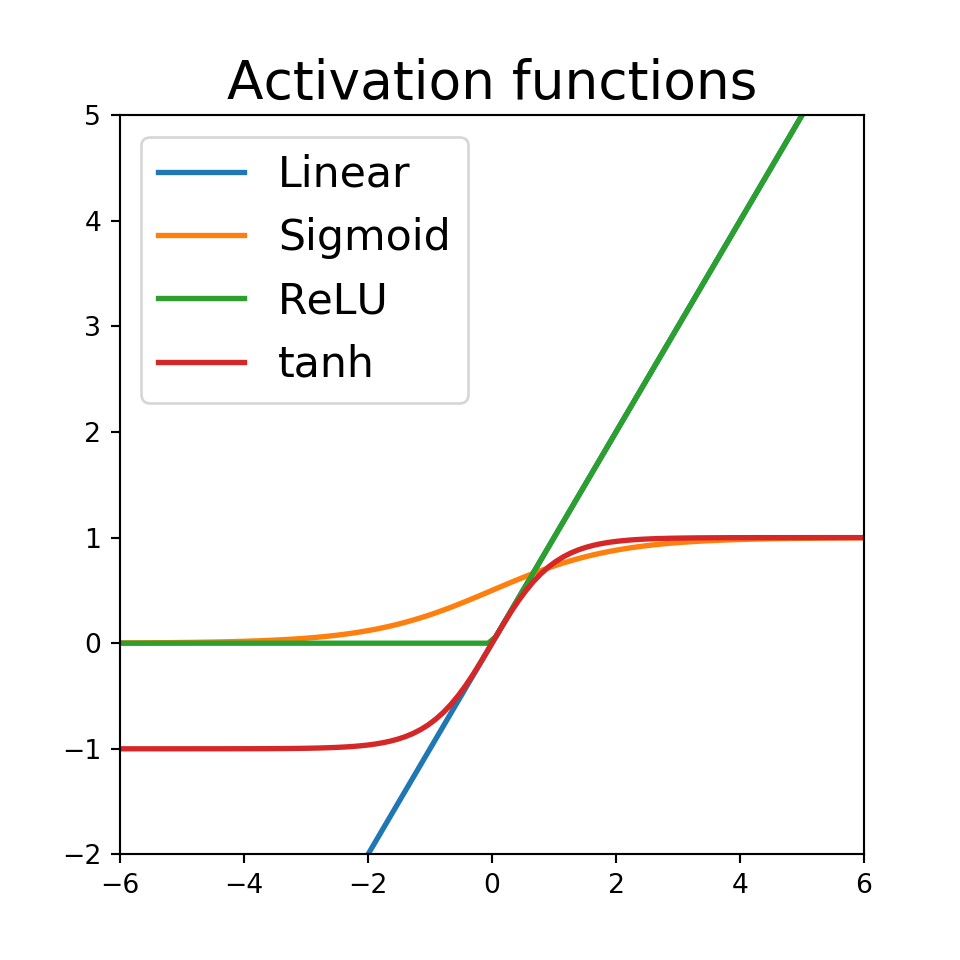
\includegraphics[width=0.7\linewidth]{0101-intro_files/figure-latex/unnamed-chunk-10-1} \end{center}

\hypertarget{generate-a-random-array}{%
\subsubsection*{Generate a random array}\label{generate-a-random-array}}
\addcontentsline{toc}{subsubsection}{Generate a random array}

\begin{Shaded}
\begin{Highlighting}[]
\CommentTok{# set the seed}
\NormalTok{np}\OperatorTok{$}\NormalTok{random}\OperatorTok{$}\KeywordTok{seed}\NormalTok{(123L)}
\CommentTok{# generate a random array}
\NormalTok{x =}\StringTok{ }\NormalTok{np}\OperatorTok{$}\NormalTok{random}\OperatorTok{$}\KeywordTok{rand}\NormalTok{(100L)}
\CommentTok{# calculate the y array}
\NormalTok{y =}\StringTok{ }\NormalTok{np}\OperatorTok{$}\KeywordTok{sin}\NormalTok{(x) }\OperatorTok{*}\StringTok{ }\NormalTok{np}\OperatorTok{$}\KeywordTok{power}\NormalTok{(x, 3L) }\OperatorTok{+}\StringTok{ }\NormalTok{3L }\OperatorTok{*}\StringTok{ }\NormalTok{x }\OperatorTok{+}\StringTok{ }\NormalTok{np}\OperatorTok{$}\NormalTok{random}\OperatorTok{$}\KeywordTok{rand}\NormalTok{(100L) }\OperatorTok{*}\StringTok{ }\FloatTok{0.8}

\KeywordTok{plot}\NormalTok{(x, y)}
\end{Highlighting}
\end{Shaded}

\begin{center}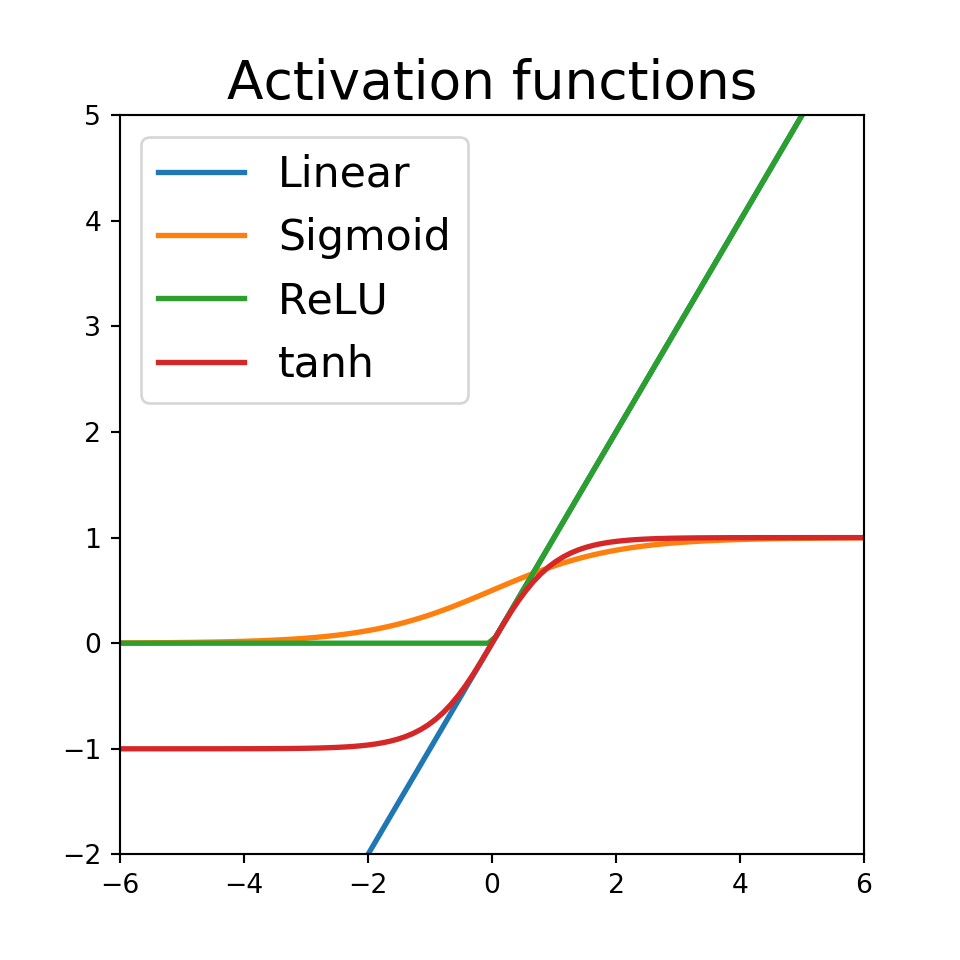
\includegraphics[width=0.7\linewidth]{0101-intro_files/figure-latex/unnamed-chunk-11-1} \end{center}

\hypertarget{convert-a-numpy-array-to-a-pytorch-tensor}{%
\subsubsection*{\texorpdfstring{Convert a \texttt{numpy} array to a PyTorch tensor}{Convert a numpy array to a PyTorch tensor}}\label{convert-a-numpy-array-to-a-pytorch-tensor}}
\addcontentsline{toc}{subsubsection}{Convert a \texttt{numpy} array to a PyTorch tensor}

This is a very common operation that I have seen in examples using PyTorch. Creating the array in \texttt{numpy}. and then convert it to a tensor.

\begin{Shaded}
\begin{Highlighting}[]
\CommentTok{# input array}
\NormalTok{x =}\StringTok{ }\NormalTok{np}\OperatorTok{$}\KeywordTok{array}\NormalTok{(}\KeywordTok{rbind}\NormalTok{(}
            \KeywordTok{c}\NormalTok{(}\DecValTok{0}\NormalTok{,}\DecValTok{0}\NormalTok{,}\DecValTok{1}\NormalTok{),}
            \KeywordTok{c}\NormalTok{(}\DecValTok{0}\NormalTok{,}\DecValTok{1}\NormalTok{,}\DecValTok{1}\NormalTok{),}
            \KeywordTok{c}\NormalTok{(}\DecValTok{1}\NormalTok{,}\DecValTok{0}\NormalTok{,}\DecValTok{1}\NormalTok{),}
            \KeywordTok{c}\NormalTok{(}\DecValTok{1}\NormalTok{,}\DecValTok{1}\NormalTok{,}\DecValTok{1}\NormalTok{)))}

\CommentTok{# the numpy array}
\NormalTok{x}
\CommentTok{#>      [,1] [,2] [,3]}
\CommentTok{#> [1,]    0    0    1}
\CommentTok{#> [2,]    0    1    1}
\CommentTok{#> [3,]    1    0    1}
\CommentTok{#> [4,]    1    1    1}
\end{Highlighting}
\end{Shaded}

\begin{Shaded}
\begin{Highlighting}[]
\CommentTok{# convert the numpy array to float}
\NormalTok{X <-}\StringTok{ }\NormalTok{np}\OperatorTok{$}\KeywordTok{float32}\NormalTok{(x)}
\CommentTok{# convert the numpy array to a float tensor}
\NormalTok{X <-}\StringTok{ }\NormalTok{torch}\OperatorTok{$}\KeywordTok{FloatTensor}\NormalTok{(X)}
\NormalTok{X}
\CommentTok{#> tensor([[0., 0., 1.],}
\CommentTok{#>         [0., 1., 1.],}
\CommentTok{#>         [1., 0., 1.],}
\CommentTok{#>         [1., 1., 1.]])}
\end{Highlighting}
\end{Shaded}

\hypertarget{python-built-in-functions}{%
\subsection{Python built-in functions}\label{python-built-in-functions}}

To access the Python built-in functions we make use of the package \texttt{reticulate} and the function \texttt{import\_builtins()}.

\begin{Shaded}
\begin{Highlighting}[]
\NormalTok{py_bi <-}\StringTok{ }\KeywordTok{import_builtins}\NormalTok{()}
\end{Highlighting}
\end{Shaded}

\hypertarget{length-of-a-dataset}{%
\subsubsection*{Length of a dataset}\label{length-of-a-dataset}}
\addcontentsline{toc}{subsubsection}{Length of a dataset}

\begin{Shaded}
\begin{Highlighting}[]
\NormalTok{py_bi}\OperatorTok{$}\KeywordTok{len}\NormalTok{(train_dataset)}
\CommentTok{#> [1] 60000}
\NormalTok{py_bi}\OperatorTok{$}\KeywordTok{len}\NormalTok{(test_dataset)}
\CommentTok{#> [1] 10000}
\end{Highlighting}
\end{Shaded}

\hypertarget{iterators}{%
\subsubsection*{Iterators}\label{iterators}}
\addcontentsline{toc}{subsubsection}{Iterators}

\begin{Shaded}
\begin{Highlighting}[]
\CommentTok{# iterate through training dataset}
\NormalTok{enum_train_dataset <-}\StringTok{ }\NormalTok{py_bi}\OperatorTok{$}\KeywordTok{enumerate}\NormalTok{(train_dataset)}

\KeywordTok{cat}\NormalTok{(}\KeywordTok{sprintf}\NormalTok{(}\StringTok{"%8s %8s }\CharTok{\textbackslash{}n}\StringTok{"}\NormalTok{, }\StringTok{"index"}\NormalTok{, }\StringTok{"label"}\NormalTok{))}
\CommentTok{#>    index    label}
\ControlFlowTok{for}\NormalTok{ (i }\ControlFlowTok{in} \DecValTok{1}\OperatorTok{:}\NormalTok{py_bi}\OperatorTok{$}\KeywordTok{len}\NormalTok{(train_dataset)) \{}
\NormalTok{    obj <-}\StringTok{ }\NormalTok{reticulate}\OperatorTok{::}\KeywordTok{iter_next}\NormalTok{(enum_train_dataset)}
\NormalTok{    idx   <-}\StringTok{ }\NormalTok{obj[[}\DecValTok{1}\NormalTok{]]        }\CommentTok{# index number}
    \KeywordTok{cat}\NormalTok{(}\KeywordTok{sprintf}\NormalTok{(}\StringTok{"%8d %5d }\CharTok{\textbackslash{}n}\StringTok{"}\NormalTok{, idx, obj[[}\DecValTok{2}\NormalTok{]][[}\DecValTok{2}\NormalTok{]]))}
    
    \ControlFlowTok{if}\NormalTok{ (i }\OperatorTok{>=}\StringTok{ }\DecValTok{100}\NormalTok{) }\ControlFlowTok{break}   \CommentTok{# print only 100 labels}
\NormalTok{\}}
\CommentTok{#>        0     5 }
\CommentTok{#>        1     0 }
\CommentTok{#>        2     4 }
\CommentTok{#>        3     1 }
\CommentTok{#>        4     9 }
\CommentTok{#>        5     2 }
\CommentTok{#>        6     1 }
\CommentTok{#>        7     3 }
\CommentTok{#>        8     1 }
\CommentTok{#>        9     4 }
\CommentTok{#>       10     3 }
\CommentTok{#>       11     5 }
\CommentTok{#>       12     3 }
\CommentTok{#>       13     6 }
\CommentTok{#>       14     1 }
\CommentTok{#>       15     7 }
\CommentTok{#>       16     2 }
\CommentTok{#>       17     8 }
\CommentTok{#>       18     6 }
\CommentTok{#>       19     9 }
\CommentTok{#>       20     4 }
\CommentTok{#>       21     0 }
\CommentTok{#>       22     9 }
\CommentTok{#>       23     1 }
\CommentTok{#>       24     1 }
\CommentTok{#>       25     2 }
\CommentTok{#>       26     4 }
\CommentTok{#>       27     3 }
\CommentTok{#>       28     2 }
\CommentTok{#>       29     7 }
\CommentTok{#>       30     3 }
\CommentTok{#>       31     8 }
\CommentTok{#>       32     6 }
\CommentTok{#>       33     9 }
\CommentTok{#>       34     0 }
\CommentTok{#>       35     5 }
\CommentTok{#>       36     6 }
\CommentTok{#>       37     0 }
\CommentTok{#>       38     7 }
\CommentTok{#>       39     6 }
\CommentTok{#>       40     1 }
\CommentTok{#>       41     8 }
\CommentTok{#>       42     7 }
\CommentTok{#>       43     9 }
\CommentTok{#>       44     3 }
\CommentTok{#>       45     9 }
\CommentTok{#>       46     8 }
\CommentTok{#>       47     5 }
\CommentTok{#>       48     9 }
\CommentTok{#>       49     3 }
\CommentTok{#>       50     3 }
\CommentTok{#>       51     0 }
\CommentTok{#>       52     7 }
\CommentTok{#>       53     4 }
\CommentTok{#>       54     9 }
\CommentTok{#>       55     8 }
\CommentTok{#>       56     0 }
\CommentTok{#>       57     9 }
\CommentTok{#>       58     4 }
\CommentTok{#>       59     1 }
\CommentTok{#>       60     4 }
\CommentTok{#>       61     4 }
\CommentTok{#>       62     6 }
\CommentTok{#>       63     0 }
\CommentTok{#>       64     4 }
\CommentTok{#>       65     5 }
\CommentTok{#>       66     6 }
\CommentTok{#>       67     1 }
\CommentTok{#>       68     0 }
\CommentTok{#>       69     0 }
\CommentTok{#>       70     1 }
\CommentTok{#>       71     7 }
\CommentTok{#>       72     1 }
\CommentTok{#>       73     6 }
\CommentTok{#>       74     3 }
\CommentTok{#>       75     0 }
\CommentTok{#>       76     2 }
\CommentTok{#>       77     1 }
\CommentTok{#>       78     1 }
\CommentTok{#>       79     7 }
\CommentTok{#>       80     9 }
\CommentTok{#>       81     0 }
\CommentTok{#>       82     2 }
\CommentTok{#>       83     6 }
\CommentTok{#>       84     7 }
\CommentTok{#>       85     8 }
\CommentTok{#>       86     3 }
\CommentTok{#>       87     9 }
\CommentTok{#>       88     0 }
\CommentTok{#>       89     4 }
\CommentTok{#>       90     6 }
\CommentTok{#>       91     7 }
\CommentTok{#>       92     4 }
\CommentTok{#>       93     6 }
\CommentTok{#>       94     8 }
\CommentTok{#>       95     0 }
\CommentTok{#>       96     7 }
\CommentTok{#>       97     8 }
\CommentTok{#>       98     3 }
\CommentTok{#>       99     1}
\end{Highlighting}
\end{Shaded}

\hypertarget{types-and-instances}{%
\subsubsection*{Types and instances}\label{types-and-instances}}
\addcontentsline{toc}{subsubsection}{Types and instances}

\begin{Shaded}
\begin{Highlighting}[]
\CommentTok{# get the class of the object}
\NormalTok{py_bi}\OperatorTok{$}\KeywordTok{type}\NormalTok{(train_dataset)}
\CommentTok{#> <class 'torchvision.datasets.mnist.MNIST'>}

\CommentTok{# is train_dataset a torchvision dataset class}
\NormalTok{py_bi}\OperatorTok{$}\KeywordTok{isinstance}\NormalTok{(train_dataset, torchvision}\OperatorTok{$}\NormalTok{datasets}\OperatorTok{$}\NormalTok{mnist}\OperatorTok{$}\NormalTok{MNIST)}
\CommentTok{#> [1] TRUE}
\end{Highlighting}
\end{Shaded}

\hypertarget{rtorch-vs-pytorch-whats-different}{%
\chapter{rTorch vs PyTorch: What's different}\label{rtorch-vs-pytorch-whats-different}}

This chapter will explain the main differences between \texttt{PyTorch} and \texttt{rTorch}.
Most of the things work directly in \texttt{PyTorch} but we need to be aware of some minor differences when working with rTorch.

Here is a review of existing methods.

\begin{Shaded}
\begin{Highlighting}[]
\KeywordTok{library}\NormalTok{(rTorch)}
\end{Highlighting}
\end{Shaded}

\hypertarget{calling-objects-from-pytorch}{%
\section{Calling objects from PyTorch}\label{calling-objects-from-pytorch}}

We use the dollar sign or \texttt{\$} to call a class, function or method from the rTorch modules. In this case, from \texttt{torch} module:

\begin{Shaded}
\begin{Highlighting}[]
\NormalTok{torch}\OperatorTok{$}\NormalTok{tensor}
\CommentTok{#> <built-in method tensor of type>}
\end{Highlighting}
\end{Shaded}

\hypertarget{call-a-module-from-pytorch}{%
\section{Call a module from PyTorch}\label{call-a-module-from-pytorch}}

\begin{Shaded}
\begin{Highlighting}[]
\CommentTok{# these are the equivalents of import module}
\NormalTok{nn          <-}\StringTok{ }\NormalTok{torch}\OperatorTok{$}\NormalTok{nn}
\NormalTok{transforms  <-}\StringTok{ }\NormalTok{torchvision}\OperatorTok{$}\NormalTok{transforms}
\NormalTok{dsets       <-}\StringTok{ }\NormalTok{torchvision}\OperatorTok{$}\NormalTok{datasets}
\end{Highlighting}
\end{Shaded}

Then we can proceed to extract classes, methods and functions from the \texttt{nn}, \texttt{transforms}, and \texttt{dsets} objects.

\hypertarget{show-the-attributes-methods-of-a-class-or-pytorch-object}{%
\section{Show the attributes (methods) of a class or PyTorch object}\label{show-the-attributes-methods-of-a-class-or-pytorch-object}}

Sometimes we are interested in knowing the internal components of a class. In that case, we use the reticulate function \texttt{py\_list\_attributes()}.

\begin{Shaded}
\begin{Highlighting}[]
\NormalTok{local_folder <-}\StringTok{ '../datasets/mnist_digits'}
\NormalTok{train_dataset =}\StringTok{ }\NormalTok{torchvision}\OperatorTok{$}\NormalTok{datasets}\OperatorTok{$}\KeywordTok{MNIST}\NormalTok{(}\DataTypeTok{root =}\NormalTok{ local_folder, }
                                           \DataTypeTok{train =} \OtherTok{TRUE}\NormalTok{, }
                                           \DataTypeTok{transform =}\NormalTok{ transforms}\OperatorTok{$}\KeywordTok{ToTensor}\NormalTok{(),}
                                           \DataTypeTok{download =} \OtherTok{TRUE}\NormalTok{)}

\NormalTok{train_dataset}
\CommentTok{#> Dataset MNIST}
\CommentTok{#>     Number of datapoints: 60000}
\CommentTok{#>     Root location: ../datasets/mnist_digits}
\CommentTok{#>     Split: Train}
\end{Highlighting}
\end{Shaded}

\begin{Shaded}
\begin{Highlighting}[]
\NormalTok{reticulate}\OperatorTok{::}\KeywordTok{py_list_attributes}\NormalTok{(train_dataset)}
\CommentTok{#>  [1] "__add__"                "__class__"             }
\CommentTok{#>  [3] "__delattr__"            "__dict__"              }
\CommentTok{#>  [5] "__dir__"                "__doc__"               }
\CommentTok{#>  [7] "__eq__"                 "__format__"            }
\CommentTok{#>  [9] "__ge__"                 "__getattribute__"      }
\CommentTok{#> [11] "__getitem__"            "__gt__"                }
\CommentTok{#> [13] "__hash__"               "__init__"              }
\CommentTok{#> [15] "__init_subclass__"      "__le__"                }
\CommentTok{#> [17] "__len__"                "__lt__"                }
\CommentTok{#> [19] "__module__"             "__ne__"                }
\CommentTok{#> [21] "__new__"                "__reduce__"            }
\CommentTok{#> [23] "__reduce_ex__"          "__repr__"              }
\CommentTok{#> [25] "__setattr__"            "__sizeof__"            }
\CommentTok{#> [27] "__str__"                "__subclasshook__"      }
\CommentTok{#> [29] "__weakref__"            "_check_exists"         }
\CommentTok{#> [31] "_format_transform_repr" "_repr_indent"          }
\CommentTok{#> [33] "class_to_idx"           "classes"               }
\CommentTok{#> [35] "data"                   "download"              }
\CommentTok{#> [37] "extra_repr"             "extract_gzip"          }
\CommentTok{#> [39] "processed_folder"       "raw_folder"            }
\CommentTok{#> [41] "root"                   "target_transform"      }
\CommentTok{#> [43] "targets"                "test_data"             }
\CommentTok{#> [45] "test_file"              "test_labels"           }
\CommentTok{#> [47] "train"                  "train_data"            }
\CommentTok{#> [49] "train_labels"           "training_file"         }
\CommentTok{#> [51] "transform"              "transforms"            }
\CommentTok{#> [53] "urls"}
\end{Highlighting}
\end{Shaded}

Knowing the internal methods of a class could be useful when we want to refer to a specific property of such class. For example, from the list above, we know that the object \texttt{train\_dataset} has an attribute \texttt{\_\_len\_\_}. We can call it like this:

\begin{Shaded}
\begin{Highlighting}[]
\NormalTok{train_dataset}\OperatorTok{$}\StringTok{`}\DataTypeTok{__len__}\StringTok{`}\NormalTok{()}
\CommentTok{#> [1] 60000}
\end{Highlighting}
\end{Shaded}

\hypertarget{enumeration}{%
\section{Enumeration}\label{enumeration}}

\begin{Shaded}
\begin{Highlighting}[]

\NormalTok{x_train =}\StringTok{ }\KeywordTok{array}\NormalTok{(}\KeywordTok{c}\NormalTok{(}\FloatTok{3.3}\NormalTok{, }\FloatTok{4.4}\NormalTok{, }\FloatTok{5.5}\NormalTok{, }\FloatTok{6.71}\NormalTok{, }\FloatTok{6.93}\NormalTok{, }\FloatTok{4.168}\NormalTok{, }
                  \FloatTok{9.779}\NormalTok{, }\FloatTok{6.182}\NormalTok{, }\FloatTok{7.59}\NormalTok{, }\FloatTok{2.167}\NormalTok{, }\FloatTok{7.042}\NormalTok{,}
                  \FloatTok{10.791}\NormalTok{, }\FloatTok{5.313}\NormalTok{, }\FloatTok{7.997}\NormalTok{, }\FloatTok{3.1}\NormalTok{), }\DataTypeTok{dim =} \KeywordTok{c}\NormalTok{(}\DecValTok{15}\NormalTok{,}\DecValTok{1}\NormalTok{))}

\NormalTok{x_train <-}\StringTok{ }\KeywordTok{r_to_py}\NormalTok{(x_train)}
\NormalTok{x_train <-}\StringTok{ }\NormalTok{torch}\OperatorTok{$}\KeywordTok{from_numpy}\NormalTok{(x_train)         }\CommentTok{# convert to tensor}
\NormalTok{x_train <-}\StringTok{ }\NormalTok{x_train}\OperatorTok{$}\KeywordTok{type}\NormalTok{(torch}\OperatorTok{$}\NormalTok{FloatTensor)   }\CommentTok{# make it a a FloatTensor}

\NormalTok{x_train}
\CommentTok{#> tensor([[ 3.3000],}
\CommentTok{#>         [ 4.4000],}
\CommentTok{#>         [ 5.5000],}
\CommentTok{#>         [ 6.7100],}
\CommentTok{#>         [ 6.9300],}
\CommentTok{#>         [ 4.1680],}
\CommentTok{#>         [ 9.7790],}
\CommentTok{#>         [ 6.1820],}
\CommentTok{#>         [ 7.5900],}
\CommentTok{#>         [ 2.1670],}
\CommentTok{#>         [ 7.0420],}
\CommentTok{#>         [10.7910],}
\CommentTok{#>         [ 5.3130],}
\CommentTok{#>         [ 7.9970],}
\CommentTok{#>         [ 3.1000]])}
\end{Highlighting}
\end{Shaded}

\begin{Shaded}
\begin{Highlighting}[]
\NormalTok{x_train}\OperatorTok{$}\KeywordTok{nelement}\NormalTok{()    }\CommentTok{# number of elements in the tensor}
\CommentTok{#> [1] 15}
\end{Highlighting}
\end{Shaded}

\hypertarget{how-to-iterate}{%
\section{How to iterate}\label{how-to-iterate}}

\hypertarget{using-enumerate-and-iterate}{%
\subsection{\texorpdfstring{Using \texttt{enumerate} and \texttt{iterate}}{Using enumerate and iterate}}\label{using-enumerate-and-iterate}}

\begin{Shaded}
\begin{Highlighting}[]
\NormalTok{py =}\StringTok{ }\KeywordTok{import_builtins}\NormalTok{()}

\NormalTok{enum_x_train =}\StringTok{ }\NormalTok{py}\OperatorTok{$}\KeywordTok{enumerate}\NormalTok{(x_train)}
\NormalTok{enum_x_train}
\CommentTok{#> <enumerate>}

\NormalTok{py}\OperatorTok{$}\KeywordTok{len}\NormalTok{(x_train)}
\CommentTok{#> [1] 15}
\end{Highlighting}
\end{Shaded}

\begin{Shaded}
\begin{Highlighting}[]
\NormalTok{xit =}\StringTok{ }\KeywordTok{iterate}\NormalTok{(enum_x_train, }\DataTypeTok{simplify =} \OtherTok{TRUE}\NormalTok{)}
\NormalTok{xit}
\CommentTok{#> [[1]]}
\CommentTok{#> [[1]][[1]]}
\CommentTok{#> [1] 0}
\CommentTok{#> }
\CommentTok{#> [[1]][[2]]}
\CommentTok{#> tensor([3.3000])}
\CommentTok{#> }
\CommentTok{#> }
\CommentTok{#> [[2]]}
\CommentTok{#> [[2]][[1]]}
\CommentTok{#> [1] 1}
\CommentTok{#> }
\CommentTok{#> [[2]][[2]]}
\CommentTok{#> tensor([4.4000])}
\CommentTok{#> }
\CommentTok{#> }
\CommentTok{#> [[3]]}
\CommentTok{#> [[3]][[1]]}
\CommentTok{#> [1] 2}
\CommentTok{#> }
\CommentTok{#> [[3]][[2]]}
\CommentTok{#> tensor([5.5000])}
\CommentTok{#> }
\CommentTok{#> }
\CommentTok{#> [[4]]}
\CommentTok{#> [[4]][[1]]}
\CommentTok{#> [1] 3}
\CommentTok{#> }
\CommentTok{#> [[4]][[2]]}
\CommentTok{#> tensor([6.7100])}
\CommentTok{#> }
\CommentTok{#> }
\CommentTok{#> [[5]]}
\CommentTok{#> [[5]][[1]]}
\CommentTok{#> [1] 4}
\CommentTok{#> }
\CommentTok{#> [[5]][[2]]}
\CommentTok{#> tensor([6.9300])}
\CommentTok{#> }
\CommentTok{#> }
\CommentTok{#> [[6]]}
\CommentTok{#> [[6]][[1]]}
\CommentTok{#> [1] 5}
\CommentTok{#> }
\CommentTok{#> [[6]][[2]]}
\CommentTok{#> tensor([4.1680])}
\CommentTok{#> }
\CommentTok{#> }
\CommentTok{#> [[7]]}
\CommentTok{#> [[7]][[1]]}
\CommentTok{#> [1] 6}
\CommentTok{#> }
\CommentTok{#> [[7]][[2]]}
\CommentTok{#> tensor([9.7790])}
\CommentTok{#> }
\CommentTok{#> }
\CommentTok{#> [[8]]}
\CommentTok{#> [[8]][[1]]}
\CommentTok{#> [1] 7}
\CommentTok{#> }
\CommentTok{#> [[8]][[2]]}
\CommentTok{#> tensor([6.1820])}
\CommentTok{#> }
\CommentTok{#> }
\CommentTok{#> [[9]]}
\CommentTok{#> [[9]][[1]]}
\CommentTok{#> [1] 8}
\CommentTok{#> }
\CommentTok{#> [[9]][[2]]}
\CommentTok{#> tensor([7.5900])}
\CommentTok{#> }
\CommentTok{#> }
\CommentTok{#> [[10]]}
\CommentTok{#> [[10]][[1]]}
\CommentTok{#> [1] 9}
\CommentTok{#> }
\CommentTok{#> [[10]][[2]]}
\CommentTok{#> tensor([2.1670])}
\CommentTok{#> }
\CommentTok{#> }
\CommentTok{#> [[11]]}
\CommentTok{#> [[11]][[1]]}
\CommentTok{#> [1] 10}
\CommentTok{#> }
\CommentTok{#> [[11]][[2]]}
\CommentTok{#> tensor([7.0420])}
\CommentTok{#> }
\CommentTok{#> }
\CommentTok{#> [[12]]}
\CommentTok{#> [[12]][[1]]}
\CommentTok{#> [1] 11}
\CommentTok{#> }
\CommentTok{#> [[12]][[2]]}
\CommentTok{#> tensor([10.7910])}
\CommentTok{#> }
\CommentTok{#> }
\CommentTok{#> [[13]]}
\CommentTok{#> [[13]][[1]]}
\CommentTok{#> [1] 12}
\CommentTok{#> }
\CommentTok{#> [[13]][[2]]}
\CommentTok{#> tensor([5.3130])}
\CommentTok{#> }
\CommentTok{#> }
\CommentTok{#> [[14]]}
\CommentTok{#> [[14]][[1]]}
\CommentTok{#> [1] 13}
\CommentTok{#> }
\CommentTok{#> [[14]][[2]]}
\CommentTok{#> tensor([7.9970])}
\CommentTok{#> }
\CommentTok{#> }
\CommentTok{#> [[15]]}
\CommentTok{#> [[15]][[1]]}
\CommentTok{#> [1] 14}
\CommentTok{#> }
\CommentTok{#> [[15]][[2]]}
\CommentTok{#> tensor([3.1000])}
\end{Highlighting}
\end{Shaded}

\hypertarget{using-a-for-loop-to-iterate}{%
\subsection{\texorpdfstring{Using a \texttt{for-loop} to iterate}{Using a for-loop to iterate}}\label{using-a-for-loop-to-iterate}}

\begin{Shaded}
\begin{Highlighting}[]
\CommentTok{# reset the iterator}
\NormalTok{enum_x_train =}\StringTok{ }\NormalTok{py}\OperatorTok{$}\KeywordTok{enumerate}\NormalTok{(x_train)}

\ControlFlowTok{for}\NormalTok{ (i }\ControlFlowTok{in} \DecValTok{1}\OperatorTok{:}\NormalTok{py}\OperatorTok{$}\KeywordTok{len}\NormalTok{(x_train)) \{}
\NormalTok{    obj <-}\StringTok{ }\KeywordTok{iter_next}\NormalTok{(enum_x_train)    }\CommentTok{# next item}
    \KeywordTok{cat}\NormalTok{(obj[[}\DecValTok{1}\NormalTok{]], }\StringTok{"}\CharTok{\textbackslash{}t}\StringTok{"}\NormalTok{)     }\CommentTok{# 1st part or index}
    \KeywordTok{print}\NormalTok{(obj[[}\DecValTok{2}\NormalTok{]])         }\CommentTok{# 2nd part or tensor}
\NormalTok{\}}
\CommentTok{#> 0    tensor([3.3000])}
\CommentTok{#> 1    tensor([4.4000])}
\CommentTok{#> 2    tensor([5.5000])}
\CommentTok{#> 3    tensor([6.7100])}
\CommentTok{#> 4    tensor([6.9300])}
\CommentTok{#> 5    tensor([4.1680])}
\CommentTok{#> 6    tensor([9.7790])}
\CommentTok{#> 7    tensor([6.1820])}
\CommentTok{#> 8    tensor([7.5900])}
\CommentTok{#> 9    tensor([2.1670])}
\CommentTok{#> 10   tensor([7.0420])}
\CommentTok{#> 11   tensor([10.7910])}
\CommentTok{#> 12   tensor([5.3130])}
\CommentTok{#> 13   tensor([7.9970])}
\CommentTok{#> 14   tensor([3.1000])}
\end{Highlighting}
\end{Shaded}

\begin{quote}
We will find very frequently this kind of iterators when we read a dataset using \texttt{torchvision}. There are different ways to iterate through these objects.
\end{quote}

\hypertarget{zero-gradient}{%
\section{Zero gradient}\label{zero-gradient}}

The zero gradient was one of the most difficult to implement in R if we don't pay attention to the content of the objects carrying the weights and biases. This happens when the algorithm written in PyTorch is not immediately translatable to rTorch. This can be appreciated in this example.

\hypertarget{version-in-python}{%
\subsection{Version in Python}\label{version-in-python}}

\begin{Shaded}
\begin{Highlighting}[]
\ImportTok{import}\NormalTok{ numpy }\ImportTok{as}\NormalTok{ np}
\ImportTok{import}\NormalTok{ torch}

\NormalTok{torch.manual_seed(}\DecValTok{0}\NormalTok{)  }\CommentTok{# reproducible}

\CommentTok{# Input (temp, rainfall, humidity)}
\CommentTok{#> <torch._C.Generator object at 0x7f631a5cae10>}
\NormalTok{inputs }\OperatorTok{=}\NormalTok{ np.array([[}\DecValTok{73}\NormalTok{, }\DecValTok{67}\NormalTok{, }\DecValTok{43}\NormalTok{],}
\NormalTok{                   [}\DecValTok{91}\NormalTok{, }\DecValTok{88}\NormalTok{, }\DecValTok{64}\NormalTok{],}
\NormalTok{                   [}\DecValTok{87}\NormalTok{, }\DecValTok{134}\NormalTok{, }\DecValTok{58}\NormalTok{],}
\NormalTok{                   [}\DecValTok{102}\NormalTok{, }\DecValTok{43}\NormalTok{, }\DecValTok{37}\NormalTok{],}
\NormalTok{                   [}\DecValTok{69}\NormalTok{, }\DecValTok{96}\NormalTok{, }\DecValTok{70}\NormalTok{]], dtype}\OperatorTok{=}\StringTok{'float32'}\NormalTok{)}

\CommentTok{# Targets (apples, oranges)}
\NormalTok{targets }\OperatorTok{=}\NormalTok{ np.array([[}\DecValTok{56}\NormalTok{, }\DecValTok{70}\NormalTok{],}
\NormalTok{                    [}\DecValTok{81}\NormalTok{, }\DecValTok{101}\NormalTok{],}
\NormalTok{                    [}\DecValTok{119}\NormalTok{, }\DecValTok{133}\NormalTok{],}
\NormalTok{                    [}\DecValTok{22}\NormalTok{, }\DecValTok{37}\NormalTok{],}
\NormalTok{                    [}\DecValTok{103}\NormalTok{, }\DecValTok{119}\NormalTok{]], dtype}\OperatorTok{=}\StringTok{'float32'}\NormalTok{)}
                    

\CommentTok{# Convert inputs and targets to tensors}
\NormalTok{inputs }\OperatorTok{=}\NormalTok{ torch.from_numpy(inputs)}
\NormalTok{targets }\OperatorTok{=}\NormalTok{ torch.from_numpy(targets)}

\CommentTok{# random weights and biases}
\NormalTok{w }\OperatorTok{=}\NormalTok{ torch.randn(}\DecValTok{2}\NormalTok{, }\DecValTok{3}\NormalTok{, requires_grad}\OperatorTok{=}\VariableTok{True}\NormalTok{)}
\NormalTok{b }\OperatorTok{=}\NormalTok{ torch.randn(}\DecValTok{2}\NormalTok{, requires_grad}\OperatorTok{=}\VariableTok{True}\NormalTok{)}

\CommentTok{# function for the model}
\KeywordTok{def}\NormalTok{ model(x):}
\NormalTok{  wt }\OperatorTok{=}\NormalTok{ w.t()}
\NormalTok{  mm }\OperatorTok{=}\NormalTok{ x }\OperatorTok{@}\NormalTok{ w.t()}
  \ControlFlowTok{return}\NormalTok{ x }\OperatorTok{@}\NormalTok{ w.t() }\OperatorTok{+}\NormalTok{ b       }\CommentTok{# @ represents matrix multiplication in PyTorch}

\CommentTok{# MSE loss function}
\KeywordTok{def}\NormalTok{ mse(t1, t2):}
\NormalTok{  diff }\OperatorTok{=}\NormalTok{ t1 }\OperatorTok{-}\NormalTok{ t2}
  \ControlFlowTok{return}\NormalTok{ torch.}\BuiltInTok{sum}\NormalTok{(diff }\OperatorTok{*}\NormalTok{ diff) }\OperatorTok{/}\NormalTok{ diff.numel()}

\CommentTok{# Running all together}
\CommentTok{# Train for 100 epochs}
\ControlFlowTok{for}\NormalTok{ i }\KeywordTok{in} \BuiltInTok{range}\NormalTok{(}\DecValTok{100}\NormalTok{):}
\NormalTok{  preds }\OperatorTok{=}\NormalTok{ model(inputs)}
\NormalTok{  loss }\OperatorTok{=}\NormalTok{ mse(preds, targets)}
\NormalTok{  loss.backward()}
  \ControlFlowTok{with}\NormalTok{ torch.no_grad():}
\NormalTok{    w }\OperatorTok{-=}\NormalTok{ w.grad }\OperatorTok{*} \FloatTok{0.00001}
\NormalTok{    b }\OperatorTok{-=}\NormalTok{ b.grad }\OperatorTok{*} \FloatTok{0.00001}
\NormalTok{    w_gz }\OperatorTok{=}\NormalTok{ w.grad.zero_()}
\NormalTok{    b_gz }\OperatorTok{=}\NormalTok{ b.grad.zero_()}
    
\CommentTok{# Calculate loss}
\NormalTok{preds }\OperatorTok{=}\NormalTok{ model(inputs)}
\NormalTok{loss }\OperatorTok{=}\NormalTok{ mse(preds, targets)}
\BuiltInTok{print}\NormalTok{(}\StringTok{"Loss: "}\NormalTok{, loss)    }

\CommentTok{# predictions}
\CommentTok{#> Loss:  tensor(1270.1234, grad_fn=<DivBackward0>)}
\BuiltInTok{print}\NormalTok{(}\StringTok{"}\CharTok{\textbackslash{}n}\StringTok{Predictions:"}\NormalTok{)}
\CommentTok{#> }
\CommentTok{#> Predictions:}
\NormalTok{preds}

\CommentTok{# Targets}
\CommentTok{#> tensor([[ 69.3122,  80.2639],}
\CommentTok{#>         [ 73.7528,  97.2381],}
\CommentTok{#>         [118.3933, 124.7628],}
\CommentTok{#>         [ 89.6111,  93.0286],}
\CommentTok{#>         [ 47.3014,  80.6467]], grad_fn=<AddBackward0>)}
\BuiltInTok{print}\NormalTok{(}\StringTok{"}\CharTok{\textbackslash{}n}\StringTok{Targets:"}\NormalTok{)}
\CommentTok{#> }
\CommentTok{#> Targets:}
\NormalTok{targets}
\CommentTok{#> tensor([[ 56.,  70.],}
\CommentTok{#>         [ 81., 101.],}
\CommentTok{#>         [119., 133.],}
\CommentTok{#>         [ 22.,  37.],}
\CommentTok{#>         [103., 119.]])}
\end{Highlighting}
\end{Shaded}

\hypertarget{version-in-r}{%
\subsection{Version in R}\label{version-in-r}}

\begin{Shaded}
\begin{Highlighting}[]
\KeywordTok{library}\NormalTok{(rTorch)}

\NormalTok{torch}\OperatorTok{$}\KeywordTok{manual_seed}\NormalTok{(}\DecValTok{0}\NormalTok{)}
\CommentTok{#> <torch._C.Generator>}

\NormalTok{device =}\StringTok{ }\NormalTok{torch}\OperatorTok{$}\KeywordTok{device}\NormalTok{(}\StringTok{'cpu'}\NormalTok{)}
\CommentTok{# Input (temp, rainfall, humidity)}
\NormalTok{inputs =}\StringTok{ }\NormalTok{np}\OperatorTok{$}\KeywordTok{array}\NormalTok{(}\KeywordTok{list}\NormalTok{(}\KeywordTok{list}\NormalTok{(}\DecValTok{73}\NormalTok{, }\DecValTok{67}\NormalTok{, }\DecValTok{43}\NormalTok{),}
                   \KeywordTok{list}\NormalTok{(}\DecValTok{91}\NormalTok{, }\DecValTok{88}\NormalTok{, }\DecValTok{64}\NormalTok{),}
                   \KeywordTok{list}\NormalTok{(}\DecValTok{87}\NormalTok{, }\DecValTok{134}\NormalTok{, }\DecValTok{58}\NormalTok{),}
                   \KeywordTok{list}\NormalTok{(}\DecValTok{102}\NormalTok{, }\DecValTok{43}\NormalTok{, }\DecValTok{37}\NormalTok{),}
                   \KeywordTok{list}\NormalTok{(}\DecValTok{69}\NormalTok{, }\DecValTok{96}\NormalTok{, }\DecValTok{70}\NormalTok{)), }\DataTypeTok{dtype=}\StringTok{'float32'}\NormalTok{)}

\CommentTok{# Targets (apples, oranges)}
\NormalTok{targets =}\StringTok{ }\NormalTok{np}\OperatorTok{$}\KeywordTok{array}\NormalTok{(}\KeywordTok{list}\NormalTok{(}\KeywordTok{list}\NormalTok{(}\DecValTok{56}\NormalTok{, }\DecValTok{70}\NormalTok{), }
                    \KeywordTok{list}\NormalTok{(}\DecValTok{81}\NormalTok{, }\DecValTok{101}\NormalTok{),}
                    \KeywordTok{list}\NormalTok{(}\DecValTok{119}\NormalTok{, }\DecValTok{133}\NormalTok{),}
                    \KeywordTok{list}\NormalTok{(}\DecValTok{22}\NormalTok{, }\DecValTok{37}\NormalTok{), }
                    \KeywordTok{list}\NormalTok{(}\DecValTok{103}\NormalTok{, }\DecValTok{119}\NormalTok{)), }\DataTypeTok{dtype=}\StringTok{'float32'}\NormalTok{)}


\CommentTok{# Convert inputs and targets to tensors}
\NormalTok{inputs =}\StringTok{ }\NormalTok{torch}\OperatorTok{$}\KeywordTok{from_numpy}\NormalTok{(inputs)}
\NormalTok{targets =}\StringTok{ }\NormalTok{torch}\OperatorTok{$}\KeywordTok{from_numpy}\NormalTok{(targets)}

\CommentTok{# random numbers for weights and biases. Then convert to double()}
\NormalTok{torch}\OperatorTok{$}\KeywordTok{set_default_dtype}\NormalTok{(torch}\OperatorTok{$}\NormalTok{float64)}

\NormalTok{w =}\StringTok{ }\NormalTok{torch}\OperatorTok{$}\KeywordTok{randn}\NormalTok{(2L, 3L, }\DataTypeTok{requires_grad=}\OtherTok{TRUE}\NormalTok{) }\CommentTok{#$double()}
\NormalTok{b =}\StringTok{ }\NormalTok{torch}\OperatorTok{$}\KeywordTok{randn}\NormalTok{(2L, }\DataTypeTok{requires_grad=}\OtherTok{TRUE}\NormalTok{) }\CommentTok{#$double()}

\NormalTok{model <-}\StringTok{ }\ControlFlowTok{function}\NormalTok{(x) \{}
\NormalTok{  wt <-}\StringTok{ }\NormalTok{w}\OperatorTok{$}\KeywordTok{t}\NormalTok{()}
  \KeywordTok{return}\NormalTok{(torch}\OperatorTok{$}\KeywordTok{add}\NormalTok{(torch}\OperatorTok{$}\KeywordTok{mm}\NormalTok{(x, wt), b))}
\NormalTok{\}}

\CommentTok{# MSE loss}
\NormalTok{mse =}\StringTok{ }\ControlFlowTok{function}\NormalTok{(t1, t2) \{}
\NormalTok{  diff <-}\StringTok{ }\NormalTok{torch}\OperatorTok{$}\KeywordTok{sub}\NormalTok{(t1, t2)}
\NormalTok{  mul <-}\StringTok{ }\NormalTok{torch}\OperatorTok{$}\KeywordTok{sum}\NormalTok{(torch}\OperatorTok{$}\KeywordTok{mul}\NormalTok{(diff, diff))}
  \KeywordTok{return}\NormalTok{(torch}\OperatorTok{$}\KeywordTok{div}\NormalTok{(mul, diff}\OperatorTok{$}\KeywordTok{numel}\NormalTok{()))}
\NormalTok{\}}

\CommentTok{# Running all together}
\CommentTok{# Adjust weights and reset gradients}
\ControlFlowTok{for}\NormalTok{ (i }\ControlFlowTok{in} \DecValTok{1}\OperatorTok{:}\DecValTok{100}\NormalTok{) \{}
\NormalTok{  preds =}\StringTok{ }\KeywordTok{model}\NormalTok{(inputs)}
\NormalTok{  loss =}\StringTok{ }\KeywordTok{mse}\NormalTok{(preds, targets)}
\NormalTok{  loss}\OperatorTok{$}\KeywordTok{backward}\NormalTok{()}
  \KeywordTok{with}\NormalTok{(torch}\OperatorTok{$}\KeywordTok{no_grad}\NormalTok{(), \{}
\NormalTok{    w}\OperatorTok{$}\NormalTok{data <-}\StringTok{ }\NormalTok{torch}\OperatorTok{$}\KeywordTok{sub}\NormalTok{(w}\OperatorTok{$}\NormalTok{data, torch}\OperatorTok{$}\KeywordTok{mul}\NormalTok{(w}\OperatorTok{$}\NormalTok{grad, torch}\OperatorTok{$}\KeywordTok{scalar_tensor}\NormalTok{(}\FloatTok{1e-5}\NormalTok{)))}
\NormalTok{    b}\OperatorTok{$}\NormalTok{data <-}\StringTok{ }\NormalTok{torch}\OperatorTok{$}\KeywordTok{sub}\NormalTok{(b}\OperatorTok{$}\NormalTok{data, torch}\OperatorTok{$}\KeywordTok{mul}\NormalTok{(b}\OperatorTok{$}\NormalTok{grad, torch}\OperatorTok{$}\KeywordTok{scalar_tensor}\NormalTok{(}\FloatTok{1e-5}\NormalTok{)))}
    
\NormalTok{    w}\OperatorTok{$}\NormalTok{grad}\OperatorTok{$}\KeywordTok{zero_}\NormalTok{()}
\NormalTok{    b}\OperatorTok{$}\NormalTok{grad}\OperatorTok{$}\KeywordTok{zero_}\NormalTok{()}
\NormalTok{  \})}
\NormalTok{\}}

\CommentTok{# Calculate loss}
\NormalTok{preds =}\StringTok{ }\KeywordTok{model}\NormalTok{(inputs)}
\NormalTok{loss =}\StringTok{ }\KeywordTok{mse}\NormalTok{(preds, targets)}
\KeywordTok{cat}\NormalTok{(}\StringTok{"Loss: "}\NormalTok{); }\KeywordTok{print}\NormalTok{(loss)}
\CommentTok{#> Loss:}
\CommentTok{#> tensor(1270.1237, grad_fn=<DivBackward0>)}

\CommentTok{# predictions}
\KeywordTok{cat}\NormalTok{(}\StringTok{"}\CharTok{\textbackslash{}n}\StringTok{Predictions:}\CharTok{\textbackslash{}n}\StringTok{"}\NormalTok{)}
\CommentTok{#> }
\CommentTok{#> Predictions:}
\NormalTok{preds}
\CommentTok{#> tensor([[ 69.3122,  80.2639],}
\CommentTok{#>         [ 73.7528,  97.2381],}
\CommentTok{#>         [118.3933, 124.7628],}
\CommentTok{#>         [ 89.6111,  93.0286],}
\CommentTok{#>         [ 47.3013,  80.6467]], grad_fn=<AddBackward0>)}

\CommentTok{# Targets}
\KeywordTok{cat}\NormalTok{(}\StringTok{"}\CharTok{\textbackslash{}n}\StringTok{Targets:}\CharTok{\textbackslash{}n}\StringTok{"}\NormalTok{)}
\CommentTok{#> }
\CommentTok{#> Targets:}
\NormalTok{targets}
\CommentTok{#> tensor([[ 56.,  70.],}
\CommentTok{#>         [ 81., 101.],}
\CommentTok{#>         [119., 133.],}
\CommentTok{#>         [ 22.,  37.],}
\CommentTok{#>         [103., 119.]])}
\end{Highlighting}
\end{Shaded}

Notice that while in Python, the tensor operation, gradient of the weights times the \textbf{Learning Rate}, is:

\[w = -w + \nabla w \; \alpha\]

is a very straight forwward and clean code:

\begin{Shaded}
\begin{Highlighting}[]
\NormalTok{w }\OperatorTok{-=}\NormalTok{ w.grad }\OperatorTok{*} \FloatTok{1e-5}
\end{Highlighting}
\end{Shaded}

In R shows a little bit more convoluted:

\begin{Shaded}
\begin{Highlighting}[]
\NormalTok{w}\OperatorTok{$}\NormalTok{data <-}\StringTok{ }\NormalTok{torch}\OperatorTok{$}\KeywordTok{sub}\NormalTok{(w}\OperatorTok{$}\NormalTok{data, torch}\OperatorTok{$}\KeywordTok{mul}\NormalTok{(w}\OperatorTok{$}\NormalTok{grad, torch}\OperatorTok{$}\KeywordTok{scalar_tensor}\NormalTok{(}\FloatTok{1e-5}\NormalTok{)))}
\end{Highlighting}
\end{Shaded}

\hypertarget{transform-a-tensor}{%
\section{Transform a tensor}\label{transform-a-tensor}}

Explain how transform a tensor back and forth to \texttt{numpy}.
Why is this important?

\hypertarget{build-a-model-class}{%
\section{Build a model class}\label{build-a-model-class}}

PyTorch classes cannot not directly instantiated from \texttt{R}. We need an intermediate step to create a class. For this, we use \texttt{reticulate} functions that will read the class implementation in \texttt{Python} code.

\hypertarget{example-1}{%
\subsection{Example 1}\label{example-1}}

\hypertarget{example-2}{%
\subsection{Example 2}\label{example-2}}

\hypertarget{convert-a-tensor-to-numpy-object}{%
\section{\texorpdfstring{Convert a tensor to \texttt{numpy} object}{Convert a tensor to numpy object}}\label{convert-a-tensor-to-numpy-object}}

This is a frequent operation. I have found that this is necessary when

\begin{itemize}
\tightlist
\item
  a numpy function is not implemented in PyTorch
\item
  We need to convert a tensor to R
\item
  Perform a Boolean operation that is not directly available in PyTorch.
\end{itemize}

\hypertarget{convert-a-numpy-object-to-an-r-object}{%
\section{\texorpdfstring{Convert a \texttt{numpy} object to an \texttt{R} object}{Convert a numpy object to an R object}}\label{convert-a-numpy-object-to-an-r-object}}

This is mainly required for these reasons:

\begin{enumerate}
\def\labelenumi{\arabic{enumi}.}
\tightlist
\item
  Create a data structure in R
\item
  Plot using r-base or ggplot2
\item
  Perform an analysis on parts of a tensor
\item
  Use R statistical functions that are not available in PyTorch.
\end{enumerate}

\hypertarget{part-basic-tensor-operations}{%
\part{Basic Tensor Operations}\label{part-basic-tensor-operations}}

\hypertarget{tensors}{%
\chapter{Tensors}\label{tensors}}

We describe the most important PyTorch methods in this chapter.

\hypertarget{arithmetic-of-tensors}{%
\section{Arithmetic of tensors}\label{arithmetic-of-tensors}}

\hypertarget{boolean-operations}{%
\section{Boolean operations}\label{boolean-operations}}

\hypertarget{slicing}{%
\section{Slicing}\label{slicing}}

\hypertarget{example-3}{%
\section{Example}\label{example-3}}

The following example was converted from PyTorch to rTorch to show differences and similarities of both approaches. The original source can be found here:

Source: \url{https://github.com/jcjohnson/pytorch-examples\#pytorch-tensors}

\hypertarget{load-the-libraries}{%
\subsection{Load the libraries}\label{load-the-libraries}}

\begin{Shaded}
\begin{Highlighting}[]
\KeywordTok{library}\NormalTok{(rTorch)}

\NormalTok{device =}\StringTok{ }\NormalTok{torch}\OperatorTok{$}\KeywordTok{device}\NormalTok{(}\StringTok{'cpu'}\NormalTok{)}
\CommentTok{# device = torch.device('cuda') # Uncomment this to run on GPU}

\NormalTok{torch}\OperatorTok{$}\KeywordTok{manual_seed}\NormalTok{(}\DecValTok{0}\NormalTok{)}
\CommentTok{#> <torch._C.Generator>}
\end{Highlighting}
\end{Shaded}

\begin{itemize}
\tightlist
\item
  \texttt{N} is batch size;
\item
  \texttt{D\_in} is input dimension;
\item
  \texttt{H} is hidden dimension;
\item
  \texttt{D\_out} is output dimension.
\end{itemize}

\hypertarget{datasets}{%
\subsection{Datasets}\label{datasets}}

We will create a random dataset for a two layer neural network.

\begin{Shaded}
\begin{Highlighting}[]
\NormalTok{N <-}\StringTok{ }\NormalTok{64L; D_in <-}\StringTok{ }\NormalTok{1000L; H <-}\StringTok{ }\NormalTok{100L; D_out <-}\StringTok{ }\NormalTok{10L}

\CommentTok{# Create random Tensors to hold inputs and outputs}
\NormalTok{x <-}\StringTok{ }\NormalTok{torch}\OperatorTok{$}\KeywordTok{randn}\NormalTok{(N, D_in, }\DataTypeTok{device=}\NormalTok{device)}
\NormalTok{y <-}\StringTok{ }\NormalTok{torch}\OperatorTok{$}\KeywordTok{randn}\NormalTok{(N, D_out, }\DataTypeTok{device=}\NormalTok{device)}
\end{Highlighting}
\end{Shaded}

\begin{Shaded}
\begin{Highlighting}[]
\CommentTok{# Randomly initialize weights}
\NormalTok{w1 <-}\StringTok{ }\NormalTok{torch}\OperatorTok{$}\KeywordTok{randn}\NormalTok{(D_in, H, }\DataTypeTok{device=}\NormalTok{device)   }\CommentTok{# layer 1}
\NormalTok{w2 <-}\StringTok{ }\NormalTok{torch}\OperatorTok{$}\KeywordTok{randn}\NormalTok{(H, D_out, }\DataTypeTok{device=}\NormalTok{device)  }\CommentTok{# layer 2}
\end{Highlighting}
\end{Shaded}

\hypertarget{run-the-model}{%
\subsection{Run the model}\label{run-the-model}}

\begin{Shaded}
\begin{Highlighting}[]
\NormalTok{learning_rate =}\StringTok{ }\FloatTok{1e-6}

\CommentTok{# loop}
\ControlFlowTok{for}\NormalTok{ (t }\ControlFlowTok{in} \DecValTok{1}\OperatorTok{:}\DecValTok{50}\NormalTok{) \{}
  \CommentTok{# Forward pass: compute predicted y}
\NormalTok{  h <-}\StringTok{ }\NormalTok{x}\OperatorTok{$}\KeywordTok{mm}\NormalTok{(w1)}
\NormalTok{  h_relu <-}\StringTok{ }\NormalTok{h}\OperatorTok{$}\KeywordTok{clamp}\NormalTok{(}\DataTypeTok{min=}\DecValTok{0}\NormalTok{)}
\NormalTok{  y_pred <-}\StringTok{ }\NormalTok{h_relu}\OperatorTok{$}\KeywordTok{mm}\NormalTok{(w2)}

  \CommentTok{# Compute and print loss; loss is a scalar, and is stored in a PyTorch Tensor}
  \CommentTok{# of shape (); we can get its value as a Python number with loss.item().}
\NormalTok{  loss <-}\StringTok{ }\NormalTok{(torch}\OperatorTok{$}\KeywordTok{sub}\NormalTok{(y_pred, y))}\OperatorTok{$}\KeywordTok{pow}\NormalTok{(}\DecValTok{2}\NormalTok{)}\OperatorTok{$}\KeywordTok{sum}\NormalTok{()}
  \KeywordTok{cat}\NormalTok{(t, }\StringTok{"}\CharTok{\textbackslash{}t}\StringTok{"}\NormalTok{)}
  \KeywordTok{cat}\NormalTok{(loss}\OperatorTok{$}\KeywordTok{item}\NormalTok{(), }\StringTok{"}\CharTok{\textbackslash{}n}\StringTok{"}\NormalTok{)}

  \CommentTok{# Backprop to compute gradients of w1 and w2 with respect to loss}
\NormalTok{  grad_y_pred <-}\StringTok{ }\NormalTok{torch}\OperatorTok{$}\KeywordTok{mul}\NormalTok{(torch}\OperatorTok{$}\KeywordTok{scalar_tensor}\NormalTok{(}\FloatTok{2.0}\NormalTok{), torch}\OperatorTok{$}\KeywordTok{sub}\NormalTok{(y_pred, y))}
\NormalTok{  grad_w2 <-}\StringTok{ }\NormalTok{h_relu}\OperatorTok{$}\KeywordTok{t}\NormalTok{()}\OperatorTok{$}\KeywordTok{mm}\NormalTok{(grad_y_pred)}
\NormalTok{  grad_h_relu <-}\StringTok{ }\NormalTok{grad_y_pred}\OperatorTok{$}\KeywordTok{mm}\NormalTok{(w2}\OperatorTok{$}\KeywordTok{t}\NormalTok{())}
\NormalTok{  grad_h <-}\StringTok{ }\NormalTok{grad_h_relu}\OperatorTok{$}\KeywordTok{clone}\NormalTok{()}
  \CommentTok{# grad_h[h < 0] = 0}
\NormalTok{  mask <-}\StringTok{ }\NormalTok{grad_h}\OperatorTok{$}\KeywordTok{lt}\NormalTok{(}\DecValTok{0}\NormalTok{)}
  \CommentTok{# print(mask)}
  \CommentTok{# negatives <- torch$masked_select(grad_h, mask)}
  \CommentTok{# print(negatives)}
  \CommentTok{# negatives <- 0.0}
  
\NormalTok{  torch}\OperatorTok{$}\KeywordTok{masked_select}\NormalTok{(grad_h, mask)}\OperatorTok{$}\KeywordTok{fill_}\NormalTok{(}\FloatTok{0.0}\NormalTok{)}
  
  \CommentTok{# print(grad_h)}
\NormalTok{  grad_w1 <-}\StringTok{ }\NormalTok{x}\OperatorTok{$}\KeywordTok{t}\NormalTok{()}\OperatorTok{$}\KeywordTok{mm}\NormalTok{(grad_h)}
   
  \CommentTok{# Update weights using gradient descent}
\NormalTok{  w1 <-}\StringTok{ }\NormalTok{torch}\OperatorTok{$}\KeywordTok{sub}\NormalTok{(w1, torch}\OperatorTok{$}\KeywordTok{mul}\NormalTok{(learning_rate, grad_w1))}
\NormalTok{  w2 <-}\StringTok{ }\NormalTok{torch}\OperatorTok{$}\KeywordTok{sub}\NormalTok{(w2, torch}\OperatorTok{$}\KeywordTok{mul}\NormalTok{(learning_rate, grad_w2))}
\NormalTok{\}  }
\CommentTok{#> 1    29428666 }
\CommentTok{#> 2    22572578 }
\CommentTok{#> 3    20474034 }
\CommentTok{#> 4    19486618 }
\CommentTok{#> 5    1.8e+07 }
\CommentTok{#> 6    15345387 }
\CommentTok{#> 7    1.2e+07 }
\CommentTok{#> 8    8557820 }
\CommentTok{#> 9    5777508 }
\CommentTok{#> 10   3791835 }
\CommentTok{#> 11   2494379 }
\CommentTok{#> 12   1679618 }
\CommentTok{#> 13   1176170 }
\CommentTok{#> 14   858874 }
\CommentTok{#> 15   654740 }
\CommentTok{#> 16   517359 }
\CommentTok{#> 17   421628 }
\CommentTok{#> 18   351479 }
\CommentTok{#> 19   298321 }
\CommentTok{#> 20   256309 }
\CommentTok{#> 21   222513 }
\CommentTok{#> 22   194530 }
\CommentTok{#> 23   171048 }
\CommentTok{#> 24   151092 }
\CommentTok{#> 25   134001 }
\CommentTok{#> 26   119256 }
\CommentTok{#> 27   106431 }
\CommentTok{#> 28   95220 }
\CommentTok{#> 29   85393 }
\CommentTok{#> 30   76739 }
\CommentTok{#> 31   69099 }
\CommentTok{#> 32   62340 }
\CommentTok{#> 33   56344 }
\CommentTok{#> 34   51009 }
\CommentTok{#> 35   46249 }
\CommentTok{#> 36   41992 }
\CommentTok{#> 37   38182 }
\CommentTok{#> 38   34770 }
\CommentTok{#> 39   31705 }
\CommentTok{#> 40   28946 }
\CommentTok{#> 41   26458 }
\CommentTok{#> 42   24211 }
\CommentTok{#> 43   22179 }
\CommentTok{#> 44   20334 }
\CommentTok{#> 45   18659 }
\CommentTok{#> 46   17138 }
\CommentTok{#> 47   15753 }
\CommentTok{#> 48   14494 }
\CommentTok{#> 49   13347 }
\CommentTok{#> 50   12301}
\end{Highlighting}
\end{Shaded}

\hypertarget{linearalgebra}{%
\chapter{Linear Algebra with Torch}\label{linearalgebra}}

The following are basic operations of Linear Algebra using PyTorch.

\begin{Shaded}
\begin{Highlighting}[]
\KeywordTok{library}\NormalTok{(rTorch)}
\end{Highlighting}
\end{Shaded}

\hypertarget{scalars}{%
\section{Scalars}\label{scalars}}

\begin{Shaded}
\begin{Highlighting}[]
\NormalTok{torch}\OperatorTok{$}\KeywordTok{scalar_tensor}\NormalTok{(}\FloatTok{2.78654}\NormalTok{)}
\CommentTok{#> tensor(2.7865)}

\NormalTok{torch}\OperatorTok{$}\KeywordTok{scalar_tensor}\NormalTok{(0L)}
\CommentTok{#> tensor(0.)}

\NormalTok{torch}\OperatorTok{$}\KeywordTok{scalar_tensor}\NormalTok{(1L)}
\CommentTok{#> tensor(1.)}

\NormalTok{torch}\OperatorTok{$}\KeywordTok{scalar_tensor}\NormalTok{(}\OtherTok{TRUE}\NormalTok{)}
\CommentTok{#> tensor(1.)}

\NormalTok{torch}\OperatorTok{$}\KeywordTok{scalar_tensor}\NormalTok{(}\OtherTok{FALSE}\NormalTok{)}
\CommentTok{#> tensor(0.)}
\end{Highlighting}
\end{Shaded}

\hypertarget{vectors}{%
\section{Vectors}\label{vectors}}

\begin{Shaded}
\begin{Highlighting}[]
\NormalTok{v <-}\StringTok{ }\KeywordTok{c}\NormalTok{(}\DecValTok{0}\NormalTok{, }\DecValTok{1}\NormalTok{, }\DecValTok{2}\NormalTok{, }\DecValTok{3}\NormalTok{, }\DecValTok{4}\NormalTok{, }\DecValTok{5}\NormalTok{)}
\NormalTok{torch}\OperatorTok{$}\KeywordTok{as_tensor}\NormalTok{(v)}
\CommentTok{#> tensor([0., 1., 2., 3., 4., 5.])}
\end{Highlighting}
\end{Shaded}

\begin{Shaded}
\begin{Highlighting}[]
\CommentTok{# row-vector}
\KeywordTok{message}\NormalTok{(}\StringTok{"R matrix"}\NormalTok{)}
\CommentTok{#> R matrix}
\NormalTok{(mr <-}\StringTok{ }\KeywordTok{matrix}\NormalTok{(}\DecValTok{1}\OperatorTok{:}\DecValTok{10}\NormalTok{, }\DataTypeTok{nrow=}\DecValTok{1}\NormalTok{))}
\CommentTok{#>      [,1] [,2] [,3] [,4] [,5] [,6] [,7] [,8] [,9] [,10]}
\CommentTok{#> [1,]    1    2    3    4    5    6    7    8    9    10}
\KeywordTok{message}\NormalTok{(}\StringTok{"as_tensor"}\NormalTok{)}
\CommentTok{#> as_tensor}
\NormalTok{torch}\OperatorTok{$}\KeywordTok{as_tensor}\NormalTok{(mr)}
\CommentTok{#> tensor([[ 1,  2,  3,  4,  5,  6,  7,  8,  9, 10]], dtype=torch.int32)}
\KeywordTok{message}\NormalTok{(}\StringTok{"shape_of_tensor"}\NormalTok{)}
\CommentTok{#> shape_of_tensor}
\NormalTok{torch}\OperatorTok{$}\KeywordTok{as_tensor}\NormalTok{(mr)}\OperatorTok{$}\NormalTok{shape}
\CommentTok{#> torch.Size([1, 10])}
\end{Highlighting}
\end{Shaded}

\begin{Shaded}
\begin{Highlighting}[]
\CommentTok{# column-vector}
\KeywordTok{message}\NormalTok{(}\StringTok{"R matrix, one column"}\NormalTok{)}
\CommentTok{#> R matrix, one column}
\NormalTok{(mc <-}\StringTok{ }\KeywordTok{matrix}\NormalTok{(}\DecValTok{1}\OperatorTok{:}\DecValTok{10}\NormalTok{, }\DataTypeTok{ncol=}\DecValTok{1}\NormalTok{))}
\CommentTok{#>       [,1]}
\CommentTok{#>  [1,]    1}
\CommentTok{#>  [2,]    2}
\CommentTok{#>  [3,]    3}
\CommentTok{#>  [4,]    4}
\CommentTok{#>  [5,]    5}
\CommentTok{#>  [6,]    6}
\CommentTok{#>  [7,]    7}
\CommentTok{#>  [8,]    8}
\CommentTok{#>  [9,]    9}
\CommentTok{#> [10,]   10}
\KeywordTok{message}\NormalTok{(}\StringTok{"as_tensor"}\NormalTok{)}
\CommentTok{#> as_tensor}
\NormalTok{torch}\OperatorTok{$}\KeywordTok{as_tensor}\NormalTok{(mc)}
\CommentTok{#> tensor([[ 1],}
\CommentTok{#>         [ 2],}
\CommentTok{#>         [ 3],}
\CommentTok{#>         [ 4],}
\CommentTok{#>         [ 5],}
\CommentTok{#>         [ 6],}
\CommentTok{#>         [ 7],}
\CommentTok{#>         [ 8],}
\CommentTok{#>         [ 9],}
\CommentTok{#>         [10]], dtype=torch.int32)}
\KeywordTok{message}\NormalTok{(}\StringTok{"size of tensor"}\NormalTok{)}
\CommentTok{#> size of tensor}
\NormalTok{torch}\OperatorTok{$}\KeywordTok{as_tensor}\NormalTok{(mc)}\OperatorTok{$}\NormalTok{shape}
\CommentTok{#> torch.Size([10, 1])}
\end{Highlighting}
\end{Shaded}

\hypertarget{matrices}{%
\section{Matrices}\label{matrices}}

\begin{Shaded}
\begin{Highlighting}[]
\KeywordTok{message}\NormalTok{(}\StringTok{"R matrix"}\NormalTok{)}
\CommentTok{#> R matrix}
\NormalTok{(m1 <-}\StringTok{ }\KeywordTok{matrix}\NormalTok{(}\DecValTok{1}\OperatorTok{:}\DecValTok{24}\NormalTok{, }\DataTypeTok{nrow =} \DecValTok{3}\NormalTok{, }\DataTypeTok{byrow =} \OtherTok{TRUE}\NormalTok{))}
\CommentTok{#>      [,1] [,2] [,3] [,4] [,5] [,6] [,7] [,8]}
\CommentTok{#> [1,]    1    2    3    4    5    6    7    8}
\CommentTok{#> [2,]    9   10   11   12   13   14   15   16}
\CommentTok{#> [3,]   17   18   19   20   21   22   23   24}
\KeywordTok{message}\NormalTok{(}\StringTok{"as_tensor"}\NormalTok{)}
\CommentTok{#> as_tensor}
\NormalTok{(t1 <-}\StringTok{ }\NormalTok{torch}\OperatorTok{$}\KeywordTok{as_tensor}\NormalTok{(m1))}
\CommentTok{#> tensor([[ 1,  2,  3,  4,  5,  6,  7,  8],}
\CommentTok{#>         [ 9, 10, 11, 12, 13, 14, 15, 16],}
\CommentTok{#>         [17, 18, 19, 20, 21, 22, 23, 24]], dtype=torch.int32)}
\KeywordTok{message}\NormalTok{(}\StringTok{"shape"}\NormalTok{)}
\CommentTok{#> shape}
\NormalTok{torch}\OperatorTok{$}\KeywordTok{as_tensor}\NormalTok{(m1)}\OperatorTok{$}\NormalTok{shape}
\CommentTok{#> torch.Size([3, 8])}
\KeywordTok{message}\NormalTok{(}\StringTok{"size"}\NormalTok{)}
\CommentTok{#> size}
\NormalTok{torch}\OperatorTok{$}\KeywordTok{as_tensor}\NormalTok{(m1)}\OperatorTok{$}\KeywordTok{size}\NormalTok{()}
\CommentTok{#> torch.Size([3, 8])}
\KeywordTok{message}\NormalTok{(}\StringTok{"dim"}\NormalTok{)}
\CommentTok{#> dim}
\KeywordTok{dim}\NormalTok{(torch}\OperatorTok{$}\KeywordTok{as_tensor}\NormalTok{(m1))}
\CommentTok{#> [1] 3 8}
\KeywordTok{message}\NormalTok{(}\StringTok{"length"}\NormalTok{)}
\CommentTok{#> length}
\KeywordTok{length}\NormalTok{(torch}\OperatorTok{$}\KeywordTok{as_tensor}\NormalTok{(m1))}
\CommentTok{#> [1] 24}
\end{Highlighting}
\end{Shaded}

\begin{Shaded}
\begin{Highlighting}[]
\KeywordTok{message}\NormalTok{(}\StringTok{"R matrix"}\NormalTok{)}
\CommentTok{#> R matrix}
\NormalTok{(m2 <-}\StringTok{ }\KeywordTok{matrix}\NormalTok{(}\DecValTok{0}\OperatorTok{:}\DecValTok{99}\NormalTok{, }\DataTypeTok{ncol =} \DecValTok{10}\NormalTok{))}
\CommentTok{#>       [,1] [,2] [,3] [,4] [,5] [,6] [,7] [,8] [,9] [,10]}
\CommentTok{#>  [1,]    0   10   20   30   40   50   60   70   80    90}
\CommentTok{#>  [2,]    1   11   21   31   41   51   61   71   81    91}
\CommentTok{#>  [3,]    2   12   22   32   42   52   62   72   82    92}
\CommentTok{#>  [4,]    3   13   23   33   43   53   63   73   83    93}
\CommentTok{#>  [5,]    4   14   24   34   44   54   64   74   84    94}
\CommentTok{#>  [6,]    5   15   25   35   45   55   65   75   85    95}
\CommentTok{#>  [7,]    6   16   26   36   46   56   66   76   86    96}
\CommentTok{#>  [8,]    7   17   27   37   47   57   67   77   87    97}
\CommentTok{#>  [9,]    8   18   28   38   48   58   68   78   88    98}
\CommentTok{#> [10,]    9   19   29   39   49   59   69   79   89    99}
\KeywordTok{message}\NormalTok{(}\StringTok{"as_tensor"}\NormalTok{)}
\CommentTok{#> as_tensor}
\NormalTok{(t2 <-}\StringTok{ }\NormalTok{torch}\OperatorTok{$}\KeywordTok{as_tensor}\NormalTok{(m2))}
\CommentTok{#> tensor([[ 0, 10, 20, 30, 40, 50, 60, 70, 80, 90],}
\CommentTok{#>         [ 1, 11, 21, 31, 41, 51, 61, 71, 81, 91],}
\CommentTok{#>         [ 2, 12, 22, 32, 42, 52, 62, 72, 82, 92],}
\CommentTok{#>         [ 3, 13, 23, 33, 43, 53, 63, 73, 83, 93],}
\CommentTok{#>         [ 4, 14, 24, 34, 44, 54, 64, 74, 84, 94],}
\CommentTok{#>         [ 5, 15, 25, 35, 45, 55, 65, 75, 85, 95],}
\CommentTok{#>         [ 6, 16, 26, 36, 46, 56, 66, 76, 86, 96],}
\CommentTok{#>         [ 7, 17, 27, 37, 47, 57, 67, 77, 87, 97],}
\CommentTok{#>         [ 8, 18, 28, 38, 48, 58, 68, 78, 88, 98],}
\CommentTok{#>         [ 9, 19, 29, 39, 49, 59, 69, 79, 89, 99]], dtype=torch.int32)}
\KeywordTok{message}\NormalTok{(}\StringTok{"shape"}\NormalTok{)}
\CommentTok{#> shape}
\NormalTok{t2}\OperatorTok{$}\NormalTok{shape}
\CommentTok{#> torch.Size([10, 10])}
\KeywordTok{message}\NormalTok{(}\StringTok{"dim"}\NormalTok{)}
\CommentTok{#> dim}
\KeywordTok{dim}\NormalTok{(torch}\OperatorTok{$}\KeywordTok{as_tensor}\NormalTok{(m2))}
\CommentTok{#> [1] 10 10}
\end{Highlighting}
\end{Shaded}

\begin{Shaded}
\begin{Highlighting}[]
\NormalTok{m1[}\DecValTok{1}\NormalTok{, }\DecValTok{1}\NormalTok{]}
\CommentTok{#> [1] 1}
\NormalTok{m2[}\DecValTok{1}\NormalTok{, }\DecValTok{1}\NormalTok{]}
\CommentTok{#> [1] 0}
\end{Highlighting}
\end{Shaded}

\begin{Shaded}
\begin{Highlighting}[]
\NormalTok{t1[}\DecValTok{1}\NormalTok{, }\DecValTok{1}\NormalTok{]}
\CommentTok{#> tensor(1, dtype=torch.int32)}
\NormalTok{t2[}\DecValTok{1}\NormalTok{, }\DecValTok{1}\NormalTok{]}
\CommentTok{#> tensor(0, dtype=torch.int32)}
\end{Highlighting}
\end{Shaded}

\hypertarget{d-tensors}{%
\section{3D+ tensors}\label{d-tensors}}

\begin{Shaded}
\begin{Highlighting}[]
\CommentTok{# RGB color image has three axes }
\NormalTok{(img <-}\StringTok{ }\NormalTok{torch}\OperatorTok{$}\KeywordTok{rand}\NormalTok{(3L, 28L, 28L))}
\CommentTok{#> tensor([[[0.7845, 0.7715, 0.2301,  ..., 0.4217, 0.6940, 0.3484],}
\CommentTok{#>          [0.1873, 0.8930, 0.4096,  ..., 0.3427, 0.6798, 0.2500],}
\CommentTok{#>          [0.6450, 0.4386, 0.9824,  ..., 0.7410, 0.4803, 0.9586],}
\CommentTok{#>          ...,}
\CommentTok{#>          [0.5346, 0.9148, 0.2918,  ..., 0.0985, 0.7306, 0.3009],}
\CommentTok{#>          [0.4837, 0.7250, 0.3804,  ..., 0.1770, 0.5224, 0.6434],}
\CommentTok{#>          [0.0566, 0.9392, 0.1259,  ..., 0.1219, 0.5850, 0.4021]],}
\CommentTok{#> }
\CommentTok{#>         [[0.6517, 0.1734, 0.4216,  ..., 0.8640, 0.6105, 0.7382],}
\CommentTok{#>          [0.5534, 0.9781, 0.5290,  ..., 0.0500, 0.2172, 0.3618],}
\CommentTok{#>          [0.8515, 0.1031, 0.4550,  ..., 0.6318, 0.3360, 0.6666],}
\CommentTok{#>          ...,}
\CommentTok{#>          [0.8404, 0.4600, 0.9418,  ..., 0.0392, 0.0359, 0.6936],}
\CommentTok{#>          [0.9024, 0.6239, 0.3953,  ..., 0.3193, 0.8596, 0.5661],}
\CommentTok{#>          [0.7558, 0.2146, 0.3557,  ..., 0.8097, 0.8997, 0.9328]],}
\CommentTok{#> }
\CommentTok{#>         [[0.6283, 0.4728, 0.4200,  ..., 0.7974, 0.1109, 0.8935],}
\CommentTok{#>          [0.4471, 0.7890, 0.6933,  ..., 0.6888, 0.2614, 0.0526],}
\CommentTok{#>          [0.4849, 0.8989, 0.6823,  ..., 0.1800, 0.4838, 0.3883],}
\CommentTok{#>          ...,}
\CommentTok{#>          [0.6025, 0.0733, 0.0385,  ..., 0.7322, 0.7834, 0.0417],}
\CommentTok{#>          [0.3407, 0.5911, 0.5052,  ..., 0.1466, 0.2441, 0.7902],}
\CommentTok{#>          [0.1311, 0.2139, 0.3928,  ..., 0.5024, 0.5955, 0.7353]]])}
\NormalTok{img}\OperatorTok{$}\NormalTok{shape}
\CommentTok{#> torch.Size([3, 28, 28])}
\end{Highlighting}
\end{Shaded}

\begin{Shaded}
\begin{Highlighting}[]
\NormalTok{img[}\DecValTok{1}\NormalTok{, }\DecValTok{1}\NormalTok{, }\DecValTok{1}\NormalTok{]}
\CommentTok{#> tensor(0.7845)}
\NormalTok{img[}\DecValTok{3}\NormalTok{, }\DecValTok{28}\NormalTok{, }\DecValTok{28}\NormalTok{]}
\CommentTok{#> tensor(0.7353)}
\end{Highlighting}
\end{Shaded}

\hypertarget{transpose-of-a-matrix}{%
\section{Transpose of a matrix}\label{transpose-of-a-matrix}}

\begin{Shaded}
\begin{Highlighting}[]
\NormalTok{(m3 <-}\StringTok{ }\KeywordTok{matrix}\NormalTok{(}\DecValTok{1}\OperatorTok{:}\DecValTok{25}\NormalTok{, }\DataTypeTok{ncol =} \DecValTok{5}\NormalTok{))}
\CommentTok{#>      [,1] [,2] [,3] [,4] [,5]}
\CommentTok{#> [1,]    1    6   11   16   21}
\CommentTok{#> [2,]    2    7   12   17   22}
\CommentTok{#> [3,]    3    8   13   18   23}
\CommentTok{#> [4,]    4    9   14   19   24}
\CommentTok{#> [5,]    5   10   15   20   25}

\CommentTok{# transpose}
\KeywordTok{message}\NormalTok{(}\StringTok{"transpose"}\NormalTok{)}
\CommentTok{#> transpose}
\NormalTok{tm3 <-}\StringTok{ }\KeywordTok{t}\NormalTok{(m3)}
\NormalTok{tm3}
\CommentTok{#>      [,1] [,2] [,3] [,4] [,5]}
\CommentTok{#> [1,]    1    2    3    4    5}
\CommentTok{#> [2,]    6    7    8    9   10}
\CommentTok{#> [3,]   11   12   13   14   15}
\CommentTok{#> [4,]   16   17   18   19   20}
\CommentTok{#> [5,]   21   22   23   24   25}
\end{Highlighting}
\end{Shaded}

\begin{Shaded}
\begin{Highlighting}[]
\KeywordTok{message}\NormalTok{(}\StringTok{"as_tensor"}\NormalTok{)}
\CommentTok{#> as_tensor}
\NormalTok{(t3 <-}\StringTok{ }\NormalTok{torch}\OperatorTok{$}\KeywordTok{as_tensor}\NormalTok{(m3))}
\CommentTok{#> tensor([[ 1,  6, 11, 16, 21],}
\CommentTok{#>         [ 2,  7, 12, 17, 22],}
\CommentTok{#>         [ 3,  8, 13, 18, 23],}
\CommentTok{#>         [ 4,  9, 14, 19, 24],}
\CommentTok{#>         [ 5, 10, 15, 20, 25]], dtype=torch.int32)}
\KeywordTok{message}\NormalTok{(}\StringTok{"transpose"}\NormalTok{)}
\CommentTok{#> transpose}
\NormalTok{tt3 <-}\StringTok{ }\NormalTok{t3}\OperatorTok{$}\KeywordTok{transpose}\NormalTok{(}\DataTypeTok{dim0 =}\NormalTok{ 0L, }\DataTypeTok{dim1 =}\NormalTok{ 1L)}
\NormalTok{tt3}
\CommentTok{#> tensor([[ 1,  2,  3,  4,  5],}
\CommentTok{#>         [ 6,  7,  8,  9, 10],}
\CommentTok{#>         [11, 12, 13, 14, 15],}
\CommentTok{#>         [16, 17, 18, 19, 20],}
\CommentTok{#>         [21, 22, 23, 24, 25]], dtype=torch.int32)}
\end{Highlighting}
\end{Shaded}

\begin{Shaded}
\begin{Highlighting}[]
\NormalTok{tm3 }\OperatorTok{==}\StringTok{ }\NormalTok{tt3}\OperatorTok{$}\KeywordTok{numpy}\NormalTok{()   }\CommentTok{# convert first the tensor to numpy}
\CommentTok{#>      [,1] [,2] [,3] [,4] [,5]}
\CommentTok{#> [1,] TRUE TRUE TRUE TRUE TRUE}
\CommentTok{#> [2,] TRUE TRUE TRUE TRUE TRUE}
\CommentTok{#> [3,] TRUE TRUE TRUE TRUE TRUE}
\CommentTok{#> [4,] TRUE TRUE TRUE TRUE TRUE}
\CommentTok{#> [5,] TRUE TRUE TRUE TRUE TRUE}
\end{Highlighting}
\end{Shaded}

\hypertarget{vectors-special-case-of-a-matrix}{%
\section{Vectors, special case of a matrix}\label{vectors-special-case-of-a-matrix}}

\begin{Shaded}
\begin{Highlighting}[]
\KeywordTok{message}\NormalTok{(}\StringTok{"R matrix"}\NormalTok{)}
\CommentTok{#> R matrix}
\NormalTok{m2 <-}\StringTok{ }\KeywordTok{matrix}\NormalTok{(}\DecValTok{0}\OperatorTok{:}\DecValTok{99}\NormalTok{, }\DataTypeTok{ncol =} \DecValTok{10}\NormalTok{)}
\KeywordTok{message}\NormalTok{(}\StringTok{"as_tensor"}\NormalTok{)}
\CommentTok{#> as_tensor}
\NormalTok{(t2 <-}\StringTok{ }\NormalTok{torch}\OperatorTok{$}\KeywordTok{as_tensor}\NormalTok{(m2))}
\CommentTok{#> tensor([[ 0, 10, 20, 30, 40, 50, 60, 70, 80, 90],}
\CommentTok{#>         [ 1, 11, 21, 31, 41, 51, 61, 71, 81, 91],}
\CommentTok{#>         [ 2, 12, 22, 32, 42, 52, 62, 72, 82, 92],}
\CommentTok{#>         [ 3, 13, 23, 33, 43, 53, 63, 73, 83, 93],}
\CommentTok{#>         [ 4, 14, 24, 34, 44, 54, 64, 74, 84, 94],}
\CommentTok{#>         [ 5, 15, 25, 35, 45, 55, 65, 75, 85, 95],}
\CommentTok{#>         [ 6, 16, 26, 36, 46, 56, 66, 76, 86, 96],}
\CommentTok{#>         [ 7, 17, 27, 37, 47, 57, 67, 77, 87, 97],}
\CommentTok{#>         [ 8, 18, 28, 38, 48, 58, 68, 78, 88, 98],}
\CommentTok{#>         [ 9, 19, 29, 39, 49, 59, 69, 79, 89, 99]], dtype=torch.int32)}

\CommentTok{# in R}
\KeywordTok{message}\NormalTok{(}\StringTok{"select column of matrix"}\NormalTok{)}
\CommentTok{#> select column of matrix}
\NormalTok{(v1 <-}\StringTok{ }\NormalTok{m2[, }\DecValTok{1}\NormalTok{])}
\CommentTok{#>  [1] 0 1 2 3 4 5 6 7 8 9}
\KeywordTok{message}\NormalTok{(}\StringTok{"select row of matrix"}\NormalTok{)}
\CommentTok{#> select row of matrix}
\NormalTok{(v2 <-}\StringTok{ }\NormalTok{m2[}\DecValTok{10}\NormalTok{, ])}
\CommentTok{#>  [1]  9 19 29 39 49 59 69 79 89 99}
\end{Highlighting}
\end{Shaded}

\begin{Shaded}
\begin{Highlighting}[]
\CommentTok{# PyTorch}
\KeywordTok{message}\NormalTok{()}
\CommentTok{#> }
\NormalTok{t2c <-}\StringTok{ }\NormalTok{t2[, }\DecValTok{1}\NormalTok{]}
\NormalTok{t2r <-}\StringTok{ }\NormalTok{t2[}\DecValTok{10}\NormalTok{, ]}

\NormalTok{t2c}
\CommentTok{#> tensor([0, 1, 2, 3, 4, 5, 6, 7, 8, 9], dtype=torch.int32)}
\NormalTok{t2r}
\CommentTok{#> tensor([ 9, 19, 29, 39, 49, 59, 69, 79, 89, 99], dtype=torch.int32)}
\end{Highlighting}
\end{Shaded}

In vectors, the vector and its transpose are equal.

\begin{Shaded}
\begin{Highlighting}[]
\NormalTok{tt2r <-}\StringTok{ }\NormalTok{t2r}\OperatorTok{$}\KeywordTok{transpose}\NormalTok{(}\DataTypeTok{dim0 =}\NormalTok{ 0L, }\DataTypeTok{dim1 =}\NormalTok{ 0L)}
\NormalTok{tt2r}
\CommentTok{#> tensor([ 9, 19, 29, 39, 49, 59, 69, 79, 89, 99], dtype=torch.int32)}
\end{Highlighting}
\end{Shaded}

\begin{Shaded}
\begin{Highlighting}[]
\CommentTok{# a tensor of booleans. is vector equal to its transposed?}
\NormalTok{t2r }\OperatorTok{==}\StringTok{ }\NormalTok{tt2r}
\CommentTok{#> tensor([True, True, True, True, True, True, True, True, True, True],}
\CommentTok{#>        dtype=torch.bool)}
\end{Highlighting}
\end{Shaded}

\hypertarget{tensor-arithmetic}{%
\section{Tensor arithmetic}\label{tensor-arithmetic}}

\begin{Shaded}
\begin{Highlighting}[]
\KeywordTok{message}\NormalTok{(}\StringTok{"x"}\NormalTok{)}
\CommentTok{#> x}
\NormalTok{(}\DataTypeTok{x =}\NormalTok{ torch}\OperatorTok{$}\KeywordTok{ones}\NormalTok{(5L, 4L))}
\CommentTok{#> tensor([[1., 1., 1., 1.],}
\CommentTok{#>         [1., 1., 1., 1.],}
\CommentTok{#>         [1., 1., 1., 1.],}
\CommentTok{#>         [1., 1., 1., 1.],}
\CommentTok{#>         [1., 1., 1., 1.]])}
\KeywordTok{message}\NormalTok{(}\StringTok{"y"}\NormalTok{)}
\CommentTok{#> y}
\NormalTok{(}\DataTypeTok{y =}\NormalTok{ torch}\OperatorTok{$}\KeywordTok{ones}\NormalTok{(5L, 4L))}
\CommentTok{#> tensor([[1., 1., 1., 1.],}
\CommentTok{#>         [1., 1., 1., 1.],}
\CommentTok{#>         [1., 1., 1., 1.],}
\CommentTok{#>         [1., 1., 1., 1.],}
\CommentTok{#>         [1., 1., 1., 1.]])}
\KeywordTok{message}\NormalTok{(}\StringTok{"x+y"}\NormalTok{)}
\CommentTok{#> x+y}
\NormalTok{x }\OperatorTok{+}\StringTok{ }\NormalTok{y}
\CommentTok{#> tensor([[2., 2., 2., 2.],}
\CommentTok{#>         [2., 2., 2., 2.],}
\CommentTok{#>         [2., 2., 2., 2.],}
\CommentTok{#>         [2., 2., 2., 2.],}
\CommentTok{#>         [2., 2., 2., 2.]])}
\end{Highlighting}
\end{Shaded}

\[A + B = B + A\]

\begin{Shaded}
\begin{Highlighting}[]
\NormalTok{x }\OperatorTok{+}\StringTok{ }\NormalTok{y }\OperatorTok{==}\StringTok{ }\NormalTok{y }\OperatorTok{+}\StringTok{ }\NormalTok{x}
\CommentTok{#> tensor([[True, True, True, True],}
\CommentTok{#>         [True, True, True, True],}
\CommentTok{#>         [True, True, True, True],}
\CommentTok{#>         [True, True, True, True],}
\CommentTok{#>         [True, True, True, True]], dtype=torch.bool)}
\end{Highlighting}
\end{Shaded}

\hypertarget{add-a-scalar-to-a-tensor}{%
\section{Add a scalar to a tensor}\label{add-a-scalar-to-a-tensor}}

\begin{Shaded}
\begin{Highlighting}[]
\NormalTok{s <-}\StringTok{ }\FloatTok{0.5}    \CommentTok{# scalar}
\NormalTok{x }\OperatorTok{+}\StringTok{ }\NormalTok{s}
\CommentTok{#> tensor([[1.5000, 1.5000, 1.5000, 1.5000],}
\CommentTok{#>         [1.5000, 1.5000, 1.5000, 1.5000],}
\CommentTok{#>         [1.5000, 1.5000, 1.5000, 1.5000],}
\CommentTok{#>         [1.5000, 1.5000, 1.5000, 1.5000],}
\CommentTok{#>         [1.5000, 1.5000, 1.5000, 1.5000]])}
\end{Highlighting}
\end{Shaded}

\begin{Shaded}
\begin{Highlighting}[]
\CommentTok{# scalar multiplying two tensors}
\NormalTok{s }\OperatorTok{*}\StringTok{ }\NormalTok{(x }\OperatorTok{+}\StringTok{ }\NormalTok{y)}
\CommentTok{#> tensor([[1., 1., 1., 1.],}
\CommentTok{#>         [1., 1., 1., 1.],}
\CommentTok{#>         [1., 1., 1., 1.],}
\CommentTok{#>         [1., 1., 1., 1.],}
\CommentTok{#>         [1., 1., 1., 1.]])}
\end{Highlighting}
\end{Shaded}

\hypertarget{multiplying-tensors}{%
\section{Multiplying tensors}\label{multiplying-tensors}}

\[A * B = B * A\]

\begin{Shaded}
\begin{Highlighting}[]
\KeywordTok{message}\NormalTok{(}\StringTok{"x"}\NormalTok{)}
\CommentTok{#> x}
\NormalTok{(}\DataTypeTok{x =}\NormalTok{ torch}\OperatorTok{$}\KeywordTok{ones}\NormalTok{(5L, 4L))}
\CommentTok{#> tensor([[1., 1., 1., 1.],}
\CommentTok{#>         [1., 1., 1., 1.],}
\CommentTok{#>         [1., 1., 1., 1.],}
\CommentTok{#>         [1., 1., 1., 1.],}
\CommentTok{#>         [1., 1., 1., 1.]])}
\KeywordTok{message}\NormalTok{(}\StringTok{"y"}\NormalTok{)}
\CommentTok{#> y}
\NormalTok{(}\DataTypeTok{y =}\NormalTok{ torch}\OperatorTok{$}\KeywordTok{ones}\NormalTok{(5L, 4L))}
\CommentTok{#> tensor([[1., 1., 1., 1.],}
\CommentTok{#>         [1., 1., 1., 1.],}
\CommentTok{#>         [1., 1., 1., 1.],}
\CommentTok{#>         [1., 1., 1., 1.],}
\CommentTok{#>         [1., 1., 1., 1.]])}
\KeywordTok{message}\NormalTok{(}\StringTok{"2x+4y"}\NormalTok{)}
\CommentTok{#> 2x+4y}
\NormalTok{(}\DataTypeTok{z =} \DecValTok{2} \OperatorTok{*}\StringTok{ }\NormalTok{x }\OperatorTok{+}\StringTok{ }\DecValTok{4} \OperatorTok{*}\StringTok{ }\NormalTok{y)}
\CommentTok{#> tensor([[6., 6., 6., 6.],}
\CommentTok{#>         [6., 6., 6., 6.],}
\CommentTok{#>         [6., 6., 6., 6.],}
\CommentTok{#>         [6., 6., 6., 6.],}
\CommentTok{#>         [6., 6., 6., 6.]])}
\end{Highlighting}
\end{Shaded}

\begin{Shaded}
\begin{Highlighting}[]
\NormalTok{x }\OperatorTok{*}\StringTok{ }\NormalTok{y }\OperatorTok{==}\StringTok{ }\NormalTok{y }\OperatorTok{*}\StringTok{ }\NormalTok{x}
\CommentTok{#> tensor([[True, True, True, True],}
\CommentTok{#>         [True, True, True, True],}
\CommentTok{#>         [True, True, True, True],}
\CommentTok{#>         [True, True, True, True],}
\CommentTok{#>         [True, True, True, True]], dtype=torch.bool)}
\end{Highlighting}
\end{Shaded}

\hypertarget{dot-product}{%
\section{Dot product}\label{dot-product}}

\[dot(a,b)_{i,j,k,a,b,c} = \sum_m a_{i,j,k,m}b_{a,b,m,c}\]

\begin{Shaded}
\begin{Highlighting}[]
\NormalTok{torch}\OperatorTok{$}\KeywordTok{dot}\NormalTok{(torch}\OperatorTok{$}\KeywordTok{tensor}\NormalTok{(}\KeywordTok{c}\NormalTok{(}\DecValTok{2}\NormalTok{, }\DecValTok{3}\NormalTok{)), torch}\OperatorTok{$}\KeywordTok{tensor}\NormalTok{(}\KeywordTok{c}\NormalTok{(}\DecValTok{2}\NormalTok{, }\DecValTok{1}\NormalTok{)))}
\CommentTok{#> tensor(7.)}
\end{Highlighting}
\end{Shaded}

\begin{Shaded}
\begin{Highlighting}[]
\NormalTok{a <-}\StringTok{ }\NormalTok{np}\OperatorTok{$}\KeywordTok{array}\NormalTok{(}\KeywordTok{list}\NormalTok{(}\KeywordTok{list}\NormalTok{(}\DecValTok{1}\NormalTok{, }\DecValTok{2}\NormalTok{), }\KeywordTok{list}\NormalTok{(}\DecValTok{3}\NormalTok{, }\DecValTok{4}\NormalTok{)))}
\NormalTok{a}
\CommentTok{#>      [,1] [,2]}
\CommentTok{#> [1,]    1    2}
\CommentTok{#> [2,]    3    4}
\NormalTok{b <-}\StringTok{ }\NormalTok{np}\OperatorTok{$}\KeywordTok{array}\NormalTok{(}\KeywordTok{list}\NormalTok{(}\KeywordTok{list}\NormalTok{(}\DecValTok{1}\NormalTok{, }\DecValTok{2}\NormalTok{), }\KeywordTok{list}\NormalTok{(}\DecValTok{3}\NormalTok{, }\DecValTok{4}\NormalTok{)))}
\NormalTok{b}
\CommentTok{#>      [,1] [,2]}
\CommentTok{#> [1,]    1    2}
\CommentTok{#> [2,]    3    4}

\NormalTok{np}\OperatorTok{$}\KeywordTok{dot}\NormalTok{(a, b)}
\CommentTok{#>      [,1] [,2]}
\CommentTok{#> [1,]    7   10}
\CommentTok{#> [2,]   15   22}
\end{Highlighting}
\end{Shaded}

\texttt{torch.dot()} treats both a and b as 1D vectors (irrespective of their original shape) and computes their inner product.

\begin{Shaded}
\begin{Highlighting}[]
\NormalTok{at <-}\StringTok{ }\NormalTok{torch}\OperatorTok{$}\KeywordTok{as_tensor}\NormalTok{(a)}
\NormalTok{bt <-}\StringTok{ }\NormalTok{torch}\OperatorTok{$}\KeywordTok{as_tensor}\NormalTok{(b)}

\CommentTok{# torch$dot(at, bt)  <- RuntimeError: dot: Expected 1-D argument self, but got 2-D}
\CommentTok{# at %.*% bt}
\end{Highlighting}
\end{Shaded}

If we perform the same dot product operation in Python, we get the same error:

\begin{Shaded}
\begin{Highlighting}[]
\ImportTok{import}\NormalTok{ torch}
\ImportTok{import}\NormalTok{ numpy }\ImportTok{as}\NormalTok{ np}

\NormalTok{a }\OperatorTok{=}\NormalTok{ np.array([[}\DecValTok{1}\NormalTok{, }\DecValTok{2}\NormalTok{], [}\DecValTok{3}\NormalTok{, }\DecValTok{4}\NormalTok{]])}
\NormalTok{a}
\CommentTok{#> array([[1, 2],}
\CommentTok{#>        [3, 4]])}
\NormalTok{b }\OperatorTok{=}\NormalTok{ np.array([[}\DecValTok{1}\NormalTok{, }\DecValTok{2}\NormalTok{], [}\DecValTok{3}\NormalTok{, }\DecValTok{4}\NormalTok{]])}
\NormalTok{b}
\CommentTok{#> array([[1, 2],}
\CommentTok{#>        [3, 4]])}
\NormalTok{np.dot(a, b)}
\CommentTok{#> array([[ 7, 10],}
\CommentTok{#>        [15, 22]])}
\NormalTok{at }\OperatorTok{=}\NormalTok{ torch.as_tensor(a)}
\NormalTok{bt }\OperatorTok{=}\NormalTok{ torch.as_tensor(b)}

\NormalTok{at}
\CommentTok{#> tensor([[1, 2],}
\CommentTok{#>         [3, 4]])}
\NormalTok{bt}
\CommentTok{#> tensor([[1, 2],}
\CommentTok{#>         [3, 4]])}
\NormalTok{torch.dot(at, bt)}
\CommentTok{#> Error in py_call_impl(callable, dots$args, dots$keywords): RuntimeError: dot: Expected 1-D argument self, but got 2-D}
\CommentTok{#> }
\CommentTok{#> Detailed traceback: }
\CommentTok{#>   File "<string>", line 1, in <module>}
\end{Highlighting}
\end{Shaded}

\begin{Shaded}
\begin{Highlighting}[]
\NormalTok{a <-}\StringTok{ }\NormalTok{torch}\OperatorTok{$}\KeywordTok{Tensor}\NormalTok{(}\KeywordTok{list}\NormalTok{(}\KeywordTok{list}\NormalTok{(}\DecValTok{1}\NormalTok{, }\DecValTok{2}\NormalTok{), }\KeywordTok{list}\NormalTok{(}\DecValTok{3}\NormalTok{, }\DecValTok{4}\NormalTok{)))}
\NormalTok{b <-}\StringTok{ }\NormalTok{torch}\OperatorTok{$}\KeywordTok{Tensor}\NormalTok{(}\KeywordTok{c}\NormalTok{(}\KeywordTok{c}\NormalTok{(}\DecValTok{1}\NormalTok{, }\DecValTok{2}\NormalTok{), }\KeywordTok{c}\NormalTok{(}\DecValTok{3}\NormalTok{, }\DecValTok{4}\NormalTok{)))}
\NormalTok{c <-}\StringTok{ }\NormalTok{torch}\OperatorTok{$}\KeywordTok{Tensor}\NormalTok{(}\KeywordTok{list}\NormalTok{(}\KeywordTok{list}\NormalTok{(}\DecValTok{11}\NormalTok{, }\DecValTok{12}\NormalTok{), }\KeywordTok{list}\NormalTok{(}\DecValTok{13}\NormalTok{, }\DecValTok{14}\NormalTok{)))}

\NormalTok{a}
\CommentTok{#> tensor([[1., 2.],}
\CommentTok{#>         [3., 4.]])}
\NormalTok{b}
\CommentTok{#> tensor([1., 2., 3., 4.])}
\NormalTok{torch}\OperatorTok{$}\KeywordTok{dot}\NormalTok{(a, b)}
\CommentTok{#> Error in py_call_impl(callable, dots$args, dots$keywords): RuntimeError: dot: Expected 1-D argument self, but got 2-D}

\CommentTok{# this is another way of performing dot product in PyTorch}
\CommentTok{# a$dot(a)}
\end{Highlighting}
\end{Shaded}

\begin{Shaded}
\begin{Highlighting}[]
\NormalTok{o1 <-}\StringTok{ }\NormalTok{torch}\OperatorTok{$}\KeywordTok{ones}\NormalTok{(2L, 2L)}
\NormalTok{o2 <-}\StringTok{ }\NormalTok{torch}\OperatorTok{$}\KeywordTok{ones}\NormalTok{(2L, 2L)}

\NormalTok{o1}
\CommentTok{#> tensor([[1., 1.],}
\CommentTok{#>         [1., 1.]])}
\NormalTok{o2}
\CommentTok{#> tensor([[1., 1.],}
\CommentTok{#>         [1., 1.]])}

\NormalTok{torch}\OperatorTok{$}\KeywordTok{dot}\NormalTok{(o1, o2)}
\CommentTok{#> Error in py_call_impl(callable, dots$args, dots$keywords): RuntimeError: dot: Expected 1-D argument self, but got 2-D}
\NormalTok{o1}\OperatorTok{$}\KeywordTok{dot}\NormalTok{(o2)}
\CommentTok{#> Error in py_call_impl(callable, dots$args, dots$keywords): RuntimeError: dot: Expected 1-D argument self, but got 2-D}
\end{Highlighting}
\end{Shaded}

\begin{Shaded}
\begin{Highlighting}[]
\CommentTok{# 1D tensors work fine}
\NormalTok{r =}\StringTok{ }\NormalTok{torch}\OperatorTok{$}\KeywordTok{dot}\NormalTok{(torch}\OperatorTok{$}\KeywordTok{Tensor}\NormalTok{(}\KeywordTok{list}\NormalTok{(4L, 2L, 4L)), torch}\OperatorTok{$}\KeywordTok{Tensor}\NormalTok{(}\KeywordTok{list}\NormalTok{(3L, 4L, 1L)))}
\NormalTok{r}
\CommentTok{#> tensor(24.)}
\end{Highlighting}
\end{Shaded}

\begin{Shaded}
\begin{Highlighting}[]
\CommentTok{## mm and matmul seem to address the dot product we are looking for in tensors}
\NormalTok{a =}\StringTok{ }\NormalTok{torch}\OperatorTok{$}\KeywordTok{randn}\NormalTok{(2L, 3L)}
\NormalTok{b =}\StringTok{ }\NormalTok{torch}\OperatorTok{$}\KeywordTok{randn}\NormalTok{(3L, 4L)}

\NormalTok{a}\OperatorTok{$}\KeywordTok{mm}\NormalTok{(b)}
\CommentTok{#> tensor([[ 0.0995, -0.5739, -0.9001,  1.2623],}
\CommentTok{#>         [ 2.7524, -0.0434, -0.6572,  2.8573]])}
\NormalTok{a}\OperatorTok{$}\KeywordTok{matmul}\NormalTok{(b)}
\CommentTok{#> tensor([[ 0.0995, -0.5739, -0.9001,  1.2623],}
\CommentTok{#>         [ 2.7524, -0.0434, -0.6572,  2.8573]])}
\end{Highlighting}
\end{Shaded}

Here is agood explanation: \url{https://stackoverflow.com/a/44525687/5270873}

\begin{Shaded}
\begin{Highlighting}[]
\NormalTok{abt <-}\StringTok{ }\NormalTok{torch}\OperatorTok{$}\KeywordTok{mm}\NormalTok{(a, b)}\OperatorTok{$}\KeywordTok{transpose}\NormalTok{(}\DataTypeTok{dim0=}\NormalTok{0L, }\DataTypeTok{dim1=}\NormalTok{1L)}
\NormalTok{abt}
\CommentTok{#> tensor([[ 0.0995,  2.7524],}
\CommentTok{#>         [-0.5739, -0.0434],}
\CommentTok{#>         [-0.9001, -0.6572],}
\CommentTok{#>         [ 1.2623,  2.8573]])}
\end{Highlighting}
\end{Shaded}

\begin{Shaded}
\begin{Highlighting}[]
\NormalTok{at <-}\StringTok{ }\NormalTok{a}\OperatorTok{$}\KeywordTok{transpose}\NormalTok{(}\DataTypeTok{dim0=}\NormalTok{0L, }\DataTypeTok{dim1=}\NormalTok{1L)}
\NormalTok{bt <-}\StringTok{ }\NormalTok{b}\OperatorTok{$}\KeywordTok{transpose}\NormalTok{(}\DataTypeTok{dim0=}\NormalTok{0L, }\DataTypeTok{dim1=}\NormalTok{1L)}

\NormalTok{btat <-}\StringTok{ }\NormalTok{torch}\OperatorTok{$}\KeywordTok{matmul}\NormalTok{(bt, at)}
\NormalTok{btat}
\CommentTok{#> tensor([[ 0.0995,  2.7524],}
\CommentTok{#>         [-0.5739, -0.0434],}
\CommentTok{#>         [-0.9001, -0.6572],}
\CommentTok{#>         [ 1.2623,  2.8573]])}
\end{Highlighting}
\end{Shaded}

\[(A B)^T = B^T A^T\]

\begin{Shaded}
\begin{Highlighting}[]
\CommentTok{# tolerance}
\NormalTok{torch}\OperatorTok{$}\KeywordTok{allclose}\NormalTok{(abt, btat, }\DataTypeTok{rtol=}\FloatTok{0.0001}\NormalTok{)}
\CommentTok{#> [1] TRUE}
\end{Highlighting}
\end{Shaded}

\hypertarget{part-logistic-regression}{%
\part{Logistic Regression}\label{part-logistic-regression}}

\hypertarget{mnistdigits}{%
\chapter{Example 1: MNIST handwritten digits}\label{mnistdigits}}

Source: \url{https://github.com/yunjey/pytorch-tutorial/blob/master/tutorials/01-basics/logistic_regression/main.py}

\begin{Shaded}
\begin{Highlighting}[]
\KeywordTok{library}\NormalTok{(rTorch)}

\NormalTok{nn          <-}\StringTok{ }\NormalTok{torch}\OperatorTok{$}\NormalTok{nn}
\NormalTok{transforms  <-}\StringTok{ }\NormalTok{torchvision}\OperatorTok{$}\NormalTok{transforms}

\NormalTok{torch}\OperatorTok{$}\KeywordTok{set_default_dtype}\NormalTok{(torch}\OperatorTok{$}\NormalTok{float)}
\end{Highlighting}
\end{Shaded}

\hypertarget{hyperparameters}{%
\section{Hyperparameters}\label{hyperparameters}}

\begin{Shaded}
\begin{Highlighting}[]
\CommentTok{# Hyper-parameters }
\NormalTok{input_size    <-}\StringTok{ }\NormalTok{784L}
\NormalTok{num_classes   <-}\StringTok{ }\NormalTok{10L}
\NormalTok{num_epochs    <-}\StringTok{ }\NormalTok{5L}
\NormalTok{batch_size    <-}\StringTok{ }\NormalTok{100L}
\NormalTok{learning_rate <-}\StringTok{ }\FloatTok{0.001}
\end{Highlighting}
\end{Shaded}

\hypertarget{read-datasets}{%
\section{Read datasets}\label{read-datasets}}

\begin{Shaded}
\begin{Highlighting}[]
\CommentTok{# MNIST dataset (images and labels)}
\CommentTok{# IDX format}
\NormalTok{local_folder <-}\StringTok{ '../datasets/raw_data'}
\NormalTok{train_dataset =}\StringTok{ }\NormalTok{torchvision}\OperatorTok{$}\NormalTok{datasets}\OperatorTok{$}\KeywordTok{MNIST}\NormalTok{(}\DataTypeTok{root=}\NormalTok{local_folder, }
                                           \DataTypeTok{train=}\OtherTok{TRUE}\NormalTok{, }
                                           \DataTypeTok{transform=}\NormalTok{transforms}\OperatorTok{$}\KeywordTok{ToTensor}\NormalTok{(),}
                                           \DataTypeTok{download=}\OtherTok{TRUE}\NormalTok{)}

\NormalTok{test_dataset =}\StringTok{ }\NormalTok{torchvision}\OperatorTok{$}\NormalTok{datasets}\OperatorTok{$}\KeywordTok{MNIST}\NormalTok{(}\DataTypeTok{root=}\NormalTok{local_folder, }
                                          \DataTypeTok{train=}\OtherTok{FALSE}\NormalTok{, }
                                          \DataTypeTok{transform=}\NormalTok{transforms}\OperatorTok{$}\KeywordTok{ToTensor}\NormalTok{())}

\CommentTok{# Data loader (input pipeline)}
\NormalTok{train_loader =}\StringTok{ }\NormalTok{torch}\OperatorTok{$}\NormalTok{utils}\OperatorTok{$}\NormalTok{data}\OperatorTok{$}\KeywordTok{DataLoader}\NormalTok{(}\DataTypeTok{dataset=}\NormalTok{train_dataset, }
                                           \DataTypeTok{batch_size=}\NormalTok{batch_size, }
                                           \DataTypeTok{shuffle=}\OtherTok{TRUE}\NormalTok{)}

\NormalTok{test_loader =}\StringTok{ }\NormalTok{torch}\OperatorTok{$}\NormalTok{utils}\OperatorTok{$}\NormalTok{data}\OperatorTok{$}\KeywordTok{DataLoader}\NormalTok{(}\DataTypeTok{dataset=}\NormalTok{test_dataset, }
                                          \DataTypeTok{batch_size=}\NormalTok{batch_size, }
                                          \DataTypeTok{shuffle=}\OtherTok{FALSE}\NormalTok{)}
\end{Highlighting}
\end{Shaded}

\begin{Shaded}
\begin{Highlighting}[]
\KeywordTok{class}\NormalTok{(train_loader)}
\CommentTok{#> [1] "torch.utils.data.dataloader.DataLoader"}
\CommentTok{#> [2] "python.builtin.object"}
\KeywordTok{length}\NormalTok{(train_loader)}
\CommentTok{#> [1] 2}
\end{Highlighting}
\end{Shaded}

\hypertarget{define-the-model}{%
\section{Define the model}\label{define-the-model}}

\begin{Shaded}
\begin{Highlighting}[]
\CommentTok{# Logistic regression model}
\NormalTok{model =}\StringTok{ }\NormalTok{nn}\OperatorTok{$}\KeywordTok{Linear}\NormalTok{(input_size, num_classes)}

\CommentTok{# Loss and optimizer}
\CommentTok{# nn.CrossEntropyLoss() computes softmax internally}
\NormalTok{criterion =}\StringTok{ }\NormalTok{nn}\OperatorTok{$}\KeywordTok{CrossEntropyLoss}\NormalTok{()  }
\NormalTok{optimizer =}\StringTok{ }\NormalTok{torch}\OperatorTok{$}\NormalTok{optim}\OperatorTok{$}\KeywordTok{SGD}\NormalTok{(model}\OperatorTok{$}\KeywordTok{parameters}\NormalTok{(), }\DataTypeTok{lr=}\NormalTok{learning_rate)  }
\KeywordTok{print}\NormalTok{(model)}
\CommentTok{#> Linear(in_features=784, out_features=10, bias=True)}
\end{Highlighting}
\end{Shaded}

\hypertarget{training}{%
\section{Training}\label{training}}

\begin{Shaded}
\begin{Highlighting}[]
\CommentTok{# Train the model}
\NormalTok{iter_train_loader <-}\StringTok{ }\KeywordTok{iterate}\NormalTok{(train_loader)}
\NormalTok{total_step <-}\KeywordTok{length}\NormalTok{(iter_train_loader)}
\end{Highlighting}
\end{Shaded}

\begin{Shaded}
\begin{Highlighting}[]
\ControlFlowTok{for}\NormalTok{ (epoch }\ControlFlowTok{in} \DecValTok{1}\OperatorTok{:}\NormalTok{num_epochs) \{}
\NormalTok{    i <-}\StringTok{  }\DecValTok{0}
    \ControlFlowTok{for}\NormalTok{ (obj }\ControlFlowTok{in}\NormalTok{ iter_train_loader) \{}
        
\NormalTok{        images <-}\StringTok{ }\NormalTok{obj[[}\DecValTok{1}\NormalTok{]]   }\CommentTok{# tensor torch.Size([64, 3, 28, 28])}
\NormalTok{        labels <-}\StringTok{ }\NormalTok{obj[[}\DecValTok{2}\NormalTok{]]   }\CommentTok{# tensor torch.Size([64]), labels from 0 to 9}
        \CommentTok{# cat(i, "\textbackslash{}t"); print(images$shape)}

        \CommentTok{# Reshape images to (batch_size, input_size)}
\NormalTok{        images <-}\StringTok{ }\NormalTok{images}\OperatorTok{$}\KeywordTok{reshape}\NormalTok{(}\OperatorTok{-}\NormalTok{1L, 28L}\OperatorTok{*}\NormalTok{28L)}
        \CommentTok{# images <- torch$as_tensor(images$reshape(-1L, 28L*28L), dtype=torch$double)}

        \CommentTok{# Forward pass}
\NormalTok{        outputs <-}\StringTok{ }\KeywordTok{model}\NormalTok{(images)}
\NormalTok{        loss <-}\StringTok{ }\KeywordTok{criterion}\NormalTok{(outputs, labels)}

        \CommentTok{# Backward and optimize}
\NormalTok{        optimizer}\OperatorTok{$}\KeywordTok{zero_grad}\NormalTok{()}
\NormalTok{        loss}\OperatorTok{$}\KeywordTok{backward}\NormalTok{()}
\NormalTok{        optimizer}\OperatorTok{$}\KeywordTok{step}\NormalTok{()}

        \ControlFlowTok{if}\NormalTok{ ((i}\OperatorTok{+}\DecValTok{1}\NormalTok{) }\OperatorTok\StringTok{ }\DecValTok{100} \OperatorTok{==}\StringTok{ }\DecValTok{0}\NormalTok{) \{}
            \KeywordTok{cat}\NormalTok{(}\KeywordTok{sprintf}\NormalTok{(}\StringTok{'Epoch [%d/%d], Step [%d/%d], Loss: %f }\CharTok{\textbackslash{}n}\StringTok{'}\NormalTok{,}
\NormalTok{                epoch}\OperatorTok{+}\DecValTok{1}\NormalTok{, num_epochs, i}\OperatorTok{+}\DecValTok{1}\NormalTok{, total_step, loss}\OperatorTok{$}\KeywordTok{item}\NormalTok{()))}
\NormalTok{        \}}
\NormalTok{        i <-}\StringTok{  }\NormalTok{i }\OperatorTok{+}\StringTok{ }\DecValTok{1}
\NormalTok{    \}}
\NormalTok{\}  }
\CommentTok{#> Epoch [2/5], Step [100/600], Loss: 2.228390 }
\CommentTok{#> Epoch [2/5], Step [200/600], Loss: 2.116164 }
\CommentTok{#> Epoch [2/5], Step [300/600], Loss: 2.019095 }
\CommentTok{#> Epoch [2/5], Step [400/600], Loss: 1.994817 }
\CommentTok{#> Epoch [2/5], Step [500/600], Loss: 1.876899 }
\CommentTok{#> Epoch [2/5], Step [600/600], Loss: 1.840720 }
\CommentTok{#> Epoch [3/5], Step [100/600], Loss: 1.690704 }
\CommentTok{#> Epoch [3/5], Step [200/600], Loss: 1.681273 }
\CommentTok{#> Epoch [3/5], Step [300/600], Loss: 1.619535 }
\CommentTok{#> Epoch [3/5], Step [400/600], Loss: 1.650310 }
\CommentTok{#> Epoch [3/5], Step [500/600], Loss: 1.541979 }
\CommentTok{#> Epoch [3/5], Step [600/600], Loss: 1.520510 }
\CommentTok{#> Epoch [4/5], Step [100/600], Loss: 1.362663 }
\CommentTok{#> Epoch [4/5], Step [200/600], Loss: 1.406761 }
\CommentTok{#> Epoch [4/5], Step [300/600], Loss: 1.364937 }
\CommentTok{#> Epoch [4/5], Step [400/600], Loss: 1.420470 }
\CommentTok{#> Epoch [4/5], Step [500/600], Loss: 1.323673 }
\CommentTok{#> Epoch [4/5], Step [600/600], Loss: 1.311175 }
\CommentTok{#> Epoch [5/5], Step [100/600], Loss: 1.151503 }
\CommentTok{#> Epoch [5/5], Step [200/600], Loss: 1.225978 }
\CommentTok{#> Epoch [5/5], Step [300/600], Loss: 1.196704 }
\CommentTok{#> Epoch [5/5], Step [400/600], Loss: 1.259773 }
\CommentTok{#> Epoch [5/5], Step [500/600], Loss: 1.173820 }
\CommentTok{#> Epoch [5/5], Step [600/600], Loss: 1.167180 }
\CommentTok{#> Epoch [6/5], Step [100/600], Loss: 1.008452 }
\CommentTok{#> Epoch [6/5], Step [200/600], Loss: 1.100466 }
\CommentTok{#> Epoch [6/5], Step [300/600], Loss: 1.079904 }
\CommentTok{#> Epoch [6/5], Step [400/600], Loss: 1.142588 }
\CommentTok{#> Epoch [6/5], Step [500/600], Loss: 1.065565 }
\CommentTok{#> Epoch [6/5], Step [600/600], Loss: 1.062986}
\end{Highlighting}
\end{Shaded}

\hypertarget{prediction}{%
\section{Prediction}\label{prediction}}

\begin{Shaded}
\begin{Highlighting}[]
\CommentTok{# Adjust weights and reset gradients}
\NormalTok{iter_test_loader <-}\StringTok{ }\KeywordTok{iterate}\NormalTok{(test_loader)}

\KeywordTok{with}\NormalTok{(torch}\OperatorTok{$}\KeywordTok{no_grad}\NormalTok{(), \{}
\NormalTok{    correct <-}\StringTok{  }\DecValTok{0}
\NormalTok{    total <-}\StringTok{  }\DecValTok{0}
    \ControlFlowTok{for}\NormalTok{ (obj }\ControlFlowTok{in}\NormalTok{ iter_test_loader) \{}
\NormalTok{        images <-}\StringTok{ }\NormalTok{obj[[}\DecValTok{1}\NormalTok{]]   }\CommentTok{# tensor torch.Size([64, 3, 28, 28])}
\NormalTok{        labels <-}\StringTok{ }\NormalTok{obj[[}\DecValTok{2}\NormalTok{]]   }\CommentTok{# tensor torch.Size([64]), labels from 0 to 9}
\NormalTok{        images =}\StringTok{ }\NormalTok{images}\OperatorTok{$}\KeywordTok{reshape}\NormalTok{(}\OperatorTok{-}\NormalTok{1L, 28L}\OperatorTok{*}\NormalTok{28L)}
        \CommentTok{# images <- torch$as_tensor(images$reshape(-1L, 28L*28L), dtype=torch$double)}
\NormalTok{        outputs =}\StringTok{ }\KeywordTok{model}\NormalTok{(images)}
\NormalTok{        .predicted =}\StringTok{ }\NormalTok{torch}\OperatorTok{$}\KeywordTok{max}\NormalTok{(outputs}\OperatorTok{$}\NormalTok{data, 1L)}
\NormalTok{        predicted <-}\StringTok{ }\NormalTok{.predicted[1L]}
\NormalTok{        total =}\StringTok{ }\NormalTok{total }\OperatorTok{+}\StringTok{ }\NormalTok{labels}\OperatorTok{$}\KeywordTok{size}\NormalTok{(0L)}
\NormalTok{        correct =}\StringTok{ }\NormalTok{correct }\OperatorTok{+}\StringTok{ }\KeywordTok{sum}\NormalTok{((predicted}\OperatorTok{$}\KeywordTok{numpy}\NormalTok{() }\OperatorTok{==}\StringTok{ }\NormalTok{labels}\OperatorTok{$}\KeywordTok{numpy}\NormalTok{()))}
\NormalTok{    \}}
    \KeywordTok{cat}\NormalTok{(}\KeywordTok{sprintf}\NormalTok{(}\StringTok{'Accuracy of the model on the 10000 test images: %f %%'}\NormalTok{, (}\DecValTok{100} \OperatorTok{*}\StringTok{ }\NormalTok{correct }\OperatorTok{/}\StringTok{ }\NormalTok{total)))}
  
\NormalTok{\})}
\CommentTok{#> Accuracy of the model on the 10000 test images: 82.830000 %}
\end{Highlighting}
\end{Shaded}

\hypertarget{save-the-model}{%
\section{Save the model}\label{save-the-model}}

\begin{Shaded}
\begin{Highlighting}[]
\CommentTok{# Save the model checkpoint}
\NormalTok{torch}\OperatorTok{$}\KeywordTok{save}\NormalTok{(model}\OperatorTok{$}\KeywordTok{state_dict}\NormalTok{(), }\StringTok{'model.ckpt'}\NormalTok{)}
\end{Highlighting}
\end{Shaded}

\hypertarget{part-linear-regression}{%
\part{Linear Regression}\label{part-linear-regression}}

\hypertarget{simple-linear-regression}{%
\chapter{Simple linear regression}\label{simple-linear-regression}}

\hypertarget{introduction}{%
\section{Introduction}\label{introduction}}

Source: \url{https://www.guru99.com/pytorch-tutorial.html}

\begin{Shaded}
\begin{Highlighting}[]
\KeywordTok{library}\NormalTok{(rTorch)}

\NormalTok{nn       <-}\StringTok{ }\NormalTok{torch}\OperatorTok{$}\NormalTok{nn}
\NormalTok{Variable <-}\StringTok{ }\NormalTok{torch}\OperatorTok{$}\NormalTok{autograd}\OperatorTok{$}\NormalTok{Variable}

\NormalTok{torch}\OperatorTok{$}\KeywordTok{manual_seed}\NormalTok{(}\DecValTok{123}\NormalTok{)}
\CommentTok{#> <torch._C.Generator>}
\end{Highlighting}
\end{Shaded}

\hypertarget{generate-the-dataset}{%
\section{Generate the dataset}\label{generate-the-dataset}}

Before you start the training process, you need to know our data. You make a random function to test our model. \(Y = x3 sin(x)+ 3x+0.8 rand(100)\)

\begin{Shaded}
\begin{Highlighting}[]

\NormalTok{np}\OperatorTok{$}\NormalTok{random}\OperatorTok{$}\KeywordTok{seed}\NormalTok{(123L)}

\NormalTok{x =}\StringTok{ }\NormalTok{np}\OperatorTok{$}\NormalTok{random}\OperatorTok{$}\KeywordTok{rand}\NormalTok{(100L)}
\NormalTok{y =}\StringTok{ }\NormalTok{np}\OperatorTok{$}\KeywordTok{sin}\NormalTok{(x) }\OperatorTok{*}\StringTok{ }\NormalTok{np}\OperatorTok{$}\KeywordTok{power}\NormalTok{(x, 3L) }\OperatorTok{+}\StringTok{ }\NormalTok{3L }\OperatorTok{*}\StringTok{ }\NormalTok{x }\OperatorTok{+}\StringTok{ }\NormalTok{np}\OperatorTok{$}\NormalTok{random}\OperatorTok{$}\KeywordTok{rand}\NormalTok{(100L) }\OperatorTok{*}\StringTok{ }\FloatTok{0.8}

\KeywordTok{plot}\NormalTok{(x, y)}
\end{Highlighting}
\end{Shaded}

\begin{center}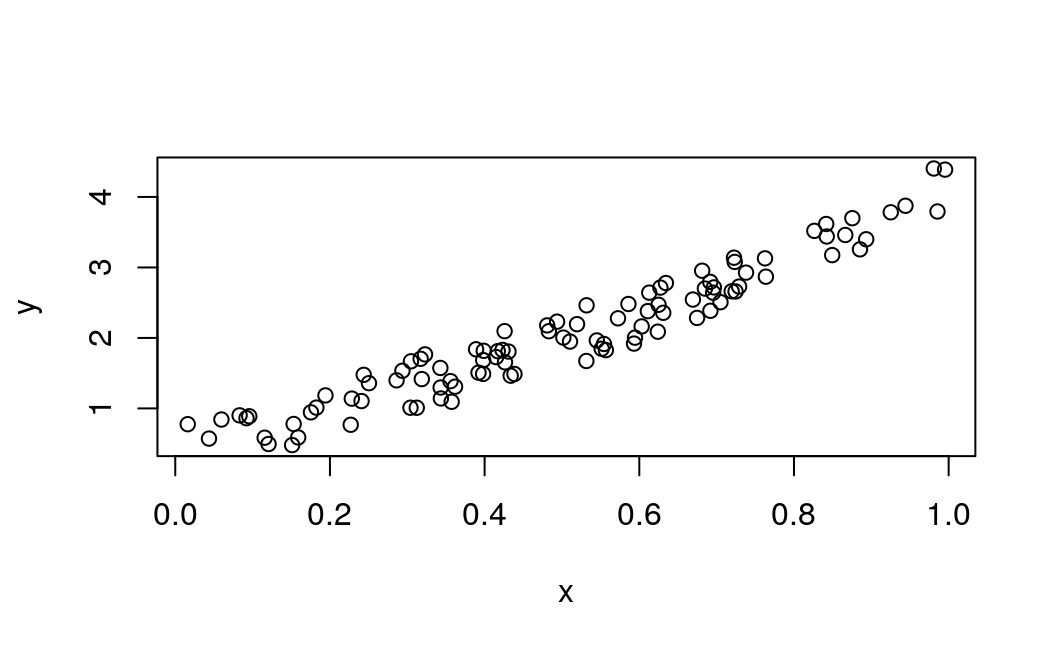
\includegraphics[width=0.7\linewidth]{0406-linear_regression-simple_files/figure-latex/datasets-1} \end{center}

\hypertarget{convert-arrays-to-tensors}{%
\section{Convert arrays to tensors}\label{convert-arrays-to-tensors}}

Before you start the training process, you need to convert the numpy array to Variables that supported by Torch and autograd.

\hypertarget{converting-from-numpy-to-tensor}{%
\section{Converting from numpy to tensor}\label{converting-from-numpy-to-tensor}}

Notice that before converting to a Torch tensor, we need first to convert the R numeric vector to a \texttt{numpy} array:

\begin{Shaded}
\begin{Highlighting}[]
\CommentTok{# convert numpy array to tensor in shape of input size}
\NormalTok{x <-}\StringTok{ }\KeywordTok{r_to_py}\NormalTok{(x)}
\NormalTok{y <-}\StringTok{ }\KeywordTok{r_to_py}\NormalTok{(y)}
\NormalTok{x =}\StringTok{ }\NormalTok{torch}\OperatorTok{$}\KeywordTok{from_numpy}\NormalTok{(x}\OperatorTok{$}\KeywordTok{reshape}\NormalTok{(}\OperatorTok{-}\NormalTok{1L, 1L))}\OperatorTok{$}\KeywordTok{float}\NormalTok{()}
\NormalTok{y =}\StringTok{ }\NormalTok{torch}\OperatorTok{$}\KeywordTok{from_numpy}\NormalTok{(y}\OperatorTok{$}\KeywordTok{reshape}\NormalTok{(}\OperatorTok{-}\NormalTok{1L, 1L))}\OperatorTok{$}\KeywordTok{float}\NormalTok{()}
\KeywordTok{print}\NormalTok{(x, y)}
\CommentTok{#> tensor([[0.6965],}
\CommentTok{#>         [0.2861],}
\CommentTok{#>         [0.2269],}
\CommentTok{#>         [0.5513],}
\CommentTok{#>         [0.7195],}
\CommentTok{#>         [0.4231],}
\CommentTok{#>         [0.9808],}
\CommentTok{#>         [0.6848],}
\CommentTok{#>         [0.4809],}
\CommentTok{#>         [0.3921],}
\CommentTok{#>         [0.3432],}
\CommentTok{#>         [0.7290],}
\CommentTok{#>         [0.4386],}
\CommentTok{#>         [0.0597],}
\CommentTok{#>         [0.3980],}
\CommentTok{#>         [0.7380],}
\CommentTok{#>         [0.1825],}
\CommentTok{#>         [0.1755],}
\CommentTok{#>         [0.5316],}
\CommentTok{#>         [0.5318],}
\CommentTok{#>         [0.6344],}
\CommentTok{#>         [0.8494],}
\CommentTok{#>         [0.7245],}
\CommentTok{#>         [0.6110],}
\CommentTok{#>         [0.7224],}
\CommentTok{#>         [0.3230],}
\CommentTok{#>         [0.3618],}
\CommentTok{#>         [0.2283],}
\CommentTok{#>         [0.2937],}
\CommentTok{#>         [0.6310],}
\CommentTok{#>         [0.0921],}
\CommentTok{#>         [0.4337],}
\CommentTok{#>         [0.4309],}
\CommentTok{#>         [0.4937],}
\CommentTok{#>         [0.4258],}
\CommentTok{#>         [0.3123],}
\CommentTok{#>         [0.4264],}
\CommentTok{#>         [0.8934],}
\CommentTok{#>         [0.9442],}
\CommentTok{#>         [0.5018],}
\CommentTok{#>         [0.6240],}
\CommentTok{#>         [0.1156],}
\CommentTok{#>         [0.3173],}
\CommentTok{#>         [0.4148],}
\CommentTok{#>         [0.8663],}
\CommentTok{#>         [0.2505],}
\CommentTok{#>         [0.4830],}
\CommentTok{#>         [0.9856],}
\CommentTok{#>         [0.5195],}
\CommentTok{#>         [0.6129],}
\CommentTok{#>         [0.1206],}
\CommentTok{#>         [0.8263],}
\CommentTok{#>         [0.6031],}
\CommentTok{#>         [0.5451],}
\CommentTok{#>         [0.3428],}
\CommentTok{#>         [0.3041],}
\CommentTok{#>         [0.4170],}
\CommentTok{#>         [0.6813],}
\CommentTok{#>         [0.8755],}
\CommentTok{#>         [0.5104],}
\CommentTok{#>         [0.6693],}
\CommentTok{#>         [0.5859],}
\CommentTok{#>         [0.6249],}
\CommentTok{#>         [0.6747],}
\CommentTok{#>         [0.8423],}
\CommentTok{#>         [0.0832],}
\CommentTok{#>         [0.7637],}
\CommentTok{#>         [0.2437],}
\CommentTok{#>         [0.1942],}
\CommentTok{#>         [0.5725],}
\CommentTok{#>         [0.0957],}
\CommentTok{#>         [0.8853],}
\CommentTok{#>         [0.6272],}
\CommentTok{#>         [0.7234],}
\CommentTok{#>         [0.0161],}
\CommentTok{#>         [0.5944],}
\CommentTok{#>         [0.5568],}
\CommentTok{#>         [0.1590],}
\CommentTok{#>         [0.1531],}
\CommentTok{#>         [0.6955],}
\CommentTok{#>         [0.3188],}
\CommentTok{#>         [0.6920],}
\CommentTok{#>         [0.5544],}
\CommentTok{#>         [0.3890],}
\CommentTok{#>         [0.9251],}
\CommentTok{#>         [0.8417],}
\CommentTok{#>         [0.3574],}
\CommentTok{#>         [0.0436],}
\CommentTok{#>         [0.3048],}
\CommentTok{#>         [0.3982],}
\CommentTok{#>         [0.7050],}
\CommentTok{#>         [0.9954],}
\CommentTok{#>         [0.3559],}
\CommentTok{#>         [0.7625],}
\CommentTok{#>         [0.5932],}
\CommentTok{#>         [0.6917],}
\CommentTok{#>         [0.1511],}
\CommentTok{#>         [0.3989],}
\CommentTok{#>         [0.2409],}
\CommentTok{#>         [0.3435]])}
\end{Highlighting}
\end{Shaded}

\hypertarget{creating-the-network-model}{%
\section{Creating the network model}\label{creating-the-network-model}}

Our network model is a simple Linear layer with an input and an output shape of one.

And the network output should be like this

\begin{verbatim}
Net(
  (hidden): Linear(in_features=1, out_features=1, bias=True)
)
\end{verbatim}

\begin{Shaded}
\begin{Highlighting}[]
\KeywordTok{py_run_string}\NormalTok{(}\StringTok{"import torch"}\NormalTok{)}
\NormalTok{main =}\StringTok{ }\KeywordTok{py_run_string}\NormalTok{(}
\StringTok{"}
\StringTok{import torch.nn as nn}

\StringTok{class Net(nn.Module):}
\StringTok{   def __init__(self):}
\StringTok{       super(Net, self).__init__()}
\StringTok{       self.layer = torch.nn.Linear(1, 1)}

\StringTok{   def forward(self, x):}
\StringTok{       x = self.layer(x)      }
\StringTok{       return x}
\StringTok{"}\NormalTok{)}


\CommentTok{# build a Linear Rgression model}
\NormalTok{net <-}\StringTok{ }\NormalTok{main}\OperatorTok{$}\KeywordTok{Net}\NormalTok{()}

\KeywordTok{print}\NormalTok{(net)}
\CommentTok{#> Net(}
\CommentTok{#>   (layer): Linear(in_features=1, out_features=1, bias=True)}
\CommentTok{#> )}
\end{Highlighting}
\end{Shaded}

\hypertarget{optimizer-and-loss}{%
\section{Optimizer and Loss}\label{optimizer-and-loss}}

Next, you should define the Optimizer and the Loss Function for our training process.

\begin{Shaded}
\begin{Highlighting}[]
\CommentTok{# Define Optimizer and Loss Function}
\NormalTok{optimizer <-}\StringTok{ }\NormalTok{torch}\OperatorTok{$}\NormalTok{optim}\OperatorTok{$}\KeywordTok{SGD}\NormalTok{(net}\OperatorTok{$}\KeywordTok{parameters}\NormalTok{(), }\DataTypeTok{lr=}\FloatTok{0.2}\NormalTok{)}
\NormalTok{loss_func <-}\StringTok{ }\NormalTok{torch}\OperatorTok{$}\NormalTok{nn}\OperatorTok{$}\KeywordTok{MSELoss}\NormalTok{()}
\KeywordTok{print}\NormalTok{(optimizer)}
\CommentTok{#> SGD (}
\CommentTok{#> Parameter Group 0}
\CommentTok{#>     dampening: 0}
\CommentTok{#>     lr: 0.2}
\CommentTok{#>     momentum: 0}
\CommentTok{#>     nesterov: False}
\CommentTok{#>     weight_decay: 0}
\CommentTok{#> )}
\KeywordTok{print}\NormalTok{(loss_func)}
\CommentTok{#> MSELoss()}
\end{Highlighting}
\end{Shaded}

\hypertarget{training-1}{%
\section{Training}\label{training-1}}

Now let's start our training process. With an epoch of 250, you will iterate our data to find the best value for our hyperparameters.

\begin{Shaded}
\begin{Highlighting}[]
\CommentTok{# x = x$type(torch$float)   # make it a a FloatTensor}
\CommentTok{# y = y$type(torch$float)}

\CommentTok{# x <- torch$as_tensor(x, dtype = torch$float)}
\CommentTok{# y <- torch$as_tensor(y, dtype = torch$float)}

\NormalTok{inputs  =}\StringTok{ }\KeywordTok{Variable}\NormalTok{(x)}
\NormalTok{outputs =}\StringTok{ }\KeywordTok{Variable}\NormalTok{(y)}

\CommentTok{# base plot}
\KeywordTok{plot}\NormalTok{(x}\OperatorTok{$}\NormalTok{data}\OperatorTok{$}\KeywordTok{numpy}\NormalTok{(), y}\OperatorTok{$}\NormalTok{data}\OperatorTok{$}\KeywordTok{numpy}\NormalTok{(), }\DataTypeTok{col =} \StringTok{"blue"}\NormalTok{)}
\ControlFlowTok{for}\NormalTok{ (i }\ControlFlowTok{in} \DecValTok{1}\OperatorTok{:}\DecValTok{250}\NormalTok{) \{}
\NormalTok{   prediction =}\StringTok{ }\KeywordTok{net}\NormalTok{(inputs)}
\NormalTok{   loss =}\StringTok{ }\KeywordTok{loss_func}\NormalTok{(prediction, outputs)}
\NormalTok{   optimizer}\OperatorTok{$}\KeywordTok{zero_grad}\NormalTok{()}
\NormalTok{   loss}\OperatorTok{$}\KeywordTok{backward}\NormalTok{()}
\NormalTok{   optimizer}\OperatorTok{$}\KeywordTok{step}\NormalTok{()}
   
   \ControlFlowTok{if}\NormalTok{ (i }\OperatorTok{>}\StringTok{ }\DecValTok{1}\NormalTok{) }\ControlFlowTok{break}

   \ControlFlowTok{if}\NormalTok{ (i }\OperatorTok\StringTok{ }\DecValTok{10} \OperatorTok{==}\StringTok{ }\DecValTok{0}\NormalTok{) \{}
       \CommentTok{# plot and show learning process}
      \CommentTok{# points(x$data$numpy(), y$data$numpy())}
      \KeywordTok{points}\NormalTok{(x}\OperatorTok{$}\NormalTok{data}\OperatorTok{$}\KeywordTok{numpy}\NormalTok{(), prediction}\OperatorTok{$}\NormalTok{data}\OperatorTok{$}\KeywordTok{numpy}\NormalTok{(), }\DataTypeTok{col=}\StringTok{"red"}\NormalTok{)}
       \CommentTok{# cat(i, loss$data$numpy(), "\textbackslash{}n")}
\NormalTok{   \}}
\NormalTok{\}}
\end{Highlighting}
\end{Shaded}

\begin{center}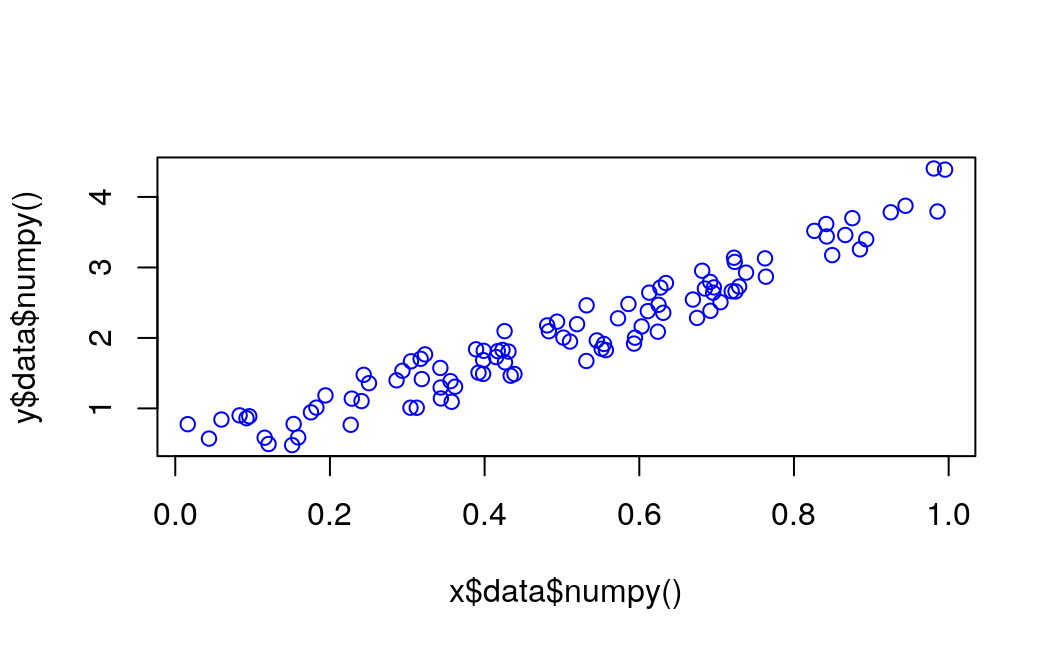
\includegraphics[width=0.7\linewidth]{0406-linear_regression-simple_files/figure-latex/plot-xy-1} \end{center}

\hypertarget{results}{%
\section{Results}\label{results}}

As you can see below, you successfully performed regression with a neural network. Actually, on every iteration, the red line in the plot will update and change its position to fit the data. But in this picture, you only show you the final result.

\hypertarget{rainfall.-linear-regression}{%
\chapter{Rainfall. Linear Regression}\label{rainfall.-linear-regression}}

\begin{Shaded}
\begin{Highlighting}[]
\KeywordTok{library}\NormalTok{(rTorch)}
\end{Highlighting}
\end{Shaded}

Select the device: CPU or GPU

\begin{Shaded}
\begin{Highlighting}[]
\NormalTok{torch}\OperatorTok{$}\KeywordTok{manual_seed}\NormalTok{(}\DecValTok{0}\NormalTok{)}
\CommentTok{#> <torch._C.Generator>}

\NormalTok{device =}\StringTok{ }\NormalTok{torch}\OperatorTok{$}\KeywordTok{device}\NormalTok{(}\StringTok{'cpu'}\NormalTok{)}
\end{Highlighting}
\end{Shaded}

\hypertarget{training-data}{%
\section{Training data}\label{training-data}}

The training data can be represented using 2 matrices (inputs and targets), each with one row per observation, and one column per variable.

\begin{Shaded}
\begin{Highlighting}[]
\CommentTok{# Input (temp, rainfall, humidity)}
\NormalTok{inputs =}\StringTok{ }\NormalTok{np}\OperatorTok{$}\KeywordTok{array}\NormalTok{(}\KeywordTok{list}\NormalTok{(}\KeywordTok{list}\NormalTok{(}\DecValTok{73}\NormalTok{, }\DecValTok{67}\NormalTok{, }\DecValTok{43}\NormalTok{),}
                   \KeywordTok{list}\NormalTok{(}\DecValTok{91}\NormalTok{, }\DecValTok{88}\NormalTok{, }\DecValTok{64}\NormalTok{),}
                   \KeywordTok{list}\NormalTok{(}\DecValTok{87}\NormalTok{, }\DecValTok{134}\NormalTok{, }\DecValTok{58}\NormalTok{),}
                   \KeywordTok{list}\NormalTok{(}\DecValTok{102}\NormalTok{, }\DecValTok{43}\NormalTok{, }\DecValTok{37}\NormalTok{),}
                   \KeywordTok{list}\NormalTok{(}\DecValTok{69}\NormalTok{, }\DecValTok{96}\NormalTok{, }\DecValTok{70}\NormalTok{)), }\DataTypeTok{dtype=}\StringTok{'float32'}\NormalTok{)}

\CommentTok{# Targets (apples, oranges)}
\NormalTok{targets =}\StringTok{ }\NormalTok{np}\OperatorTok{$}\KeywordTok{array}\NormalTok{(}\KeywordTok{list}\NormalTok{(}\KeywordTok{list}\NormalTok{(}\DecValTok{56}\NormalTok{, }\DecValTok{70}\NormalTok{), }
                    \KeywordTok{list}\NormalTok{(}\DecValTok{81}\NormalTok{, }\DecValTok{101}\NormalTok{),}
                    \KeywordTok{list}\NormalTok{(}\DecValTok{119}\NormalTok{, }\DecValTok{133}\NormalTok{),}
                    \KeywordTok{list}\NormalTok{(}\DecValTok{22}\NormalTok{, }\DecValTok{37}\NormalTok{), }
                    \KeywordTok{list}\NormalTok{(}\DecValTok{103}\NormalTok{, }\DecValTok{119}\NormalTok{)), }\DataTypeTok{dtype=}\StringTok{'float32'}\NormalTok{)}
\end{Highlighting}
\end{Shaded}

\hypertarget{convert-arrays-to-tensors-1}{%
\section{Convert arrays to tensors}\label{convert-arrays-to-tensors-1}}

Before we build a model, we need to convert inputs and targets to PyTorch tensors.

\begin{Shaded}
\begin{Highlighting}[]
\CommentTok{# Convert inputs and targets to tensors}
\NormalTok{inputs =}\StringTok{ }\NormalTok{torch}\OperatorTok{$}\KeywordTok{from_numpy}\NormalTok{(inputs)}
\NormalTok{targets =}\StringTok{ }\NormalTok{torch}\OperatorTok{$}\KeywordTok{from_numpy}\NormalTok{(targets)}

\KeywordTok{print}\NormalTok{(inputs)}
\CommentTok{#> tensor([[ 73.,  67.,  43.],}
\CommentTok{#>         [ 91.,  88.,  64.],}
\CommentTok{#>         [ 87., 134.,  58.],}
\CommentTok{#>         [102.,  43.,  37.],}
\CommentTok{#>         [ 69.,  96.,  70.]], dtype=torch.float64)}
\KeywordTok{print}\NormalTok{(targets)}
\CommentTok{#> tensor([[ 56.,  70.],}
\CommentTok{#>         [ 81., 101.],}
\CommentTok{#>         [119., 133.],}
\CommentTok{#>         [ 22.,  37.],}
\CommentTok{#>         [103., 119.]], dtype=torch.float64)}
\end{Highlighting}
\end{Shaded}

The weights and biases can also be represented as matrices, initialized with random values. The first row of \(w\) and the first element of \(b\) are used to predict the first target variable, i.e.~yield for apples, and, similarly, the second for oranges.

\begin{Shaded}
\begin{Highlighting}[]
\CommentTok{# random numbers for weights and biases. Then convert to double()}
\NormalTok{torch}\OperatorTok{$}\KeywordTok{set_default_dtype}\NormalTok{(torch}\OperatorTok{$}\NormalTok{double)}

\NormalTok{w =}\StringTok{ }\NormalTok{torch}\OperatorTok{$}\KeywordTok{randn}\NormalTok{(2L, 3L, }\DataTypeTok{requires_grad=}\OtherTok{TRUE}\NormalTok{)  }\CommentTok{#$double()}
\NormalTok{b =}\StringTok{ }\NormalTok{torch}\OperatorTok{$}\KeywordTok{randn}\NormalTok{(2L, }\DataTypeTok{requires_grad=}\OtherTok{TRUE}\NormalTok{)      }\CommentTok{#$double()}

\KeywordTok{print}\NormalTok{(w)}
\CommentTok{#> tensor([[ 1.5410, -0.2934, -2.1788],}
\CommentTok{#>         [ 0.5684, -1.0845, -1.3986]], requires_grad=True)}
\KeywordTok{print}\NormalTok{(b)}
\CommentTok{#> tensor([0.4033, 0.8380], requires_grad=True)}
\end{Highlighting}
\end{Shaded}

\hypertarget{build-the-model}{%
\section{Build the model}\label{build-the-model}}

The model is simply a function that performs a matrix multiplication of the input \(x\) and the weights \(w\) (transposed), and adds the bias \(b\) (replicated for each observation).

\begin{Shaded}
\begin{Highlighting}[]
\NormalTok{model <-}\StringTok{ }\ControlFlowTok{function}\NormalTok{(x) \{}
\NormalTok{  wt <-}\StringTok{ }\NormalTok{w}\OperatorTok{$}\KeywordTok{t}\NormalTok{()}
  \KeywordTok{return}\NormalTok{(torch}\OperatorTok{$}\KeywordTok{add}\NormalTok{(torch}\OperatorTok{$}\KeywordTok{mm}\NormalTok{(x, wt), b))}
\NormalTok{\}}
\end{Highlighting}
\end{Shaded}

\hypertarget{generate-predictions}{%
\section{Generate predictions}\label{generate-predictions}}

The matrix obtained by passing the input data to the model is a set of predictions for the target variables.

\begin{Shaded}
\begin{Highlighting}[]
\CommentTok{# Generate predictions}
\NormalTok{preds =}\StringTok{ }\KeywordTok{model}\NormalTok{(inputs)}
\KeywordTok{print}\NormalTok{(preds)}
\CommentTok{#> tensor([[  -0.4516,  -90.4691],}
\CommentTok{#>         [ -24.6303, -132.3828],}
\CommentTok{#>         [ -31.2192, -176.1530],}
\CommentTok{#>         [  64.3523,  -39.5645],}
\CommentTok{#>         [ -73.9524, -161.9560]], grad_fn=<AddBackward0>)}
\end{Highlighting}
\end{Shaded}

\begin{Shaded}
\begin{Highlighting}[]
\CommentTok{# Compare with targets}
\KeywordTok{print}\NormalTok{(targets)}
\CommentTok{#> tensor([[ 56.,  70.],}
\CommentTok{#>         [ 81., 101.],}
\CommentTok{#>         [119., 133.],}
\CommentTok{#>         [ 22.,  37.],}
\CommentTok{#>         [103., 119.]])}
\end{Highlighting}
\end{Shaded}

Because we've started with random weights and biases, the model does not a very good job of predicting the target variables.

\hypertarget{loss-function}{%
\section{Loss Function}\label{loss-function}}

We can compare the predictions with the actual targets, using the following method:

\begin{itemize}
\tightlist
\item
  Calculate the difference between the two matrices (preds and targets).
\item
  Square all elements of the difference matrix to remove negative values.
\item
  Calculate the average of the elements in the resulting matrix.
\end{itemize}

The result is a single number, known as the mean squared error (MSE).

\begin{Shaded}
\begin{Highlighting}[]
\CommentTok{# MSE loss}
\NormalTok{mse =}\StringTok{ }\ControlFlowTok{function}\NormalTok{(t1, t2) \{}
\NormalTok{  diff <-}\StringTok{ }\NormalTok{torch}\OperatorTok{$}\KeywordTok{sub}\NormalTok{(t1, t2)}
\NormalTok{  mul <-}\StringTok{ }\NormalTok{torch}\OperatorTok{$}\KeywordTok{sum}\NormalTok{(torch}\OperatorTok{$}\KeywordTok{mul}\NormalTok{(diff, diff))}
  \KeywordTok{return}\NormalTok{(torch}\OperatorTok{$}\KeywordTok{div}\NormalTok{(mul, diff}\OperatorTok{$}\KeywordTok{numel}\NormalTok{()))}
\NormalTok{\}}

\KeywordTok{print}\NormalTok{(mse)}
\CommentTok{#> function(t1, t2) \{}
\CommentTok{#>   diff <- torch$sub(t1, t2)}
\CommentTok{#>   mul <- torch$sum(torch$mul(diff, diff))}
\CommentTok{#>   return(torch$div(mul, diff$numel()))}
\CommentTok{#> \}}
\end{Highlighting}
\end{Shaded}

\hypertarget{step-by-step-process}{%
\section{Step by step process}\label{step-by-step-process}}

\hypertarget{compute-the-losses}{%
\subsection{Compute the losses}\label{compute-the-losses}}

\begin{Shaded}
\begin{Highlighting}[]
\CommentTok{# Compute loss}
\NormalTok{loss =}\StringTok{ }\KeywordTok{mse}\NormalTok{(preds, targets)}
\KeywordTok{print}\NormalTok{(loss)}
\CommentTok{#> tensor(33060.8053, grad_fn=<DivBackward0>)}
\CommentTok{# 46194}
\CommentTok{# 33060.8070}
\end{Highlighting}
\end{Shaded}

The resulting number is called the \textbf{loss}, because it indicates how bad the model is at predicting the target variables. Lower the loss, better the model.

\hypertarget{compute-gradients}{%
\subsection{Compute Gradients}\label{compute-gradients}}

With PyTorch, we can automatically compute the gradient or derivative of the loss w.r.t. to the weights and biases, because they have \texttt{requires\_grad} set to True.

\begin{Shaded}
\begin{Highlighting}[]
\CommentTok{# Compute gradients}
\NormalTok{loss}\OperatorTok{$}\KeywordTok{backward}\NormalTok{()}
\end{Highlighting}
\end{Shaded}

The gradients are stored in the .grad property of the respective tensors.

\begin{Shaded}
\begin{Highlighting}[]
\CommentTok{# Gradients for weights}
\KeywordTok{print}\NormalTok{(w)}
\CommentTok{#> tensor([[ 1.5410, -0.2934, -2.1788],}
\CommentTok{#>         [ 0.5684, -1.0845, -1.3986]], requires_grad=True)}
\KeywordTok{print}\NormalTok{(w}\OperatorTok{$}\NormalTok{grad)}
\CommentTok{#> tensor([[ -6938.4351,  -9674.6757,  -5744.0206],}
\CommentTok{#>         [-17408.7861, -20595.9333, -12453.4702]])}
\end{Highlighting}
\end{Shaded}

\begin{Shaded}
\begin{Highlighting}[]
\CommentTok{# Gradients for bias}
\KeywordTok{print}\NormalTok{(b)}
\CommentTok{#> tensor([0.4033, 0.8380], requires_grad=True)}
\KeywordTok{print}\NormalTok{(b}\OperatorTok{$}\NormalTok{grad)}
\CommentTok{#> tensor([ -89.3802, -212.1051])}
\end{Highlighting}
\end{Shaded}

A key insight from calculus is that the gradient indicates the rate of change of the loss, or the slope of the loss function w.r.t. the weights and biases.

\begin{itemize}
\tightlist
\item
  If a gradient element is positive:

  \begin{itemize}
  \tightlist
  \item
    increasing the element's value slightly will increase the loss.
  \item
    decreasing the element's value slightly will decrease the loss.
  \end{itemize}
\item
  If a gradient element is negative,

  \begin{itemize}
  \tightlist
  \item
    increasing the element's value slightly will decrease the loss.
  \item
    decreasing the element's value slightly will increase the loss.
  \end{itemize}
\end{itemize}

The increase or decrease is proportional to the value of the gradient.

\hypertarget{reset-the-gradients}{%
\subsection{Reset the gradients}\label{reset-the-gradients}}

Finally, we'll reset the gradients to zero before moving forward, because PyTorch accumulates gradients.

\begin{Shaded}
\begin{Highlighting}[]
\CommentTok{# Reset the gradients}
\NormalTok{w}\OperatorTok{$}\NormalTok{grad}\OperatorTok{$}\KeywordTok{zero_}\NormalTok{()}
\CommentTok{#> tensor([[0., 0., 0.],}
\CommentTok{#>         [0., 0., 0.]])}
\NormalTok{b}\OperatorTok{$}\NormalTok{grad}\OperatorTok{$}\KeywordTok{zero_}\NormalTok{()}
\CommentTok{#> tensor([0., 0.])}

\KeywordTok{print}\NormalTok{(w}\OperatorTok{$}\NormalTok{grad)}
\CommentTok{#> tensor([[0., 0., 0.],}
\CommentTok{#>         [0., 0., 0.]])}
\KeywordTok{print}\NormalTok{(b}\OperatorTok{$}\NormalTok{grad)}
\CommentTok{#> tensor([0., 0.])}
\end{Highlighting}
\end{Shaded}

\hypertarget{adjust-weights-and-biases-using-gradient-descent}{%
\subsubsection{Adjust weights and biases using gradient descent}\label{adjust-weights-and-biases-using-gradient-descent}}

We'll reduce the loss and improve our model using the gradient descent algorithm, which has the following steps:

\begin{enumerate}
\def\labelenumi{\arabic{enumi}.}
\tightlist
\item
  Generate predictions
\item
  Calculate the loss
\item
  Compute gradients w.r.t the weights and biases
\item
  Adjust the weights by subtracting a small quantity proportional to the gradient
\item
  Reset the gradients to zero
\end{enumerate}

\begin{Shaded}
\begin{Highlighting}[]
\CommentTok{# Generate predictions}
\NormalTok{preds =}\StringTok{ }\KeywordTok{model}\NormalTok{(inputs)}
\KeywordTok{print}\NormalTok{(preds)}
\CommentTok{#> tensor([[  -0.4516,  -90.4691],}
\CommentTok{#>         [ -24.6303, -132.3828],}
\CommentTok{#>         [ -31.2192, -176.1530],}
\CommentTok{#>         [  64.3523,  -39.5645],}
\CommentTok{#>         [ -73.9524, -161.9560]], grad_fn=<AddBackward0>)}
\end{Highlighting}
\end{Shaded}

\begin{Shaded}
\begin{Highlighting}[]
\CommentTok{# Calculate the loss}
\NormalTok{loss =}\StringTok{ }\KeywordTok{mse}\NormalTok{(preds, targets)}
\KeywordTok{print}\NormalTok{(loss)}
\CommentTok{#> tensor(33060.8053, grad_fn=<DivBackward0>)}
\end{Highlighting}
\end{Shaded}

\begin{Shaded}
\begin{Highlighting}[]
\CommentTok{# Compute gradients}
\NormalTok{loss}\OperatorTok{$}\KeywordTok{backward}\NormalTok{()}

\KeywordTok{print}\NormalTok{(w}\OperatorTok{$}\NormalTok{grad)}
\CommentTok{#> tensor([[ -6938.4351,  -9674.6757,  -5744.0206],}
\CommentTok{#>         [-17408.7861, -20595.9333, -12453.4702]])}
\KeywordTok{print}\NormalTok{(b}\OperatorTok{$}\NormalTok{grad)}
\CommentTok{#> tensor([ -89.3802, -212.1051])}
\end{Highlighting}
\end{Shaded}

\begin{Shaded}
\begin{Highlighting}[]
\CommentTok{# Adjust weights and reset gradients}
\KeywordTok{with}\NormalTok{(torch}\OperatorTok{$}\KeywordTok{no_grad}\NormalTok{(), \{}
  \KeywordTok{print}\NormalTok{(w); }\KeywordTok{print}\NormalTok{(b)    }\CommentTok{# requires_grad attribute remains}
\NormalTok{  w}\OperatorTok{$}\NormalTok{data <-}\StringTok{ }\NormalTok{torch}\OperatorTok{$}\KeywordTok{sub}\NormalTok{(w}\OperatorTok{$}\NormalTok{data, torch}\OperatorTok{$}\KeywordTok{mul}\NormalTok{(w}\OperatorTok{$}\NormalTok{grad}\OperatorTok{$}\NormalTok{data, torch}\OperatorTok{$}\KeywordTok{scalar_tensor}\NormalTok{(}\FloatTok{1e-5}\NormalTok{)))}
\NormalTok{  b}\OperatorTok{$}\NormalTok{data <-}\StringTok{ }\NormalTok{torch}\OperatorTok{$}\KeywordTok{sub}\NormalTok{(b}\OperatorTok{$}\NormalTok{data, torch}\OperatorTok{$}\KeywordTok{mul}\NormalTok{(b}\OperatorTok{$}\NormalTok{grad}\OperatorTok{$}\NormalTok{data, torch}\OperatorTok{$}\KeywordTok{scalar_tensor}\NormalTok{(}\FloatTok{1e-5}\NormalTok{)))}

  \KeywordTok{print}\NormalTok{(w}\OperatorTok{$}\NormalTok{grad}\OperatorTok{$}\NormalTok{data}\OperatorTok{$}\KeywordTok{zero_}\NormalTok{())}
  \KeywordTok{print}\NormalTok{(b}\OperatorTok{$}\NormalTok{grad}\OperatorTok{$}\NormalTok{data}\OperatorTok{$}\KeywordTok{zero_}\NormalTok{())}
\NormalTok{\})}
\CommentTok{#> tensor([[ 1.5410, -0.2934, -2.1788],}
\CommentTok{#>         [ 0.5684, -1.0845, -1.3986]], requires_grad=True)}
\CommentTok{#> tensor([0.4033, 0.8380], requires_grad=True)}
\CommentTok{#> tensor([[0., 0., 0.],}
\CommentTok{#>         [0., 0., 0.]])}
\CommentTok{#> tensor([0., 0.])}

\KeywordTok{print}\NormalTok{(w)}
\CommentTok{#> tensor([[ 1.6104, -0.1967, -2.1213],}
\CommentTok{#>         [ 0.7425, -0.8786, -1.2741]], requires_grad=True)}
\KeywordTok{print}\NormalTok{(b)}
\CommentTok{#> tensor([0.4042, 0.8401], requires_grad=True)}
\end{Highlighting}
\end{Shaded}

With the new weights and biases, the model should have a lower loss.

\begin{Shaded}
\begin{Highlighting}[]
\CommentTok{# Calculate loss}
\NormalTok{preds =}\StringTok{ }\KeywordTok{model}\NormalTok{(inputs)}
\NormalTok{loss =}\StringTok{ }\KeywordTok{mse}\NormalTok{(preds, targets)}
\KeywordTok{print}\NormalTok{(loss)}
\CommentTok{#> tensor(23432.4894, grad_fn=<DivBackward0>)}
\end{Highlighting}
\end{Shaded}

\hypertarget{all-together-train-for-multiple-epochs}{%
\section{All together: train for multiple epochs}\label{all-together-train-for-multiple-epochs}}

To reduce the loss further, we repeat the process of adjusting the weights and biases using the gradients multiple times. Each iteration is called an \textbf{epoch}.

\begin{Shaded}
\begin{Highlighting}[]
\CommentTok{# Running all together}
\CommentTok{# Adjust weights and reset gradients}
\NormalTok{num_epochs <-}\StringTok{ }\DecValTok{100}

\ControlFlowTok{for}\NormalTok{ (i }\ControlFlowTok{in} \DecValTok{1}\OperatorTok{:}\NormalTok{num_epochs) \{}
\NormalTok{  preds =}\StringTok{ }\KeywordTok{model}\NormalTok{(inputs)}
\NormalTok{  loss =}\StringTok{ }\KeywordTok{mse}\NormalTok{(preds, targets)}
\NormalTok{  loss}\OperatorTok{$}\KeywordTok{backward}\NormalTok{()}
  \KeywordTok{with}\NormalTok{(torch}\OperatorTok{$}\KeywordTok{no_grad}\NormalTok{(), \{}
\NormalTok{    w}\OperatorTok{$}\NormalTok{data <-}\StringTok{ }\NormalTok{torch}\OperatorTok{$}\KeywordTok{sub}\NormalTok{(w}\OperatorTok{$}\NormalTok{data, torch}\OperatorTok{$}\KeywordTok{mul}\NormalTok{(w}\OperatorTok{$}\NormalTok{grad, torch}\OperatorTok{$}\KeywordTok{scalar_tensor}\NormalTok{(}\FloatTok{1e-5}\NormalTok{)))}
\NormalTok{    b}\OperatorTok{$}\NormalTok{data <-}\StringTok{ }\NormalTok{torch}\OperatorTok{$}\KeywordTok{sub}\NormalTok{(b}\OperatorTok{$}\NormalTok{data, torch}\OperatorTok{$}\KeywordTok{mul}\NormalTok{(b}\OperatorTok{$}\NormalTok{grad, torch}\OperatorTok{$}\KeywordTok{scalar_tensor}\NormalTok{(}\FloatTok{1e-5}\NormalTok{)))}
    
\NormalTok{    w}\OperatorTok{$}\NormalTok{grad}\OperatorTok{$}\KeywordTok{zero_}\NormalTok{()}
\NormalTok{    b}\OperatorTok{$}\NormalTok{grad}\OperatorTok{$}\KeywordTok{zero_}\NormalTok{()}
\NormalTok{  \})}
\NormalTok{\}}

\CommentTok{# Calculate loss}
\NormalTok{preds =}\StringTok{ }\KeywordTok{model}\NormalTok{(inputs)}
\NormalTok{loss =}\StringTok{ }\KeywordTok{mse}\NormalTok{(preds, targets)}
\KeywordTok{print}\NormalTok{(loss)}
\CommentTok{#> tensor(1258.0216, grad_fn=<DivBackward0>)}

\CommentTok{# predictions}
\NormalTok{preds}
\CommentTok{#> tensor([[ 69.2462,  80.2082],}
\CommentTok{#>         [ 73.7183,  97.2052],}
\CommentTok{#>         [118.5780, 124.9272],}
\CommentTok{#>         [ 89.2282,  92.7052],}
\CommentTok{#>         [ 47.4648,  80.7782]], grad_fn=<AddBackward0>)}

\CommentTok{# Targets}
\NormalTok{targets}
\CommentTok{#> tensor([[ 56.,  70.],}
\CommentTok{#>         [ 81., 101.],}
\CommentTok{#>         [119., 133.],}
\CommentTok{#>         [ 22.,  37.],}
\CommentTok{#>         [103., 119.]])}
\end{Highlighting}
\end{Shaded}

\hypertarget{part-neural-networks}{%
\part{Neural Networks}\label{part-neural-networks}}

\hypertarget{a-very-simple-neural-network}{%
\chapter{A very simple neural network}\label{a-very-simple-neural-network}}

\hypertarget{introduction-1}{%
\section{Introduction}\label{introduction-1}}

Source: \url{https://github.com/jcjohnson/pytorch-examples\#pytorch-nn}

In this example we use the torch \texttt{nn} package to implement our two-layer network:

\hypertarget{select-device}{%
\section{Select device}\label{select-device}}

\begin{Shaded}
\begin{Highlighting}[]
\KeywordTok{library}\NormalTok{(rTorch)}

\NormalTok{device =}\StringTok{ }\NormalTok{torch}\OperatorTok{$}\KeywordTok{device}\NormalTok{(}\StringTok{'cpu'}\NormalTok{)}

\CommentTok{# device = torch.device('cuda') # Uncomment this to run on GPU}
\end{Highlighting}
\end{Shaded}

\begin{itemize}
\tightlist
\item
  \texttt{N} is batch size;
\item
  \texttt{D\_in} is input dimension;
\item
  \texttt{H} is hidden dimension;
\item
  \texttt{D\_out} is output dimension.
\end{itemize}

\hypertarget{create-the-dataset}{%
\section{Create the dataset}\label{create-the-dataset}}

\begin{Shaded}
\begin{Highlighting}[]
\NormalTok{torch}\OperatorTok{$}\KeywordTok{manual_seed}\NormalTok{(}\DecValTok{0}\NormalTok{)}
\CommentTok{#> <torch._C.Generator>}

\NormalTok{N <-}\StringTok{ }\NormalTok{64L; D_in <-}\StringTok{ }\NormalTok{1000L; H <-}\StringTok{ }\NormalTok{100L; D_out <-}\StringTok{ }\NormalTok{10L}

\CommentTok{# Create random Tensors to hold inputs and outputs}
\NormalTok{x =}\StringTok{ }\NormalTok{torch}\OperatorTok{$}\KeywordTok{randn}\NormalTok{(N, D_in, }\DataTypeTok{device=}\NormalTok{device)}
\NormalTok{y =}\StringTok{ }\NormalTok{torch}\OperatorTok{$}\KeywordTok{randn}\NormalTok{(N, D_out, }\DataTypeTok{device=}\NormalTok{device)}
\end{Highlighting}
\end{Shaded}

\hypertarget{define-the-model-1}{%
\section{Define the model}\label{define-the-model-1}}

Use the \texttt{nn} package to define our model as a sequence of layers. \texttt{nn.Sequential} is a Module which contains other Modules, and applies them in sequence to produce its output. Each Linear Module computes output from input using a linear function, and holds internal Tensors for its weight and bias.
After constructing the model we use the \texttt{.to()} method to move it to the
desired device.

\begin{Shaded}
\begin{Highlighting}[]
\NormalTok{model <-}\StringTok{ }\NormalTok{torch}\OperatorTok{$}\NormalTok{nn}\OperatorTok{$}\KeywordTok{Sequential}\NormalTok{(}
\NormalTok{  torch}\OperatorTok{$}\NormalTok{nn}\OperatorTok{$}\KeywordTok{Linear}\NormalTok{(D_in, H),              }\CommentTok{# first layer}
\NormalTok{  torch}\OperatorTok{$}\NormalTok{nn}\OperatorTok{$}\KeywordTok{ReLU}\NormalTok{(),}
\NormalTok{  torch}\OperatorTok{$}\NormalTok{nn}\OperatorTok{$}\KeywordTok{Linear}\NormalTok{(H, D_out))}\OperatorTok{$}\KeywordTok{to}\NormalTok{(device)  }\CommentTok{# output layer}

\KeywordTok{print}\NormalTok{(model)}
\CommentTok{#> Sequential(}
\CommentTok{#>   (0): Linear(in_features=1000, out_features=100, bias=True)}
\CommentTok{#>   (1): ReLU()}
\CommentTok{#>   (2): Linear(in_features=100, out_features=10, bias=True)}
\CommentTok{#> )}
\end{Highlighting}
\end{Shaded}

\hypertarget{loss-function-1}{%
\section{Loss function}\label{loss-function-1}}

The \texttt{nn} package also contains definitions of popular loss functions; in this case we will use Mean Squared Error (\textbf{MSE}) as our loss function. Setting \texttt{reduction=\textquotesingle{}sum\textquotesingle{}} means that we are computing the \emph{sum} of squared errors rather than the mean; this is for consistency with the examples above where we manually compute the loss, but in practice it is more common to use mean squared error as a loss by setting \texttt{reduction=\textquotesingle{}elementwise\_mean\textquotesingle{}}.

\begin{Shaded}
\begin{Highlighting}[]
\NormalTok{loss_fn =}\StringTok{ }\NormalTok{torch}\OperatorTok{$}\NormalTok{nn}\OperatorTok{$}\KeywordTok{MSELoss}\NormalTok{(}\DataTypeTok{reduction =} \StringTok{'sum'}\NormalTok{)}
\end{Highlighting}
\end{Shaded}

\hypertarget{iterate-through-batches}{%
\section{Iterate through batches}\label{iterate-through-batches}}

\begin{Shaded}
\begin{Highlighting}[]
\NormalTok{learning_rate =}\StringTok{ }\FloatTok{1e-4}

\ControlFlowTok{for}\NormalTok{ (t }\ControlFlowTok{in} \DecValTok{1}\OperatorTok{:}\DecValTok{500}\NormalTok{) \{}
  \CommentTok{# Forward pass: compute predicted y by passing x to the model. Module objects}
  \CommentTok{# override the __call__ operator so you can call them like functions. When}
  \CommentTok{# doing so you pass a Tensor of input data to the Module and it produces}
  \CommentTok{# a Tensor of output data.}
\NormalTok{  y_pred =}\StringTok{ }\KeywordTok{model}\NormalTok{(x)}

  \CommentTok{# Compute and print loss. We pass Tensors containing the predicted and true}
  \CommentTok{# values of y, and the loss function returns a Tensor containing the loss.}
\NormalTok{  loss =}\StringTok{ }\KeywordTok{loss_fn}\NormalTok{(y_pred, y)}
  
  \KeywordTok{cat}\NormalTok{(t, }\StringTok{"}\CharTok{\textbackslash{}t}\StringTok{"}\NormalTok{)}
  \KeywordTok{cat}\NormalTok{(loss}\OperatorTok{$}\KeywordTok{item}\NormalTok{(), }\StringTok{"}\CharTok{\textbackslash{}n}\StringTok{"}\NormalTok{)}
  
  \CommentTok{# Zero the gradients before running the backward pass.}
\NormalTok{  model}\OperatorTok{$}\KeywordTok{zero_grad}\NormalTok{()}

  \CommentTok{# Backward pass: compute gradient of the loss with respect to all the learnable}
  \CommentTok{# parameters of the model. Internally, the parameters of each Module are stored}
  \CommentTok{# in Tensors with requires_grad=True, so this call will compute gradients for}
  \CommentTok{# all learnable parameters in the model.}
\NormalTok{  loss}\OperatorTok{$}\KeywordTok{backward}\NormalTok{()}

  \CommentTok{# Update the weights using gradient descent. Each parameter is a Tensor, so}
  \CommentTok{# we can access its data and gradients like we did before.}
  \KeywordTok{with}\NormalTok{(torch}\OperatorTok{$}\KeywordTok{no_grad}\NormalTok{(), \{}
      \ControlFlowTok{for}\NormalTok{ (param }\ControlFlowTok{in} \KeywordTok{iterate}\NormalTok{(model}\OperatorTok{$}\KeywordTok{parameters}\NormalTok{())) \{}
        \CommentTok{# in Python this code is much simpler. In R we have to do some conversions}
        
        \CommentTok{# param$data <- torch$sub(param$data,}
        \CommentTok{#                         torch$mul(param$grad$float(),}
        \CommentTok{#                           torch$scalar_tensor(learning_rate)))}
        
\NormalTok{        param}\OperatorTok{$}\NormalTok{data <-}\StringTok{ }\NormalTok{param}\OperatorTok{$}\NormalTok{data }\OperatorTok{-}\StringTok{ }\NormalTok{param}\OperatorTok{$}\NormalTok{grad }\OperatorTok{*}\StringTok{ }\NormalTok{learning_rate}
\NormalTok{      \}}
\NormalTok{   \})}
\NormalTok{\}  }
\CommentTok{#> 1    628 }
\CommentTok{#> 2    585 }
\CommentTok{#> 3    547 }
\CommentTok{#> 4    513 }
\CommentTok{#> 5    482 }
\CommentTok{#> 6    455 }
\CommentTok{#> 7    430 }
\CommentTok{#> 8    406 }
\CommentTok{#> 9    385 }
\CommentTok{#> 10   364 }
\CommentTok{#> 11   345 }
\CommentTok{#> 12   328 }
\CommentTok{#> 13   311 }
\CommentTok{#> 14   295 }
\CommentTok{#> 15   280 }
\CommentTok{#> 16   265 }
\CommentTok{#> 17   252 }
\CommentTok{#> 18   239 }
\CommentTok{#> 19   226 }
\CommentTok{#> 20   214 }
\CommentTok{#> 21   203 }
\CommentTok{#> 22   192 }
\CommentTok{#> 23   181 }
\CommentTok{#> 24   172 }
\CommentTok{#> 25   162 }
\CommentTok{#> 26   153 }
\CommentTok{#> 27   145 }
\CommentTok{#> 28   137 }
\CommentTok{#> 29   129 }
\CommentTok{#> 30   122 }
\CommentTok{#> 31   115 }
\CommentTok{#> 32   109 }
\CommentTok{#> 33   103 }
\CommentTok{#> 34   96.9 }
\CommentTok{#> 35   91.5 }
\CommentTok{#> 36   86.3 }
\CommentTok{#> 37   81.5 }
\CommentTok{#> 38   76.9 }
\CommentTok{#> 39   72.6 }
\CommentTok{#> 40   68.5 }
\CommentTok{#> 41   64.6 }
\CommentTok{#> 42   61 }
\CommentTok{#> 43   57.6 }
\CommentTok{#> 44   54.3 }
\CommentTok{#> 45   51.3 }
\CommentTok{#> 46   48.5 }
\CommentTok{#> 47   45.8 }
\CommentTok{#> 48   43.2 }
\CommentTok{#> 49   40.9 }
\CommentTok{#> 50   38.6 }
\CommentTok{#> 51   36.5 }
\CommentTok{#> 52   34.5 }
\CommentTok{#> 53   32.7 }
\CommentTok{#> 54   30.9 }
\CommentTok{#> 55   29.3 }
\CommentTok{#> 56   27.8 }
\CommentTok{#> 57   26.3 }
\CommentTok{#> 58   24.9 }
\CommentTok{#> 59   23.7 }
\CommentTok{#> 60   22.4 }
\CommentTok{#> 61   21.3 }
\CommentTok{#> 62   20.2 }
\CommentTok{#> 63   19.2 }
\CommentTok{#> 64   18.2 }
\CommentTok{#> 65   17.3 }
\CommentTok{#> 66   16.5 }
\CommentTok{#> 67   15.7 }
\CommentTok{#> 68   14.9 }
\CommentTok{#> 69   14.2 }
\CommentTok{#> 70   13.5 }
\CommentTok{#> 71   12.9 }
\CommentTok{#> 72   12.3 }
\CommentTok{#> 73   11.7 }
\CommentTok{#> 74   11.1 }
\CommentTok{#> 75   10.6 }
\CommentTok{#> 76   10.1 }
\CommentTok{#> 77   9.67 }
\CommentTok{#> 78   9.24 }
\CommentTok{#> 79   8.82 }
\CommentTok{#> 80   8.42 }
\CommentTok{#> 81   8.05 }
\CommentTok{#> 82   7.69 }
\CommentTok{#> 83   7.35 }
\CommentTok{#> 84   7.03 }
\CommentTok{#> 85   6.72 }
\CommentTok{#> 86   6.43 }
\CommentTok{#> 87   6.16 }
\CommentTok{#> 88   5.9 }
\CommentTok{#> 89   5.65 }
\CommentTok{#> 90   5.41 }
\CommentTok{#> 91   5.18 }
\CommentTok{#> 92   4.97 }
\CommentTok{#> 93   4.76 }
\CommentTok{#> 94   4.57 }
\CommentTok{#> 95   4.38 }
\CommentTok{#> 96   4.2 }
\CommentTok{#> 97   4.03 }
\CommentTok{#> 98   3.87 }
\CommentTok{#> 99   3.72 }
\CommentTok{#> 100  3.57 }
\CommentTok{#> 101  3.43 }
\CommentTok{#> 102  3.29 }
\CommentTok{#> 103  3.17 }
\CommentTok{#> 104  3.04 }
\CommentTok{#> 105  2.92 }
\CommentTok{#> 106  2.81 }
\CommentTok{#> 107  2.7 }
\CommentTok{#> 108  2.6 }
\CommentTok{#> 109  2.5 }
\CommentTok{#> 110  2.41 }
\CommentTok{#> 111  2.31 }
\CommentTok{#> 112  2.23 }
\CommentTok{#> 113  2.14 }
\CommentTok{#> 114  2.06 }
\CommentTok{#> 115  1.99 }
\CommentTok{#> 116  1.91 }
\CommentTok{#> 117  1.84 }
\CommentTok{#> 118  1.77 }
\CommentTok{#> 119  1.71 }
\CommentTok{#> 120  1.65 }
\CommentTok{#> 121  1.59 }
\CommentTok{#> 122  1.53 }
\CommentTok{#> 123  1.47 }
\CommentTok{#> 124  1.42 }
\CommentTok{#> 125  1.37 }
\CommentTok{#> 126  1.32 }
\CommentTok{#> 127  1.27 }
\CommentTok{#> 128  1.23 }
\CommentTok{#> 129  1.18 }
\CommentTok{#> 130  1.14 }
\CommentTok{#> 131  1.1 }
\CommentTok{#> 132  1.06 }
\CommentTok{#> 133  1.02 }
\CommentTok{#> 134  0.989 }
\CommentTok{#> 135  0.954 }
\CommentTok{#> 136  0.921 }
\CommentTok{#> 137  0.889 }
\CommentTok{#> 138  0.858 }
\CommentTok{#> 139  0.828 }
\CommentTok{#> 140  0.799 }
\CommentTok{#> 141  0.772 }
\CommentTok{#> 142  0.745 }
\CommentTok{#> 143  0.719 }
\CommentTok{#> 144  0.695 }
\CommentTok{#> 145  0.671 }
\CommentTok{#> 146  0.648 }
\CommentTok{#> 147  0.626 }
\CommentTok{#> 148  0.605 }
\CommentTok{#> 149  0.584 }
\CommentTok{#> 150  0.564 }
\CommentTok{#> 151  0.545 }
\CommentTok{#> 152  0.527 }
\CommentTok{#> 153  0.509 }
\CommentTok{#> 154  0.492 }
\CommentTok{#> 155  0.476 }
\CommentTok{#> 156  0.46 }
\CommentTok{#> 157  0.444 }
\CommentTok{#> 158  0.43 }
\CommentTok{#> 159  0.415 }
\CommentTok{#> 160  0.402 }
\CommentTok{#> 161  0.388 }
\CommentTok{#> 162  0.375 }
\CommentTok{#> 163  0.363 }
\CommentTok{#> 164  0.351 }
\CommentTok{#> 165  0.339 }
\CommentTok{#> 166  0.328 }
\CommentTok{#> 167  0.318 }
\CommentTok{#> 168  0.307 }
\CommentTok{#> 169  0.297 }
\CommentTok{#> 170  0.287 }
\CommentTok{#> 171  0.278 }
\CommentTok{#> 172  0.269 }
\CommentTok{#> 173  0.26 }
\CommentTok{#> 174  0.252 }
\CommentTok{#> 175  0.244 }
\CommentTok{#> 176  0.236 }
\CommentTok{#> 177  0.228 }
\CommentTok{#> 178  0.221 }
\CommentTok{#> 179  0.214 }
\CommentTok{#> 180  0.207 }
\CommentTok{#> 181  0.2 }
\CommentTok{#> 182  0.194 }
\CommentTok{#> 183  0.187 }
\CommentTok{#> 184  0.181 }
\CommentTok{#> 185  0.176 }
\CommentTok{#> 186  0.17 }
\CommentTok{#> 187  0.165 }
\CommentTok{#> 188  0.159 }
\CommentTok{#> 189  0.154 }
\CommentTok{#> 190  0.149 }
\CommentTok{#> 191  0.145 }
\CommentTok{#> 192  0.14 }
\CommentTok{#> 193  0.136 }
\CommentTok{#> 194  0.131 }
\CommentTok{#> 195  0.127 }
\CommentTok{#> 196  0.123 }
\CommentTok{#> 197  0.119 }
\CommentTok{#> 198  0.115 }
\CommentTok{#> 199  0.112 }
\CommentTok{#> 200  0.108 }
\CommentTok{#> 201  0.105 }
\CommentTok{#> 202  0.102 }
\CommentTok{#> 203  0.0983 }
\CommentTok{#> 204  0.0952 }
\CommentTok{#> 205  0.0923 }
\CommentTok{#> 206  0.0894 }
\CommentTok{#> 207  0.0866 }
\CommentTok{#> 208  0.0838 }
\CommentTok{#> 209  0.0812 }
\CommentTok{#> 210  0.0787 }
\CommentTok{#> 211  0.0762 }
\CommentTok{#> 212  0.0739 }
\CommentTok{#> 213  0.0716 }
\CommentTok{#> 214  0.0693 }
\CommentTok{#> 215  0.0672 }
\CommentTok{#> 216  0.0651 }
\CommentTok{#> 217  0.0631 }
\CommentTok{#> 218  0.0611 }
\CommentTok{#> 219  0.0592 }
\CommentTok{#> 220  0.0574 }
\CommentTok{#> 221  0.0556 }
\CommentTok{#> 222  0.0539 }
\CommentTok{#> 223  0.0522 }
\CommentTok{#> 224  0.0506 }
\CommentTok{#> 225  0.0491 }
\CommentTok{#> 226  0.0476 }
\CommentTok{#> 227  0.0461 }
\CommentTok{#> 228  0.0447 }
\CommentTok{#> 229  0.0433 }
\CommentTok{#> 230  0.042 }
\CommentTok{#> 231  0.0407 }
\CommentTok{#> 232  0.0394 }
\CommentTok{#> 233  0.0382 }
\CommentTok{#> 234  0.0371 }
\CommentTok{#> 235  0.0359 }
\CommentTok{#> 236  0.0348 }
\CommentTok{#> 237  0.0338 }
\CommentTok{#> 238  0.0327 }
\CommentTok{#> 239  0.0317 }
\CommentTok{#> 240  0.0308 }
\CommentTok{#> 241  0.0298 }
\CommentTok{#> 242  0.0289 }
\CommentTok{#> 243  0.028 }
\CommentTok{#> 244  0.0272 }
\CommentTok{#> 245  0.0263 }
\CommentTok{#> 246  0.0255 }
\CommentTok{#> 247  0.0248 }
\CommentTok{#> 248  0.024 }
\CommentTok{#> 249  0.0233 }
\CommentTok{#> 250  0.0226 }
\CommentTok{#> 251  0.0219 }
\CommentTok{#> 252  0.0212 }
\CommentTok{#> 253  0.0206 }
\CommentTok{#> 254  0.02 }
\CommentTok{#> 255  0.0194 }
\CommentTok{#> 256  0.0188 }
\CommentTok{#> 257  0.0182 }
\CommentTok{#> 258  0.0177 }
\CommentTok{#> 259  0.0171 }
\CommentTok{#> 260  0.0166 }
\CommentTok{#> 261  0.0161 }
\CommentTok{#> 262  0.0156 }
\CommentTok{#> 263  0.0151 }
\CommentTok{#> 264  0.0147 }
\CommentTok{#> 265  0.0142 }
\CommentTok{#> 266  0.0138 }
\CommentTok{#> 267  0.0134 }
\CommentTok{#> 268  0.013 }
\CommentTok{#> 269  0.0126 }
\CommentTok{#> 270  0.0122 }
\CommentTok{#> 271  0.0119 }
\CommentTok{#> 272  0.0115 }
\CommentTok{#> 273  0.0112 }
\CommentTok{#> 274  0.0108 }
\CommentTok{#> 275  0.0105 }
\CommentTok{#> 276  0.0102 }
\CommentTok{#> 277  0.00988 }
\CommentTok{#> 278  0.00959 }
\CommentTok{#> 279  0.0093 }
\CommentTok{#> 280  0.00902 }
\CommentTok{#> 281  0.00875 }
\CommentTok{#> 282  0.00849 }
\CommentTok{#> 283  0.00824 }
\CommentTok{#> 284  0.00799 }
\CommentTok{#> 285  0.00775 }
\CommentTok{#> 286  0.00752 }
\CommentTok{#> 287  0.0073 }
\CommentTok{#> 288  0.00708 }
\CommentTok{#> 289  0.00687 }
\CommentTok{#> 290  0.00666 }
\CommentTok{#> 291  0.00647 }
\CommentTok{#> 292  0.00627 }
\CommentTok{#> 293  0.00609 }
\CommentTok{#> 294  0.00591 }
\CommentTok{#> 295  0.00573 }
\CommentTok{#> 296  0.00556 }
\CommentTok{#> 297  0.0054 }
\CommentTok{#> 298  0.00524 }
\CommentTok{#> 299  0.00508 }
\CommentTok{#> 300  0.00493 }
\CommentTok{#> 301  0.00478 }
\CommentTok{#> 302  0.00464 }
\CommentTok{#> 303  0.0045 }
\CommentTok{#> 304  0.00437 }
\CommentTok{#> 305  0.00424 }
\CommentTok{#> 306  0.00412 }
\CommentTok{#> 307  0.00399 }
\CommentTok{#> 308  0.00388 }
\CommentTok{#> 309  0.00376 }
\CommentTok{#> 310  0.00365 }
\CommentTok{#> 311  0.00354 }
\CommentTok{#> 312  0.00344 }
\CommentTok{#> 313  0.00334 }
\CommentTok{#> 314  0.00324 }
\CommentTok{#> 315  0.00314 }
\CommentTok{#> 316  0.00305 }
\CommentTok{#> 317  0.00296 }
\CommentTok{#> 318  0.00287 }
\CommentTok{#> 319  0.00279 }
\CommentTok{#> 320  0.00271 }
\CommentTok{#> 321  0.00263 }
\CommentTok{#> 322  0.00255 }
\CommentTok{#> 323  0.00248 }
\CommentTok{#> 324  0.0024 }
\CommentTok{#> 325  0.00233 }
\CommentTok{#> 326  0.00226 }
\CommentTok{#> 327  0.0022 }
\CommentTok{#> 328  0.00213 }
\CommentTok{#> 329  0.00207 }
\CommentTok{#> 330  0.00201 }
\CommentTok{#> 331  0.00195 }
\CommentTok{#> 332  0.00189 }
\CommentTok{#> 333  0.00184 }
\CommentTok{#> 334  0.00178 }
\CommentTok{#> 335  0.00173 }
\CommentTok{#> 336  0.00168 }
\CommentTok{#> 337  0.00163 }
\CommentTok{#> 338  0.00158 }
\CommentTok{#> 339  0.00154 }
\CommentTok{#> 340  0.00149 }
\CommentTok{#> 341  0.00145 }
\CommentTok{#> 342  0.00141 }
\CommentTok{#> 343  0.00137 }
\CommentTok{#> 344  0.00133 }
\CommentTok{#> 345  0.00129 }
\CommentTok{#> 346  0.00125 }
\CommentTok{#> 347  0.00121 }
\CommentTok{#> 348  0.00118 }
\CommentTok{#> 349  0.00114 }
\CommentTok{#> 350  0.00111 }
\CommentTok{#> 351  0.00108 }
\CommentTok{#> 352  0.00105 }
\CommentTok{#> 353  0.00102 }
\CommentTok{#> 354  0.000987 }
\CommentTok{#> 355  0.000958 }
\CommentTok{#> 356  0.000931 }
\CommentTok{#> 357  0.000904 }
\CommentTok{#> 358  0.000877 }
\CommentTok{#> 359  0.000852 }
\CommentTok{#> 360  0.000827 }
\CommentTok{#> 361  0.000803 }
\CommentTok{#> 362  0.00078 }
\CommentTok{#> 363  0.000757 }
\CommentTok{#> 364  0.000735 }
\CommentTok{#> 365  0.000714 }
\CommentTok{#> 366  0.000693 }
\CommentTok{#> 367  0.000673 }
\CommentTok{#> 368  0.000654 }
\CommentTok{#> 369  0.000635 }
\CommentTok{#> 370  0.000617 }
\CommentTok{#> 371  0.000599 }
\CommentTok{#> 372  0.000581 }
\CommentTok{#> 373  0.000565 }
\CommentTok{#> 374  0.000548 }
\CommentTok{#> 375  0.000532 }
\CommentTok{#> 376  0.000517 }
\CommentTok{#> 377  0.000502 }
\CommentTok{#> 378  0.000488 }
\CommentTok{#> 379  0.000474 }
\CommentTok{#> 380  0.00046 }
\CommentTok{#> 381  0.000447 }
\CommentTok{#> 382  0.000434 }
\CommentTok{#> 383  0.000421 }
\CommentTok{#> 384  0.000409 }
\CommentTok{#> 385  0.000397 }
\CommentTok{#> 386  0.000386 }
\CommentTok{#> 387  0.000375 }
\CommentTok{#> 388  0.000364 }
\CommentTok{#> 389  0.000354 }
\CommentTok{#> 390  0.000343 }
\CommentTok{#> 391  0.000334 }
\CommentTok{#> 392  0.000324 }
\CommentTok{#> 393  0.000315 }
\CommentTok{#> 394  0.000306 }
\CommentTok{#> 395  0.000297 }
\CommentTok{#> 396  0.000288 }
\CommentTok{#> 397  0.00028 }
\CommentTok{#> 398  0.000272 }
\CommentTok{#> 399  0.000264 }
\CommentTok{#> 400  0.000257 }
\CommentTok{#> 401  0.000249 }
\CommentTok{#> 402  0.000242 }
\CommentTok{#> 403  0.000235 }
\CommentTok{#> 404  0.000228 }
\CommentTok{#> 405  0.000222 }
\CommentTok{#> 406  0.000216 }
\CommentTok{#> 407  0.000209 }
\CommentTok{#> 408  0.000203 }
\CommentTok{#> 409  0.000198 }
\CommentTok{#> 410  0.000192 }
\CommentTok{#> 411  0.000186 }
\CommentTok{#> 412  0.000181 }
\CommentTok{#> 413  0.000176 }
\CommentTok{#> 414  0.000171 }
\CommentTok{#> 415  0.000166 }
\CommentTok{#> 416  0.000161 }
\CommentTok{#> 417  0.000157 }
\CommentTok{#> 418  0.000152 }
\CommentTok{#> 419  0.000148 }
\CommentTok{#> 420  0.000144 }
\CommentTok{#> 421  0.00014 }
\CommentTok{#> 422  0.000136 }
\CommentTok{#> 423  0.000132 }
\CommentTok{#> 424  0.000128 }
\CommentTok{#> 425  0.000124 }
\CommentTok{#> 426  0.000121 }
\CommentTok{#> 427  0.000117 }
\CommentTok{#> 428  0.000114 }
\CommentTok{#> 429  0.000111 }
\CommentTok{#> 430  0.000108 }
\CommentTok{#> 431  0.000105 }
\CommentTok{#> 432  0.000102 }
\CommentTok{#> 433  9.87e-05 }
\CommentTok{#> 434  9.59e-05 }
\CommentTok{#> 435  9.32e-05 }
\CommentTok{#> 436  9.06e-05 }
\CommentTok{#> 437  8.8e-05 }
\CommentTok{#> 438  8.55e-05 }
\CommentTok{#> 439  8.31e-05 }
\CommentTok{#> 440  8.07e-05 }
\CommentTok{#> 441  7.84e-05 }
\CommentTok{#> 442  7.62e-05 }
\CommentTok{#> 443  7.41e-05 }
\CommentTok{#> 444  7.2e-05 }
\CommentTok{#> 445  6.99e-05 }
\CommentTok{#> 446  6.79e-05 }
\CommentTok{#> 447  6.6e-05 }
\CommentTok{#> 448  6.41e-05 }
\CommentTok{#> 449  6.23e-05 }
\CommentTok{#> 450  6.06e-05 }
\CommentTok{#> 451  5.89e-05 }
\CommentTok{#> 452  5.72e-05 }
\CommentTok{#> 453  5.56e-05 }
\CommentTok{#> 454  5.4e-05 }
\CommentTok{#> 455  5.25e-05 }
\CommentTok{#> 456  5.1e-05 }
\CommentTok{#> 457  4.96e-05 }
\CommentTok{#> 458  4.82e-05 }
\CommentTok{#> 459  4.68e-05 }
\CommentTok{#> 460  4.55e-05 }
\CommentTok{#> 461  4.42e-05 }
\CommentTok{#> 462  4.3e-05 }
\CommentTok{#> 463  4.18e-05 }
\CommentTok{#> 464  4.06e-05 }
\CommentTok{#> 465  3.94e-05 }
\CommentTok{#> 466  3.83e-05 }
\CommentTok{#> 467  3.72e-05 }
\CommentTok{#> 468  3.62e-05 }
\CommentTok{#> 469  3.52e-05 }
\CommentTok{#> 470  3.42e-05 }
\CommentTok{#> 471  3.32e-05 }
\CommentTok{#> 472  3.23e-05 }
\CommentTok{#> 473  3.14e-05 }
\CommentTok{#> 474  3.05e-05 }
\CommentTok{#> 475  2.96e-05 }
\CommentTok{#> 476  2.88e-05 }
\CommentTok{#> 477  2.8e-05 }
\CommentTok{#> 478  2.72e-05 }
\CommentTok{#> 479  2.65e-05 }
\CommentTok{#> 480  2.57e-05 }
\CommentTok{#> 481  2.5e-05 }
\CommentTok{#> 482  2.43e-05 }
\CommentTok{#> 483  2.36e-05 }
\CommentTok{#> 484  2.29e-05 }
\CommentTok{#> 485  2.23e-05 }
\CommentTok{#> 486  2.17e-05 }
\CommentTok{#> 487  2.11e-05 }
\CommentTok{#> 488  2.05e-05 }
\CommentTok{#> 489  1.99e-05 }
\CommentTok{#> 490  1.94e-05 }
\CommentTok{#> 491  1.88e-05 }
\CommentTok{#> 492  1.83e-05 }
\CommentTok{#> 493  1.78e-05 }
\CommentTok{#> 494  1.73e-05 }
\CommentTok{#> 495  1.68e-05 }
\CommentTok{#> 496  1.63e-05 }
\CommentTok{#> 497  1.59e-05 }
\CommentTok{#> 498  1.54e-05 }
\CommentTok{#> 499  1.5e-05 }
\CommentTok{#> 500  1.46e-05}
\end{Highlighting}
\end{Shaded}

These two expression are equivalent, with the first being the long version natural way of doing it in \textbf{PyTorch}. The second is using the generics in R for subtraction, multiplication and scalar conversion.

\begin{verbatim}
param$data <- torch$sub(param$data,
                        torch$mul(param$grad$float(),
                          torch$scalar_tensor(learning_rate)))
}
\end{verbatim}

\begin{verbatim}
param$data <- param$data - param$grad * learning_rate
\end{verbatim}

\hypertarget{neural-networks-2}{%
\chapter{Neural Networks 2}\label{neural-networks-2}}

Source: \url{https://github.com/jcjohnson/pytorch-examples\#pytorch-nn}

\hypertarget{nn2-1}{%
\section{nn2 1}\label{nn2-1}}

\hypertarget{nn2-2}{%
\section{nn2 2}\label{nn2-2}}

\hypertarget{part-image-recognition}{%
\part{Image Recognition}\label{part-image-recognition}}

\hypertarget{part-pytorch-and-r-data-structures}{%
\part{PyTorch and R data structures}\label{part-pytorch-and-r-data-structures}}

\hypertarget{working-with-data.frame}{%
\chapter{Working with data.frame}\label{working-with-data.frame}}

\hypertarget{load-pytorch-libraries}{%
\section{Load PyTorch libraries}\label{load-pytorch-libraries}}

\begin{Shaded}
\begin{Highlighting}[]
\KeywordTok{library}\NormalTok{(rTorch)}

\NormalTok{torch       <-}\StringTok{ }\KeywordTok{import}\NormalTok{(}\StringTok{"torch"}\NormalTok{)}
\NormalTok{torchvision <-}\StringTok{ }\KeywordTok{import}\NormalTok{(}\StringTok{"torchvision"}\NormalTok{)}
\NormalTok{nn          <-}\StringTok{ }\KeywordTok{import}\NormalTok{(}\StringTok{"torch.nn"}\NormalTok{)}
\NormalTok{transforms  <-}\StringTok{ }\KeywordTok{import}\NormalTok{(}\StringTok{"torchvision.transforms"}\NormalTok{)}
\NormalTok{dsets       <-}\StringTok{ }\KeywordTok{import}\NormalTok{(}\StringTok{"torchvision.datasets"}\NormalTok{)}
\NormalTok{builtins    <-}\StringTok{ }\KeywordTok{import_builtins}\NormalTok{()}
\NormalTok{np          <-}\StringTok{ }\KeywordTok{import}\NormalTok{(}\StringTok{"numpy"}\NormalTok{)}
\end{Highlighting}
\end{Shaded}

\hypertarget{dataset-iteration-batch-settings}{%
\section{Dataset iteration batch settings}\label{dataset-iteration-batch-settings}}

\begin{Shaded}
\begin{Highlighting}[]
\CommentTok{# folders where the images are located}
\NormalTok{train_data_path =}\StringTok{ '~/mnist_png_full/training/'}
\NormalTok{test_data_path  =}\StringTok{ '~/mnist_png_full/testing/'}
\end{Highlighting}
\end{Shaded}

\begin{Shaded}
\begin{Highlighting}[]
\CommentTok{# read the datasets without normalization}
\NormalTok{train_dataset =}\StringTok{ }\NormalTok{torchvision}\OperatorTok{$}\NormalTok{datasets}\OperatorTok{$}\KeywordTok{ImageFolder}\NormalTok{(}\DataTypeTok{root =}\NormalTok{ train_data_path, }
    \DataTypeTok{transform =}\NormalTok{ torchvision}\OperatorTok{$}\NormalTok{transforms}\OperatorTok{$}\KeywordTok{ToTensor}\NormalTok{()}
\NormalTok{)}

\KeywordTok{print}\NormalTok{(train_dataset)}
\CommentTok{#> Dataset ImageFolder}
\CommentTok{#>     Number of datapoints: 60000}
\CommentTok{#>     Root location: /home/msfz751/mnist_png_full/training/}
\end{Highlighting}
\end{Shaded}

\hypertarget{summary-statistics-for-tensors}{%
\section{Summary statistics for tensors}\label{summary-statistics-for-tensors}}

\hypertarget{using-data.frame}{%
\section{\texorpdfstring{using \texttt{data.frame}}{using data.frame}}\label{using-data.frame}}

\begin{Shaded}
\begin{Highlighting}[]
\KeywordTok{library}\NormalTok{(tictoc)}
\KeywordTok{tic}\NormalTok{()}

\NormalTok{fun_list <-}\StringTok{ }\KeywordTok{list}\NormalTok{(}
    \DataTypeTok{size  =} \KeywordTok{c}\NormalTok{(}\StringTok{"size"}\NormalTok{),}
    \DataTypeTok{numel =} \KeywordTok{c}\NormalTok{(}\StringTok{"numel"}\NormalTok{),}
    \DataTypeTok{sum   =} \KeywordTok{c}\NormalTok{(}\StringTok{"sum"}\NormalTok{,    }\StringTok{"item"}\NormalTok{),}
    \DataTypeTok{mean  =} \KeywordTok{c}\NormalTok{(}\StringTok{"mean"}\NormalTok{,   }\StringTok{"item"}\NormalTok{),}
    \DataTypeTok{std   =} \KeywordTok{c}\NormalTok{(}\StringTok{"std"}\NormalTok{,    }\StringTok{"item"}\NormalTok{),}
    \DataTypeTok{med   =} \KeywordTok{c}\NormalTok{(}\StringTok{"median"}\NormalTok{, }\StringTok{"item"}\NormalTok{),}
    \DataTypeTok{max   =} \KeywordTok{c}\NormalTok{(}\StringTok{"max"}\NormalTok{,    }\StringTok{"item"}\NormalTok{),}
    \DataTypeTok{min   =} \KeywordTok{c}\NormalTok{(}\StringTok{"min"}\NormalTok{,    }\StringTok{"item"}\NormalTok{)}
\NormalTok{    )}

\NormalTok{idx <-}\StringTok{ }\KeywordTok{seq}\NormalTok{(0L, 599L)    }\CommentTok{# how many samples}

\NormalTok{fun_get_tensor <-}\StringTok{ }\ControlFlowTok{function}\NormalTok{(x) }\KeywordTok{py_get_item}\NormalTok{(train_dataset, x)[[}\DecValTok{1}\NormalTok{]]}

\NormalTok{stat_fun <-}\StringTok{ }\ControlFlowTok{function}\NormalTok{(x, str_fun) \{}
\NormalTok{  fun_var <-}\StringTok{ }\KeywordTok{paste0}\NormalTok{(}\StringTok{"fun_get_tensor(x)"}\NormalTok{, }\StringTok{"$"}\NormalTok{, str_fun, }\StringTok{"()"}\NormalTok{)}
  \KeywordTok{sapply}\NormalTok{(idx, }\ControlFlowTok{function}\NormalTok{(x) }
    \KeywordTok{ifelse}\NormalTok{(}\KeywordTok{is.numeric}\NormalTok{(}\KeywordTok{eval}\NormalTok{(}\KeywordTok{parse}\NormalTok{(}\DataTypeTok{text =}\NormalTok{ fun_var))),  }\CommentTok{# size return chracater}
           \KeywordTok{eval}\NormalTok{(}\KeywordTok{parse}\NormalTok{(}\DataTypeTok{text =}\NormalTok{ fun_var)),              }\CommentTok{# all else are numeric}
           \KeywordTok{as.character}\NormalTok{(}\KeywordTok{eval}\NormalTok{(}\KeywordTok{parse}\NormalTok{(}\DataTypeTok{text =}\NormalTok{ fun_var)))))}
\NormalTok{\}  }

\NormalTok{df <-}\StringTok{ }\KeywordTok{data.frame}\NormalTok{(}\DataTypeTok{ridx =}\NormalTok{ idx}\OperatorTok{+}\DecValTok{1}\NormalTok{,      }\CommentTok{# index number for the sample}
  \KeywordTok{do.call}\NormalTok{(data.frame, }
          \KeywordTok{lapply}\NormalTok{(}
              \KeywordTok{sapply}\NormalTok{(fun_list, }\ControlFlowTok{function}\NormalTok{(x) }\KeywordTok{paste}\NormalTok{(x, }\DataTypeTok{collapse =} \StringTok{"()$"}\NormalTok{)), }
              \ControlFlowTok{function}\NormalTok{(y) }\KeywordTok{stat_fun}\NormalTok{(}\DecValTok{1}\NormalTok{, y)}
\NormalTok{          )}
\NormalTok{  )}
\NormalTok{)}
\KeywordTok{head}\NormalTok{(df)}
\CommentTok{#>   ridx                    size numel sum  mean   std med max min}
\CommentTok{#> 1    1 torch.Size([3, 28, 28])  2352 366 0.156 0.329   0   1   0}
\CommentTok{#> 2    2 torch.Size([3, 28, 28])  2352 284 0.121 0.297   0   1   0}
\CommentTok{#> 3    3 torch.Size([3, 28, 28])  2352 645 0.274 0.420   0   1   0}
\CommentTok{#> 4    4 torch.Size([3, 28, 28])  2352 410 0.174 0.355   0   1   0}
\CommentTok{#> 5    5 torch.Size([3, 28, 28])  2352 321 0.137 0.312   0   1   0}
\CommentTok{#> 6    6 torch.Size([3, 28, 28])  2352 654 0.278 0.421   0   1   0}
\KeywordTok{toc}\NormalTok{()}
\CommentTok{#> 12.504 sec elapsed}
\CommentTok{# 59    1.663s}
\CommentTok{#   599  13.5s}
\CommentTok{#  5999  54.321 sec; 137.6s}
\CommentTok{# 59999 553.489 sec elapsed}
\end{Highlighting}
\end{Shaded}

\hypertarget{working-with-data.table}{%
\chapter{Working with data.table}\label{working-with-data.table}}

\hypertarget{load-pytorch-libraries-1}{%
\section{Load PyTorch libraries}\label{load-pytorch-libraries-1}}

\begin{Shaded}
\begin{Highlighting}[]
\KeywordTok{library}\NormalTok{(rTorch)}

\NormalTok{torch       <-}\StringTok{ }\KeywordTok{import}\NormalTok{(}\StringTok{"torch"}\NormalTok{)}
\NormalTok{torchvision <-}\StringTok{ }\KeywordTok{import}\NormalTok{(}\StringTok{"torchvision"}\NormalTok{)}
\NormalTok{nn          <-}\StringTok{ }\KeywordTok{import}\NormalTok{(}\StringTok{"torch.nn"}\NormalTok{)}
\NormalTok{transforms  <-}\StringTok{ }\KeywordTok{import}\NormalTok{(}\StringTok{"torchvision.transforms"}\NormalTok{)}
\NormalTok{dsets       <-}\StringTok{ }\KeywordTok{import}\NormalTok{(}\StringTok{"torchvision.datasets"}\NormalTok{)}
\NormalTok{builtins    <-}\StringTok{ }\KeywordTok{import_builtins}\NormalTok{()}
\NormalTok{np          <-}\StringTok{ }\KeywordTok{import}\NormalTok{(}\StringTok{"numpy"}\NormalTok{)}

\CommentTok{## Dataset iteration batch settings}
\CommentTok{# folders where the images are located}
\NormalTok{train_data_path =}\StringTok{ '~/mnist_png_full/training/'}
\NormalTok{test_data_path  =}\StringTok{ '~/mnist_png_full/testing/'}

\CommentTok{# read the datasets without normalization}
\NormalTok{train_dataset =}\StringTok{ }\NormalTok{torchvision}\OperatorTok{$}\NormalTok{datasets}\OperatorTok{$}\KeywordTok{ImageFolder}\NormalTok{(}\DataTypeTok{root =}\NormalTok{ train_data_path, }
    \DataTypeTok{transform =}\NormalTok{ torchvision}\OperatorTok{$}\NormalTok{transforms}\OperatorTok{$}\KeywordTok{ToTensor}\NormalTok{()}
\NormalTok{)}

\KeywordTok{print}\NormalTok{(train_dataset)}
\CommentTok{#> Dataset ImageFolder}
\CommentTok{#>     Number of datapoints: 60000}
\CommentTok{#>     Root location: /home/msfz751/mnist_png_full/training/}
\end{Highlighting}
\end{Shaded}

\hypertarget{using-data.table}{%
\subsection{Using `data.table}\label{using-data.table}}

\begin{Shaded}
\begin{Highlighting}[]
\KeywordTok{library}\NormalTok{(data.table)}
\KeywordTok{library}\NormalTok{(tictoc)}
\KeywordTok{tic}\NormalTok{()}

\NormalTok{fun_list <-}\StringTok{ }\KeywordTok{list}\NormalTok{(}
    \DataTypeTok{numel =} \KeywordTok{c}\NormalTok{(}\StringTok{"numel"}\NormalTok{),}
    \DataTypeTok{sum   =} \KeywordTok{c}\NormalTok{(}\StringTok{"sum"}\NormalTok{,    }\StringTok{"item"}\NormalTok{),}
    \DataTypeTok{mean  =} \KeywordTok{c}\NormalTok{(}\StringTok{"mean"}\NormalTok{,   }\StringTok{"item"}\NormalTok{),}
    \DataTypeTok{std   =} \KeywordTok{c}\NormalTok{(}\StringTok{"std"}\NormalTok{,    }\StringTok{"item"}\NormalTok{),}
    \DataTypeTok{med   =} \KeywordTok{c}\NormalTok{(}\StringTok{"median"}\NormalTok{, }\StringTok{"item"}\NormalTok{),}
    \DataTypeTok{max   =} \KeywordTok{c}\NormalTok{(}\StringTok{"max"}\NormalTok{,    }\StringTok{"item"}\NormalTok{),}
    \DataTypeTok{min   =} \KeywordTok{c}\NormalTok{(}\StringTok{"min"}\NormalTok{,    }\StringTok{"item"}\NormalTok{)}
\NormalTok{    )}

\NormalTok{idx <-}\StringTok{ }\KeywordTok{seq}\NormalTok{(0L, 5999L)}

\NormalTok{fun_get_tensor <-}\StringTok{ }\ControlFlowTok{function}\NormalTok{(x) }\KeywordTok{py_get_item}\NormalTok{(train_dataset, x)[[}\DecValTok{1}\NormalTok{]]}

\NormalTok{stat_fun <-}\StringTok{ }\ControlFlowTok{function}\NormalTok{(x, str_fun) \{}
\NormalTok{  fun_var <-}\StringTok{ }\KeywordTok{paste0}\NormalTok{(}\StringTok{"fun_get_tensor(x)"}\NormalTok{, }\StringTok{"$"}\NormalTok{, str_fun, }\StringTok{"()"}\NormalTok{)}
  \KeywordTok{sapply}\NormalTok{(idx, }\ControlFlowTok{function}\NormalTok{(x) }
    \KeywordTok{ifelse}\NormalTok{(}\KeywordTok{is.numeric}\NormalTok{(}\KeywordTok{eval}\NormalTok{(}\KeywordTok{parse}\NormalTok{(}\DataTypeTok{text =}\NormalTok{ fun_var))),  }\CommentTok{# size return chracater}
           \KeywordTok{eval}\NormalTok{(}\KeywordTok{parse}\NormalTok{(}\DataTypeTok{text =}\NormalTok{ fun_var)),              }\CommentTok{# all else are numeric}
           \KeywordTok{as.character}\NormalTok{(}\KeywordTok{eval}\NormalTok{(}\KeywordTok{parse}\NormalTok{(}\DataTypeTok{text =}\NormalTok{ fun_var)))))}
\NormalTok{\}  }

\NormalTok{dt <-}\StringTok{ }\KeywordTok{data.table}\NormalTok{(}\DataTypeTok{ridx =}\NormalTok{ idx}\OperatorTok{+}\DecValTok{1}\NormalTok{,}
  \KeywordTok{do.call}\NormalTok{(data.table, }
          \KeywordTok{lapply}\NormalTok{(}
            \KeywordTok{sapply}\NormalTok{(fun_list, }\ControlFlowTok{function}\NormalTok{(x) }\KeywordTok{paste}\NormalTok{(x, }\DataTypeTok{collapse =} \StringTok{"()$"}\NormalTok{)), }
            \ControlFlowTok{function}\NormalTok{(y) }\KeywordTok{stat_fun}\NormalTok{(}\DecValTok{1}\NormalTok{, y)}
\NormalTok{          )}
\NormalTok{  )}
\NormalTok{)}

\KeywordTok{head}\NormalTok{(dt)}
\CommentTok{#>    ridx numel sum  mean   std med max min}
\CommentTok{#> 1:    1  2352 366 0.156 0.329   0   1   0}
\CommentTok{#> 2:    2  2352 284 0.121 0.297   0   1   0}
\CommentTok{#> 3:    3  2352 645 0.274 0.420   0   1   0}
\CommentTok{#> 4:    4  2352 410 0.174 0.355   0   1   0}
\CommentTok{#> 5:    5  2352 321 0.137 0.312   0   1   0}
\CommentTok{#> 6:    6  2352 654 0.278 0.421   0   1   0}
\KeywordTok{toc}\NormalTok{()}
\CommentTok{#> 112.584 sec elapsed}

\CommentTok{#   60   1.266 sec elapsed}
\CommentTok{#  600   11.798 sec elapsed; 12.9s}
\CommentTok{# 6000  119.256 sec elapsed; 132.9s}
\CommentTok{# 1117.619 sec elapsed}
\end{Highlighting}
\end{Shaded}

\cleardoublepage

\hypertarget{appendix-appendix}{%
\appendix}


\hypertarget{appendixA}{%
\chapter{Statistical Background}\label{appendixA}}

\hypertarget{basic-statistical-terms}{%
\section{Basic statistical terms}\label{basic-statistical-terms}}

\hypertarget{mean}{%
\subsection{Mean}\label{mean}}

The mean is the most commonly reported measure of center. It is commonly called the ``average'' though this term can be a little ambiguous. The mean is the sum of all of the data elements divided by how many elements there are. If we have \(n\) data points, the mean is given by: \[Mean = \frac{x_1 + x_2 + \cdots + x_n}{n}\]

\hypertarget{median}{%
\subsection{Median}\label{median}}

The median is calculated by first sorting a variable's data from smallest to largest. After sorting the data, the middle element in the list is the \textbf{median}. If the middle falls between two values, then the median is the mean of those two values.

\hypertarget{standard-deviation}{%
\subsection{Standard deviation}\label{standard-deviation}}

We will next discuss the \textbf{standard deviation} of a sample dataset pertaining to one variable. The formula can be a little intimidating at first but it is important to remember that it is essentially a measure of how far to expect a given data value is from its mean:

\[Standard \, deviation = \sqrt{\frac{(x_1 - Mean)^2 + (x_2 - Mean)^2 + \cdots + (x_n - Mean)^2}{n - 1}}\]

\hypertarget{five-number-summary}{%
\subsection{Five-number summary}\label{five-number-summary}}

The \textbf{five-number summary} consists of five values: minimum, first quantile AKA 25\textsuperscript{th} percentile, second quantile AKA median AKA 50\textsuperscript{th} percentile, third quantile AKA 75\textsuperscript{th}, and maximum. The quantiles are calculated as

\begin{itemize}
\tightlist
\item
  first quantile (\(Q_1\)): the median of the first half of the sorted data
\item
  third quantile (\(Q_3\)): the median of the second half of the sorted data
\end{itemize}

The \emph{interquartile range} is defined as \(Q_3 - Q_1\) and is a measure of how spread out the middle 50\% of values is. The five-number summary is not influenced by the presence of outliers in the ways that the mean and standard deviation are. It is, thus, recommended for skewed datasets.

\hypertarget{distribution}{%
\subsection{Distribution}\label{distribution}}

The \textbf{distribution} of a variable/dataset corresponds to generalizing patterns in the dataset. It often shows how frequently elements in the dataset appear. It shows how the data varies and gives some information about where a typical element in the data might fall. Distributions are most easily seen through data visualization.

\hypertarget{outliers}{%
\subsection{Outliers}\label{outliers}}

\textbf{Outliers} correspond to values in the dataset that fall far outside the range of ``ordinary'' values. In regards to a boxplot (by default), they correspond to values below \(Q_1 - (1.5 * IQR)\) or above \(Q_3 + (1.5 * IQR)\).

Note that these terms (aside from \textbf{Distribution}) only apply to quantitative variables.

\bibliography{book.bib,packages.bib}


\end{document}
